\documentclass[10pt]{article}
\usepackage[margin=1in]{geometry}
\usepackage{graphicx}
\graphicspath{{./images/}}

\usepackage{amsmath, amssymb, amsthm, amsfonts, mathtools, bbm, breqn}
\usepackage[shortlabels]{enumitem}       % for shortlabels
\usepackage{multicol}       % multiple columns
\usepackage{abraces}        % asymmetric braces
\usepackage{skull}
\usepackage{tikz}
\usepackage{pgfplots}
\usetikzlibrary{arrows.meta, arrows, calc, matrix, positioning, arrows.meta}

\usepackage{hyperref}
\usepackage[capitalize]{cleveref}


% Citing theorems by name. (source: https://tex.stackexchange.com/questions/109843/cleveref-and-named-theorems)
\makeatletter
\newcommand{\ncref}[1]{\cref{#1}\mynameref{#1}{\csname r@#1\endcsname}}

\def\mynameref#1#2{%
  \begingroup
  \edef\@mytxt{#2}%
  \edef\@mytst{\expandafter\@thirdoffive\@mytxt}%
  \ifx\@mytst\empty\else
  \space(\nameref{#1})\fi
  \endgroup
}
\makeatother

% for the pipe symbol
\usepackage[T1]{fontenc}

\usepackage{xcolor} % Enables a broader range of colors

% Define custom colors
\definecolor{RoyalBlue}{cmyk}{1, 0.50, 0, 0}

% Note commands
\definecolor{Red}{rgb}{1,0,0}
\definecolor{Blue}{rgb}{0,0,1}
\definecolor{Purple}{rgb}{.75,0,.25}
\newcommand{\rnote}[1]{\textcolor{Red}{[#1]}}       % Red note
\newcommand{\pnote}[1]{\textcolor{Purple}{[#1]}}    % Purple note
\newcommand{\bnote}[1]{\textcolor{Blue}{#1}}        % Blue text
\newcommand{\Max}[1]{\pnote{#1}}                    % Alias for purple note

% Emphasized text
\newcommand{\demph}[1]{\textcolor{RoyalBlue}{\textbf{\slshape #1}}} % Slanted RoyalBlue text


% Claim numbering (the counter restarts after each proof environment)
\newcounter{claimcount}
\setcounter{claimcount}{0}
\newenvironment{claim}{\refstepcounter{claimcount}\par\addvspace{\medskipamount}\noindent\textbf{Claim \arabic{claimcount}:}}{}
\usepackage{etoolbox}
\AtBeginEnvironment{proof}{\setcounter{claimcount}{0}}
\newenvironment{claimproof}{\par\addvspace{\medskipamount}\noindent\textit{Proof of Claim  \arabic{claimcount}.}}{\hfill\ensuremath{\qedsymbol} \tiny{Claim}

  \medskip}
% Add claim support to cleverref
\crefname{claimcount}{Claim}{Claims}

\usepackage[most]{tcolorbox} % for boxed text,
                             % use \begin{tcolorbox[width=0.7\linewidth,
                             % colback=white, colframe=black]}

\usepackage{empheq} % for boxed equations
\usepackage[most]{tcolorbox}
\newtcbox{\mymath}[1][]{%
  nobeforeafter, math upper, tcbox raise base,
  enhanced, colframe=blue!30!black,
  colback=blue!30, boxrule=1pt,
  #1}
\newtcbox{\boxmath}[1][]{%
  nobeforeafter, math upper, tcbox raise base,
  enhanced, colframe=blue!30!black,
  boxrule=1pt,
  #1}


\newenvironment{augmentedmatrix}[1] % environment for making augmented matrix
{\left[\begin{array}{#1}}
    {\end{array}\right]}



% Math Environments
\newtheorem{theorem}{Theorem}
\newtheorem{assumption}[theorem]{Assumption}
\newtheorem{lemma}[theorem]{Lemma}
\newtheorem{proposition}[theorem]{Proposition}
\newtheorem{corollary}[theorem]{Corollary}
\newtheorem{question}[theorem]{Question}
\theoremstyle{definition}
\newtheorem{definition}[theorem]{Definition}
\newtheorem{remark}[theorem]{Remark}
\newtheorem{example}[theorem]{Example}
\newtheorem{notation}[theorem]{Notation}
\newtheorem{problem}[theorem]{Problem}

% Redefine the Example environment to include "End of example [number]"
\makeatletter
\let\oldexample\example
\renewenvironment{example}
{\begin{oldexample}}
  {\par\smallskip\hfill   End of Example~\theexample. $\square$    \par\end{oldexample}}
\makeatother

% Custom Math Commands
\newcommand{\vt}{\vspace{5mm}}                       % Vertical space
\newcommand{\fl}[1]{\noindent\textbf{#1}}            % Bold first line
\newcommand{\Fl}[1]{\vspace{5mm}\noindent\textbf{#1}}% Bold first line with space above
\newcommand{\norm}[1]{\left\lVert #1 \right\rVert}   % Norm

% Common math symbols
\newcommand{\R}{\mathbb{R}}           % Real numbers
\newcommand{\N}{\mathbb{N}}           % Natural numbers
\newcommand{\C}{\mathbb{C}}           % Complex numbers
\newcommand{\Z}{\mathbb{Z}}           % Integers
\newcommand{\Q}{\mathbb{Q}}           % Rational numbers
\newcommand{\E}{\mathbb{E}}           % Expectation
\renewcommand{\P}{\mathbb{P}}         % Probability (renamed to avoid \P clash)
\newcommand{\indep}{\perp\!\!\!\perp} % Independence symbol

% Operators
\newcommand{\Var}{\mathrm{Var}}   % Variance
\newcommand{\tr}{\mathrm{tr}}     % Trace
\newcommand{\dist}{\mathrm{dist}} % Distance
\newcommand{\diag}{\mathrm{diag}} % diag
\newcommand{\Span}{\mathrm{Span}} % span
\newcommand{\range}{\mathrm{range}} % range
\newcommand{\rank}{\mathrm{rank}} % rank


\usepackage{biblatex}
\addbibresource{refs.bib}

\title{Lecture Notes for Math 307:\\Linear Algebra and Differential Equations}
\author{Instructor: Max Hill (Fall 2025)}
\date{Last updated: \today}
\begin{document}

\maketitle
\tableofcontents

\section*{About this document}

These lecture notes were prepared by Max Hill for a 16-week linear algebra course  (MATH
307) at University of Hawaii at Manoa in Fall 2025.

The textbook used is \textit{Linear Algebra and Differential Equations} (2002)
by G.~Peterson S.~Sochacki, in which we cover primarily Chapters 1,2,5, and 6


\newpage
\setcounter{section}{-1}
\section{Tentative Course Outline}

\begin{itemize}
  \item \textbf{Weeks 1-3: Matrices and determinants.} \textit{(Systems of linear
  equations, matrices, matrix operations, inverse matrices, special matrices
  and their properties, and determinants.)}
  \begin{itemize} 
    \item Section 1.1: Systems of Linear Equations
    \item Section 1.2: Matrices and Matrix Operations
    \item Section 1.3: Inverses of Matrices
    \item Section 1.4: Special Matrices and Additional Properties of Matrices
    \item Section 1.5: Determinants
    \item Section 1.6: Further Properties of Determinants
    \item Section 1.7: Proofs of Theorems on Determinants
  \end{itemize}

  \item \textbf{Weeks 4-6: Vector spaces.} \textit{(Vector spaces, subspaces, spanning
  sets, linear independence, bases, dimension, null space, row and column
  spaces, Wronskian.)}
  \begin{itemize}
    \item Section 2.1: Vector Spaces
    \item Section 2.2: Subspaces and Spanning Sets
    \item Section 2.3: Linear Independence and Bases
    \item Section 2.4: Dimension; Nullspace, Rowspace, and Column Space
    \item Section 2.5: Wronskians
  \end{itemize}
  \item \textbf{Weeks 7-11: Linear transformations, spectral theory.} \textit{(Linear
  transformation, eigenvalues and eigenvectors, algebra of linear
  transformations, matrices for linear transformations, eigenvalues and
  eigenvectors, similar matrices, diagonalization, Jordan normal form.)}
  \begin{itemize}
    \item Section 5.1: Linear Transformations
    \item Section 5.2: The Algebra of Linear Transformations
    \item Section 5.3: Matrices for Linear Transformations
    \item Section 5.4: Eigenvalues and Eigenvectors of Matrices
    \item Section 5.5: Similar Matrices, Diagonalization, and Jordan Canonical Form
    \item Section 5.6: Eigenvectors and Eigenvalues of Linear Transformations
  \end{itemize}
  \item \textbf{Midterm Exam}
  \item \textbf{Weeks 12-14: Systems of differential equations.} \textit{(Theory of
  systems of linear differential equations, homogeneous systems with constant
  coefficients, the diagonalizable case, nondiagonalizable case,
  nonhomogeneous linear systems, applications to $2\times 2$ and $3\times 3$
  systems of nonlinear differential equations.)}
  \begin{itemize}
    \item Section 6.1: The Theory of Systems of Linear Differential Equations
    \item Section 6.2: Homogenous Systems with Constant Coefficients: The
    Diagonalizable Case
    \item Section 6.3: Homogenous Systems with Constant Coefficients: The
    Nondiagonalizable Case
    \item Section 6.4: Nonhomogeneous Linear Systems
    \item Section 6.6: Applications Involving Systems of Linear Differential Equations
    \item Section 6.7: $2\times 2$ Systems of Nonlinear Differential Equations
  \end{itemize}
  \item \textbf{Weeks 14-16: Other stuff if time allows.} \textit{(Converting differential
  equations to first order systems (section 6.5), linearization of $2 \times 2$ nonlinear
  systems (???), stability and instability (section 6.7), predator-prey
  equations (section 6.7.1).)}
  \item \textbf{Final Exam}
\end{itemize}

\newpage
\section{2025-08-25 | Week 01 | Lecture 01}
\textit{This lecture is based on textbook section 1.1. Introduction to Systems
  of Linear Equations}

\begin{center}
  \begin{tcolorbox}[width=0.9\textwidth, colback=white, colframe=black]
    \textit{\textbf{The nexus question of this lecture:} What is a system of
      linear equations, and what does it mean to `solve' a system of linear
      equations?}
  \end{tcolorbox}
\end{center}

\subsection{A first example of a system of linear equations}
We begin with something concrete.


\begin{example}[A first example of a \textit{system of linear equations}]
  \label{ex:a-first-example-linear-system-equations}
  Consider the following word problem:

  \begin{quote}
    \textit{A boat travels between two ports on a river 48 miles apart. When traveling
      downstream (i.e., with the current), the trip takes 4 hours, but when
      traveling upstream (i.e., fighting the current), the trip takes 6 hours.}

    \textit{Assume that the boat and the current are both moving at a
      constant speed. What is the speed of the boat in still water, and what is
      the speed of the current?}
  \end{quote}
  This problem is hard to reason through without writing something down, but
  becomes much simpler when we formalize it mathematically with equations. The
  unknowns are (1) \textbf{the speed of the boat in still water} and (2)
  \textbf{the speed of the current}. So let
  \begin{align*}
    x &:= \text{(the speed of the boat in still water)}\\
    y &:= \text{(the speed of the current)}.
  \end{align*}
  The speed of the boat going downstream is $x+y$. Therefore, since
  $(\text{speed})\times (\text{time})= (\text{distance travelled})$, we have
  \begin{equation*}
    4(x+y)=48, \quad \text{or equivalently} \quad  x+y = 12.
  \end{equation*}
  Similarly, the sped of the boat going upstream is $x-y$, so
  \begin{equation*}
    6(x-y)=48, \quad \text{or equivalently} \quad  x-y = 8
  \end{equation*}
  Thus, we have the following \textit{system of linear equations:}
  \begin{equation}\label{eq:first-example-equations}
    \left\{ \begin{array}{l@{}l} x+y=12 \\x-y=8.  \end{array}\right.
  \end{equation}
  This system has \textbf{two equations} and \textbf{two variables} ($x$ and
  $y$).  You have encountered systems of equations like this many times.
  With the help of the technology of algebra, solving this problem (namely,
  solving System \eqref{eq:first-example-equations}) is much easier than solving the
  original word problem.

 
  \begin{itemize}
    \item In this case, the problem can be easily solved
    \textbf{algebraically} using a substitution (e.g., plug $x=8+y$ into the
    first equation and solve for $y$, then solve for $x$ after finding $y$).
    This gives the solution $(x,y) = (10,2)$. The speed of the boat in still
    water is 10mph. The speed of the river current is 2mph.
    \item We can conceive of another type of solution, which uses a
    \textbf{geometric}, rather than algebraic perspective: observe that each
    equation $x+y=12$ and $x-y=8$ represents a line on the $xy$-plane. Plot
    the lines. Their intersection is the point $(10,2)$, which is the
    solution.
    \item However, solving systems of equations like in
    \eqref{eq:first-example-equations} becomes more cumbersome when there are
    lots of variables and equations. Doing substitutions and algebraic
    manipulations will still work, but will be tedius and difficult if you
    have many equations and variables.

    Later, we will introduce a general algorithm which can solve any such
    system. This algorithm is called \demph{Gauss-Jordan elimination}, and it
    will be one of the core techniques that we will use to solve many types of
    problems in this class.
  \end{itemize}
\end{example}


\subsection{Key definitions: linear systems and their solutions}
In this section, we formalize the mathematical objects we are studying.

\begin{definition}[Linear equation]
  \label{def:linear-equation}
  A \demph{linear equation} in the variables $x_{1},\ldots,x_{n}$ is an
  equation that can be written in the form
  \begin{equation*}
    a_{1}x_{1}+a_{2}x_{2}+\ldots+a_{n}x_{n} = b,
  \end{equation*}
  where $a_{1},\ldots,a_{n}$ and $b$ are constants (e.g., fixed real numbers).
  The numbers $a_{1},\ldots,a_{n}$ are called \demph{coefficients}. 
\end{definition}

Note that the variables $x_{1},\ldots,x_{n}$ are not raised to any powers.
That's what makes the equation \textit{linear}. If we had squares or cubes of
some of the $x_{i}$'s, or products like $x_{1}x_{3}$, then the equation would
be quadratic or cubic, or something else, but not linear.

\begin{example}[Examples of linear equations]
  \label{ex:examples-linear-equations-first-examples}
  \begin{itemize}
    \item[]
    \item The equation
    \begin{equation*}
      2x-3y =1
    \end{equation*}
    is a linear equation in the variables $x$ and $y$. Its graph is a line on the
    $xy$-plane.
    \item The equation
    \begin{equation*}
      3x-y+2z = 9
    \end{equation*}
    is a linear equation in the variables $x,y$ and $z$. Its graph is a plane
    in 3-dimensional space (denoted $\R^{3}$).
    \item The equation
    \begin{equation*}
      -x_{1} +5 x_{2}+ \pi^{2} x_{3}+ \sqrt{2}x_{4} = e^{2}
    \end{equation*}
    is a linear equation in the variables $x_{1},x_{2},x_{3},$ and $x_{4}$.
    The coefficients are
    \begin{equation*}
      a_{1} = -1, \quad a_{2} = 5, \quad a_{3} = \pi, \quad \text{and} \quad a_{4}=\sqrt{2}.
    \end{equation*}
    The graph of this linear system is a 3-dimensional hyperplane in 4d-space
    (i.e., $\R^{4}$).

    \fl{Observation:} In these examples, we observe a simple relationship
    between the number of variables and the dimension of the graph:
    \begin{equation*}
      \text{(dimension of graph)} = (\text{\# of variables}) - 1.
    \end{equation*}
    Here, the term \demph{dimension} refers to the number of free variables.
    In the first equation (which is $2x-3y=1$), it's easy to see that if we
    know one of the variables, then the other one is automatically determined.
    So it makes sense that the graph of this equation is of dimension 1 (which
    it is, because it's a line). For the second equation, if we know any $2$
    of the variables, then the third variable is automatically determined, so
    it makes sense that the dimension of the graph is $2$ (which it is,
    because planes are 2-dimensional). Etc.
  \end{itemize}

\end{example}
\begin{definition}[Linear system, solution of a linear system]
  When considered together, a collection of $m$ linear equations
  \begin{equation}\label{eq:defn-system-of-linear-equations}
    \left\{ \begin{array}{l@{}l}
        \ a_{11}x_{1}+a_{12}x_{2}+\ldots+a_{1n}x_{n} = b_{1} \\
        \ a_{21}x_{1}+a_{21}x_{2}+\ldots+a_{2n}x_{n} = b_{2} \\
        \hfill\vdots\hfill \\
        a_{m1}x_{1}+a_{m2}x_{2}+\ldots+a_{mn}x_{n} = b_{m}
      \end{array}\right.
  \end{equation}
  is called a \demph{system of linear equations}, or \demph{linear system} for
  short. A \demph{solution} to a system of linear equations is a set of values
  for $x_{1},\ldots,x_{n}$ which satisfy all equations in
  system \eqref{eq:defn-system-of-linear-equations}.
\end{definition}

\begin{example}[A system of linear equations]
  \label{ex:system-linear-equations-first-example}
  An example of a system of linear equations is
  \begin{equation*}
    \left\{ \begin{array}{l@{}l}
        \hphantom{-2}x\; -\;  \hphantom{3}y \;+\;  \hphantom{4}z =\hphantom{-}0 \\
        \hphantom{-}2x\;-\; 3y\;+\; 4z= -2 \\
        -2x\;-\; \hphantom{3}y\;+\; \hphantom{4}z=\hphantom{-}7
      \end{array}\right.
  \end{equation*}
  When a linear system like this walks in the door, we always first ask two
  basic questions: (1) `how many equations does it have?' and (2) `how many
  variables does it have?'. In this case, we have $m=3$ equations and $n=3$
  variables.
\end{example}
\subsection{How to understand solutions of linear systems geometrically}
Here is a very useful geometric perspective. In
system \eqref{eq:defn-system-of-linear-equations}, we have a system of $m$ equations
expressed in $n$ variables $x_{1},\ldots,x_{n}$. Each of the $m$ equations is
the equation of some hyperplane\footnote{Note: Hyperplanes will be defined
  more formally later, but for now can be thought of as generalized lines or
  planes, since a 1-dimensional hyperplanes is a \textit{line} and a
  2-dimensional hyperplane is a \textit{plane}.} which lives in
$n$-dimensional space ($\R^{n}$). \textit{The solution to the linear system is the
  intersection of these hyperplanes.}

For example, in \cref{ex:system-linear-equations-first-example}, the
`hyperplanes' were lines, and their intersection was the point $(x,y)=(10,2)$.


We will spend a lot of time understanding what hyperplanes look like, and what
intersections of hyperplanes look like.



\newpage
\section{2025-08-27 | Week 01 | Lecture 02}

\begin{center}
  \begin{tcolorbox}[width=0.9\textwidth, colback=white, colframe=black]
    \textit{\textbf{The nexus question of this lecture:} What do solutions to
      linear systems look like?}
      % \vspace{.5em}
      % \begin{enumerate}
      %   \item How do we understand solutions of linear systems geometrically?
      %   \item How can we find a solution to a linear system algebraically,
      %   without resorting to substitution?
      % \end{enumerate}}
  \end{tcolorbox}
\end{center}
\subsection{How to understand solutions of linear systems geometrically}
Here is a very useful geometric perspective. In
system \eqref{eq:defn-system-of-linear-equations}, we have a system of $m$ equations
expressed in $n$ variables $x_{1},\ldots,x_{n}$. Each of the $m$ equations is
the equation of some hyperplane\footnote{Note: Hyperplanes will be defined
  more formally later, but for now can be thought of as generalized lines or
  planes, since a 1-dimensional hyperplanes is a \textit{line} and a
  2-dimensional hyperplane is a \textit{plane}.} which lives in
$n$-dimensional space ($\R^{n}$). \textit{The solution to the linear system is the
intersection of these hyperplanes.}

The clearest example of this can be seen in the linear system:

\begin{example}[The case with two variables]
  \label{ex:case-with-two-variables}
  \begin{equation}\label{eq:2x2-geometric-intuition-example}
    \left\{ \begin{array}{l@{}l}
        a_{11}x + a_{12}y = b_{1}\\
        a_{21}x + a_{22}y = b_{2}\\
      \end{array}\right.
  \end{equation}
  where $a_{12},a_{22}\neq 0$. (In this case, the ``hyperplanes'' are simply
  lines.) Here, the solutions to the first equation are the points on the line
  \begin{equation}\label{eq:line-1}
    y = -\frac{a_{11}}{a_{12}}x + \frac{b_{1}}{a_{12}}
  \end{equation}
  Similarly, the solutions to the second equation are the points on the line
  \begin{equation}\label{eq:line-2}
    y = - \frac{a_{21}}{a_{22}}x + \frac{b_{2}}{a_{22}}.
  \end{equation}
  There are three possible things that can happen when we intersect the two
  lines in \cref{eq:line-1,eq:line-2}:
  \begin{itemize}
    \item \textbf{Case 1.} The two line equations \cref{eq:line-1,eq:line-2}
    represent distinct lines and are not parallel. In this case, their
    intersection consists of a unique point, like this:
    \begin{center}
      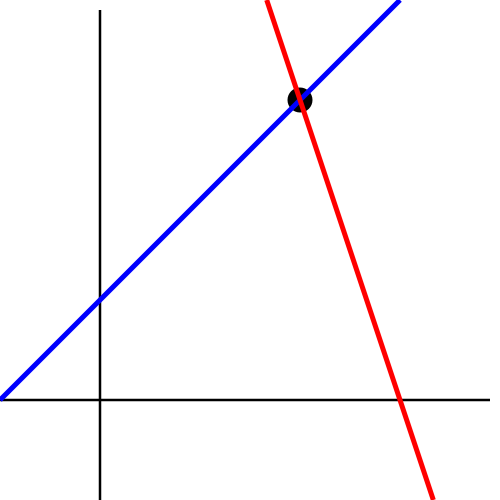
\includegraphics[scale=.12]{images/intersecting-lines} % wikipeida
    \end{center}
    In this case, the system \eqref{eq:2x2-geometric-intuition-example} has
    \textbf{exactly one solution}---namely, the intersection of the two lines,
    just like we saw in the boat example.
  
    \item \textbf{Case 2.} The two line equations \cref{eq:line-1,eq:line-2}
    represent two parallel but different lines. In this case, the two lines
    never intersect each other (i.e., there is no point that lies on both
    lines), so the system \eqref{eq:2x2-geometric-intuition-example} has
    \textbf{no solutions}.
  
    \item \textbf{Case 3.} The two equations of lines are the same, so they
    represent the same line. Therefore the intersection of the two lines is
    the entire line. Therefore, there are \textbf{infinitely many solutions}
    to the linear system \eqref{eq:2x2-geometric-intuition-example}. Namely,
    any point $(x,y)$ on the line is a solution to the linear system.
  \end{itemize}
\end{example}
These three cases desribed in \cref{ex:case-with-two-variables} constitute the
following trichotomy:

\begin{theorem}
  A system of linear equations either has (1) exactly one
  solution, (2) no solution, or (3) infinitely many solutions.
\end{theorem}

We haven't proven this fact, only illustrated it for systems of linear
equations like \eqref{eq:2x2-geometric-intuition-example} that have 2
equations and 2 variables. In fact, as we shall see, this fact always holds
for all linear systems of the form given in
\eqref{eq:defn-system-of-linear-equations}, no matter how many equations and
variables.

\subsection{The planar case}
Recall that, geometrically, a line is determined by two features:
\begin{enumerate}
  \item A slope $m$ which determines the direction of the line
  \item A point $(x_{0},y_{0})$ which the line passes through, as this
  determines where the line lives on the $xy$-plane
\end{enumerate}
It is easy to see that these two things determine everything about a line
because the equation of a line can be expressed as
\begin{equation*}
  y-y_{0} = m(x-x_{0})
\end{equation*}
and to write this down, all we need are $m$ and $(x_{0},y_{0}).$

Just like a line, a plane is determined by two things:
\begin{enumerate}
  \item A normal vector $n= \left\langle A,B,C \right\rangle$ which
  determines the tilt of the plane. (Here, $A,B,$ and $C$ are fixed constants)
  \item A point $(x_{0},y_{0},z_{0})$ which the plane passes through, as this
  determines where in 3-d space $(\R^{3})$ the plane lives.
\end{enumerate}
To be precise, a plane $\P$ consists of the set of points $(x,y,z)$ satisfying
the following equation:
\begin{equation}\label{eq:definition-normal-form-eq-of-plane}
  A(x-x_{0}) + B(y-y_{0})+C(z-z_{0})=0
\end{equation}
This is the standard form equation of a plane, and we can write it down if we
know both $n=\left\langle A,B,C \right\rangle $ and $(x_{0},y_{0},z_{0})$. So
if we know those two things, then we know the equation of the plane, meaning
we know everything about it.

By a little bit of algebra, we can rewrite
\cref{eq:definition-normal-form-eq-of-plane} as
\begin{equation*}
  Ax+By+Cz=D
\end{equation*}
where $D = Ax_{0}+By_{0}+Cz_{0}$. This is a linear equation. Just like how the
solutions to a linear equation with 2 variables form a line, the solutions to
a linear equation with 3 variables form a plane.
\begin{example}[A system with three variables]
  \label{ex:system-with-three-variables}
  Suppose we wish to solve the linear system
  \begin{equation*}
    \left\{
      \begin{alignedat}{4}
        &x &{}\;-\; y &{}\;+\; &z{}&= &0 & \\
        2&x&{}\;-\; 3y&{}+\; 4&z{}&= -&2 & \\
        -2&x&{}\;-\; y&{}\;+\; &z {}&= &7& 
      \end{alignedat}
    \right.
  \end{equation*}
  In this case, each equation is the equation of a plane. The planes for the
  first two equations are the following:
  \begin{center}
    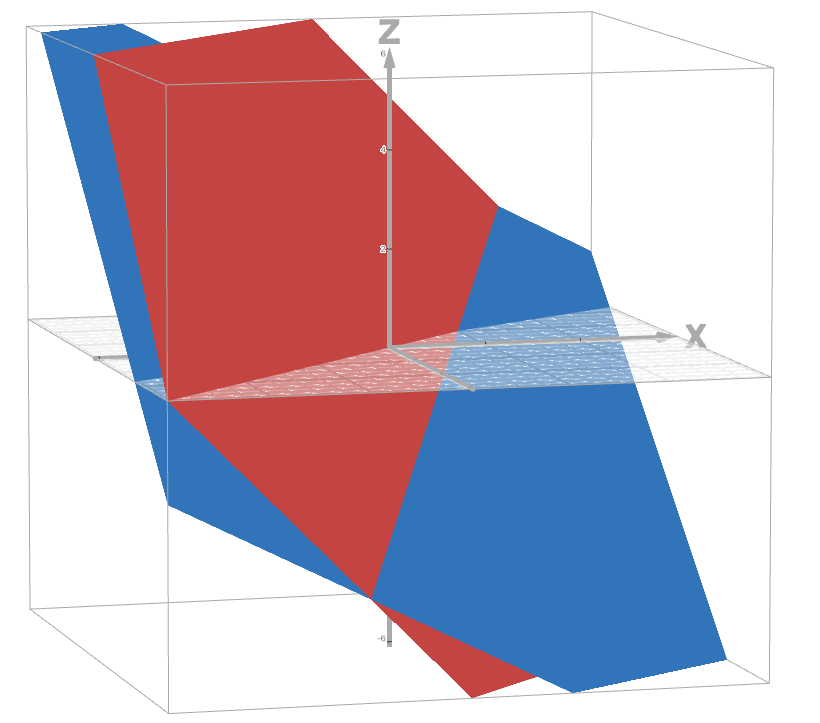
\includegraphics[scale=.2]{images/two-planes}
  \end{center}
  The plane for the first equation is in red. The plane for the second
  equation is blue. Any point on the red plane is a solution to the first
  equation $x-y+z=0$. Any point on the blue plane is a solution to the second
  equation $2x-3y+4z=-2$. The two planes interesect in a line. If I pick any
  point on this line, then it satisfies both equations.

  But our system has three equations, so we have a third plane, and the
  intersection of all three planes is a point, as shown:
  \begin{center}
    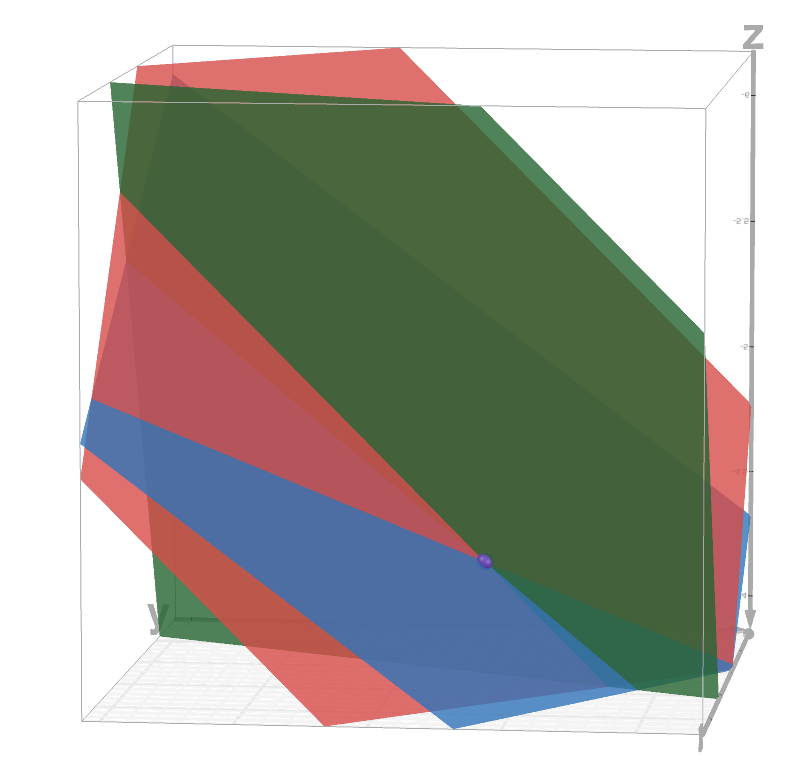
\includegraphics[scale=.2]{images/three-planes-intersection}
  \end{center}
  In this case, the system of equations has a unique solution, which is the
  unique point of intersection of the planes. Here's the desmos link to see
  the plots of these three planes, if you want to play around with them:
  \begin{center}
    \url{https://www.desmos.com/3d/gpgtw2rjaf}
  \end{center}

  Of course there are other ways that three planes could have intersected. For
  example, two of the planes might be parallel, like the following picture, in
  which case the system will have no solutions:
  \begin{center}
    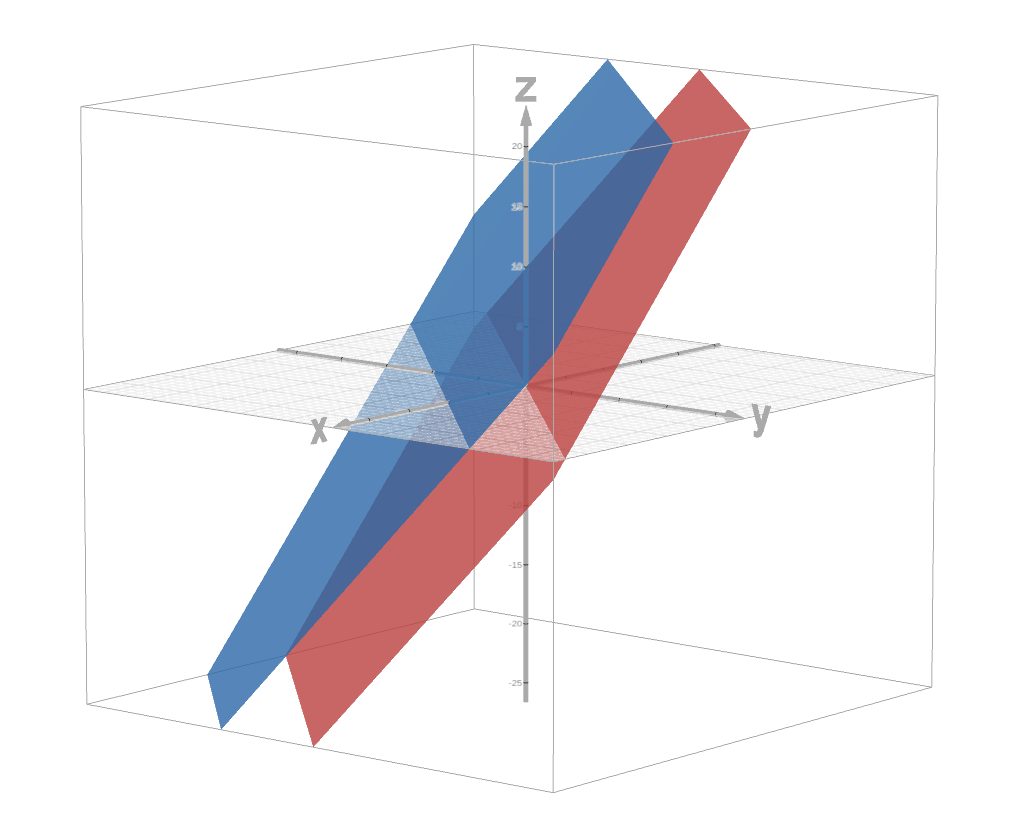
\includegraphics[scale=.18]{images/two-parallel-planes}
  \end{center}

  Or the three planes could intersect in a line, like the following picture,
  in which case there are infinitely many solutions (credit Noah C. for the
  observation and picture):
  \begin{center}
    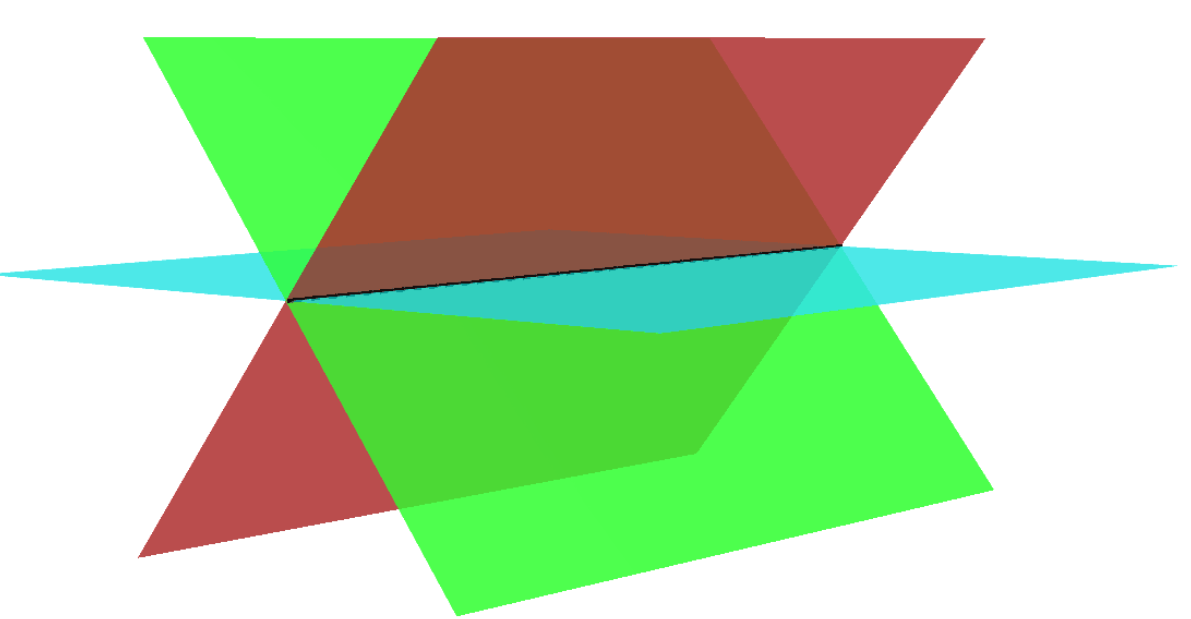
\includegraphics[scale=.18]{images/three-planes-intersect-in-a-line}
  \end{center}
  

  
  There are other ways that three planes could intersect as well, but the
  trichotomy stated earlier always holds: their intersection either constists
  of (1) exactly one point, (2) infinitely many points, or (3) zero points.
\end{example}

We've seen in this lecture that for systems of linear equations with two
variables, the solutions are the intersection of lines. For systems of linear
equations with three variables, the solutions are the intersections of planes.
... And for systems with $n>3$ variables, the solutions are the intersections
of hyperplanes.

\newpage

\section{2025-08-29 | Week 01 | Lecture 03}
\textit{This lecture is based on section 1.1 in the textbook}

\begin{center}
  \begin{tcolorbox}[width=0.9\textwidth, colback=white, colframe=black]
    \textit{\textbf{The nexus question of this lecture:} How can
      we solve a linear system without resorting to substitution?}
  \end{tcolorbox}
\end{center}

Recall in the boat example (\cref{ex:a-first-example-linear-system-equations}),
we had the system
\begin{equation*}
  \left\{ \begin{array}{l@{}l} x+y=12 \\ x-y=8 \end{array}\right.
\end{equation*}
And we could solve this using subsitution. Another thing we could have done,
would be to add the second equation to the first, giving us a new, simpler but
equivalent system:
\begin{equation*}
  \left\{ \begin{array}{l@{}l} 2x=20 \\ x-y=8 \end{array}\right.
\end{equation*}
Then divide the firs equation by two
\begin{equation*}
  \left\{ \begin{array}{l@{}l} x=10 \\ x-y=8 \end{array}\right.
\end{equation*}
Then subtract the first equation from the second:
\begin{equation*}
  \left\{ \begin{array}{l@{}l} x=10 \\ -y=-2 \end{array}\right.
\end{equation*}
Then multiply the second equation by $-1$
\begin{equation*}
  \left\{ \begin{array}{l@{}l} x=10 \\ y=2 \end{array}\right.
\end{equation*}
And tada! We have found our solution without doing substitution. But this
example was very simple, so maybe it's special and we can't always do this
sort of thing? Actually, we can. In the rest of the lecture, I'll try to
formalize these sorts of steps we used here and apply them to a more
complicated problem.

The reason I'm doing this is because, in the next lecture, I will begin to
present \demph{Gauss-Jordan elimination} (aka \demph{row reduction}), a
general method which can be used to find the solutions of any system of linear
equation which does not use substitution. For now, the we will work out an
example which motivates the main ideas that will be used by Gauss-Jordan
elimination.

\subsection{Solving a linear system using via simplifying transformations}

\begin{example}[Solving a linear system with elementary operations]
  \label{ex:solving-linear-system-with-elementary-operations}
  Suppose we wish to solve the following system:
  \begin{equation}
    \label{eq:elementary-operation-elimination-example}
    \left\{
      \begin{alignedat}{4}
        &x &{}\;-\; y &{}\;+\; &z{}&= &0 & \quad(E_{1}) \\ 
        2&x&{}\;-\; 3y&{}+\; 4&z{}&= -&2 & \quad(E_{2})\\
        -2&x&{}\;-\; y&{}\;+\; &z {}&= &7& \quad(E_{3})
      \end{alignedat}
    \right.
  \end{equation}
  This system has 3 equations, labeled $E_{1},E_{2},E_{3}$, and 3 variables
  $x,y$ and $z$. Suppose that we know ahead of time that this system has a
  unique solution (we showed this graphically in
  \cref{ex:system-with-three-variables}). Then, in principle, we could solve
  this using substitution, but that would suck. Instead, I will illustrate an
  approach in which we iteratively transform this linear system into
  successively simpler systems until we get to a point where the solution is
  obvious.

  To do this, we will play a game where there are three `moves' available to
  us. The three moves are:
  \begin{enumerate}
    \item Interchange two equations in the system.
    \item Multiply an equation by a nonzero number.
    \item Replace an equation by itself plus a multiple of another equation.
  \end{enumerate}
  These moves are called \demph{elementary operations}, and if we use them
  intelligently, they will allow us to transform the linear system into a
  simpler system.

  Two systems of equations are said to be \demph{equivalent} if they have the
  same solutions. Applying elementary operations always results in an
  equivalent system. Our goal will be to use some combination of elementary
  operations to produce a system of the form
  \begin{equation*}
    \left\{
      \begin{array}{l@{}l}
        x   &= *\\
        y &= *\\
        z &= *\\
      \end{array}\right.
  \end{equation*}
  where each $*$ is a constant which we will have computed. This will be our
  solution to the linear system \eqref{eq:elementary-operation-elimination-example},
  because the two systems will be equivalent.

  First, let's apply operation 3: specifically, by replacing $E_{2}$ with
  $E_{2} - 2E_{1}$:

\begin{equation*}
  \left\{
    \begin{alignedat}{4}
      &x &{}\;-\; y &{}\;+\; &z{}&= &0 \\
      & &{}\;-\; y&{}+\; 2&z{}&= -&2 \\
      -2&x&{}\;-\; y&{}\;+\; &z {}&= &7
    \end{alignedat}
  \right.
\end{equation*}
We have eliminated the $x$ from the second equation, yielding a simpler
system. Let's keep doing this. To eliminate $x$ from equation 3, let's apply
operation 3 again: This time, replace $E_{3}$ with $E_{3}+2 E_{1}$:
\begin{equation*}
  \left\{
    \begin{alignedat}{4}
      &x &{}\;-\; y &{}\;+\; &z{}&= &0 \\
      & &{}\;-\; y&{}+\; 2&z{}&= -&2 \\
      & &{}\; \; -3y&{}\;+\; 3&z {}&= &7
    \end{alignedat}
  \right.
\end{equation*}

Apply operation 3, replace $E_{1}$ with $E_{1}-E_{2}$. This will allow us to
eliminate $y$ from $E_{1}$:

\begin{equation*}
  \left\{
    \begin{alignedat}{4}
      &x &{}\;\;  &{}\;\; -&z{}&= &2 \\
      & &{}\;-\; y&{}+\; 2&z{}&= -&2 \\
      & &{}\; \; -3y&{}\;+\; 3&z {}&= &7
    \end{alignedat}
  \right.
\end{equation*}

Apply operation 3, replace $E_{3}$ with $E_{3}-3E_{2}$. This will allow us to
eliminate $y$ from $E_{3}$:
\begin{equation*}
  \left\{
    \begin{alignedat}{4}
      &x &{}\;\;  &{}\;\; -&z{}&= &2 \\
      & &{}\;-\; y&{}+\; 2&z{}&= -&2 \\
      & &{}\; \; &{}\;-\; 3&z {}&= &13
    \end{alignedat}
  \right.
\end{equation*}
Apply operation 2 twice: multiply both the first and second equations by $3$:
\begin{equation*}
  \left\{
    \begin{alignedat}{3}
      3x&   &{}\;\; -3&z{}= 6 \\
        & {}\;-\; 3y&{}\;+6&z{}= -6 \\
        & {}\; \; &{}\;\;- 3&z = 13
    \end{alignedat}
  \right.
\end{equation*}
Apply operation 3, twice. First, replace $E_{1}$ with $E_{1}-E_{3}$. Then
replace $E_{2}$ with $E_{2}+2E_{3}$. Doing both of these, we get:
\begin{equation*}
  \left\{
    \begin{alignedat}{3}
      3x \quad& &  & =&{} -7 \\
              & &-3y \quad \quad& =&{} 20 \\
              & & -3z& =&{} 13
    \end{alignedat}
  \right.
\end{equation*}
Apply operation $2$ by multiplying the first equation by $1/3$. Then multiply
the second and third equations both by $-1/3$:
\begin{equation*}
  \left\{
    \begin{alignedat}{3}
      x \quad& &  & =&{} -7/3 \\
             & &y \quad \quad& =&{} -20/3 \\
             & &z& =&{} -13/3
    \end{alignedat}
  \right.
\end{equation*}
This is the solution to the original equation. We have used elementary
operatons to reduce our original linear system
\cref{eq:elementary-operation-elimination-example} to the above system, which
equivalent to the original system.

While solving this system was still a lot of (tedious) work, it was still
probably simpler than doing substitution.
\end{example}

\subsection{Representing a linear system as an augmented matrix}
In the procedure presented in
\cref{ex:solving-linear-system-with-elementary-operations}, we didn't really
need to track the variables, only the \textit{coefficients} and the
\textit{quantities on the right hand sides} of the equations. Instead of
working with the equations directly, it will be simpler to work with the
following matrix, called the \demph{augmented matrix} corresponding go
\cref{eq:elementary-operation-elimination-example}:
\begin{equation*}
  \begin{augmentedmatrix}{ccc|c}
    1& -1& 1& 0 \\
    2& -3& 4& -2 \\
    -2& -1& 1& 7
  \end{augmentedmatrix}.
\end{equation*}
Comparing this with system \eqref{eq:elementary-operation-elimination-example}, it becomes
clear that the augmented matrix was obtained essentially by just erasing the
variables $x,y,$ and $z$ in \eqref{eq:elementary-operation-elimination-example}, and
then placing what remains into an array. We also drew a vertical line to the
separate the left- and right-hand sides of the equations. Inside the augmented
matrix, the $3\times 3$ submatrix  of coefficients
\begin{equation*}
  \begin{bmatrix}
    1& -1& 1\\
    2& -3& 4\\
    -2& -1& 1
  \end{bmatrix}
\end{equation*}
is called the \demph{coefficient matrix} of the system. 

More precise definitions are as follows:

\begin{definition}[Augmented Matrix]
  Given a linear system of the form \eqref{eq:defn-system-of-linear-equations},
  the \demph{augmented matrix} is
  \begin{equation*}
    \begin{augmentedmatrix}{cccc|c}
      a_{11}&a_{12}&\ldots& a_{1n}& b_{1}\\
      a_{21}&a_{22}&\ldots& a_{2n}& b_{2}\\
      \vdots &\vdots & &\vdots &\vdots \\
      a_{m1}&a_{m2}&\ldots& a_{mn}& b_{m}
    \end{augmentedmatrix}
  \end{equation*}
  and the \demph{coefficient matrix} is the matrix
  \begin{equation*}
    \begin{bmatrix}
      a_{11}&a_{12}&\ldots& a_{1n}\\
      a_{21}&a_{22}&\ldots& a_{2n}\\
      \vdots&\vdots & &\vdots \\
      a_{m1}&a_{m2}&\ldots& a_{mn}
    \end{bmatrix}.
  \end{equation*}
\end{definition}

This is our first application of 
\newpage
\section{2025-09-03 | Week 02 | Lecture 04}

\begin{center}
  \begin{tcolorbox}[width=0.9\textwidth, colback=white, colframe=black]
    \textit{\textbf{The nexus question of this lecture:} What is Gauss-Jordan
      elimination (aka: row reduction) and how do we use it to solve linear systems?}
  \end{tcolorbox}
\end{center}

Now I will present \demph{Gauss-Jordan elimination}. This is also called
\demph{Gaussian elimination}, or more commonly, \demph{row reduction}. I will
illustrate it by means of an example.

\subsection{Using row reduction to solve a linear system with a unique solution}
Suppose we wish to solve
\begin{equation}\label{eq:Gauss-Jordan-elimination-example}
  \left\{
    \begin{alignedat}{4}
      &x &{}\;-\; y &{}\;+\; &z{}&= &0 \\
      & &{}\;-\; y&{}+\; 2&z{}&= -&2 \\
      -2&x&{}\;-\; y&{}\;+\; &z {}&= &7
    \end{alignedat}
  \right.
\end{equation}

\Fl{Steps:} We initialize the algorithm by setting up an \demph{augmented
  matrix} corresponding to the system. For the system in
\eqref{eq:Gauss-Jordan-elimination-example}, the augmented matrix is
\begin{equation*}
  \begin{augmentedmatrix}{ccc|c}
    1& -1& 1& 0 \\
    2& -3& 4& -2 \\
    -2& -1& 1& 7
  \end{augmentedmatrix}.
\end{equation*}
\begin{itemize}
  \item The matrix to the left of the vertical row is the \demph{coefficient matrix.}
  \item A line of numbers going from left to right is called a \demph{row} of
  the matrix. A line of numbers going down the matrix is a \demph{column.}
\end{itemize}
Gauss-Jordan elimination is like a game where the player has three possible
moves, called \demph{row operations}.
\begin{enumerate}
  \item Interchange two rows.
  \item Multiply a row by a nonzero number.
  \item Replace a row by itself plus a multiple of another row.
\end{enumerate}
The player does row operations with the \textbf{goal} of making the diagonal
entries of the coefficient matrix 1's and making as many of the other numbers
zero, if possible. Here are the row operations for this example:
\begin{equation*}
  \phantom{ \overset{R_{2}-2R_{1}\to R_{2}}{\longrightarrow}}
  \begin{augmentedmatrix}{ccc|c}
    1& -1& 1& 0 \\
    2& -3& 4& -2 \\
    -2& -1& 1& 7
  \end{augmentedmatrix}
  \overset{R_{2}-2R_{1}\to R_{2}}{\longrightarrow}
  \begin{augmentedmatrix}{ccc|c}
    1& -1& 1& 0 \\
    \mathbf{0}& \mathbf{-1}& \mathbf{2}& \mathbf{-2} \\
    -2& -1& 1& 7
  \end{augmentedmatrix}
  \overset{R_{3}+2R_{1} \to R_{3}}{\longrightarrow}
  \begin{augmentedmatrix}{ccc|c}
    1& -1& 1& 0 \\
    0& -1& 2& -2 \\
    \mathbf{0}& \mathbf{-3}& \mathbf{3}& \mathbf{7}
  \end{augmentedmatrix}
\end{equation*}
\begin{equation*}
  \overset{R_{1}-R_{2} \to R_{1}}{\longrightarrow}
  \begin{augmentedmatrix}{ccc|c}
    \mathbf{1}& \mathbf{0}& \mathbf{-1}& \mathbf{2} \\
    0& -1& 2& -2 \\
    0& -3& 3& 7
  \end{augmentedmatrix}
  \overset{R_{3}-3R_{2} \to R_{3}}{\longrightarrow}
  \begin{augmentedmatrix}{ccc|c}
    1& 0& -1& 2 \\
    0& -1& 2& -2 \\
    \mathbf{0}& \mathbf{0}& \mathbf{-3}& \mathbf{13}
  \end{augmentedmatrix}
  \overset{(-1)\cdot R_{2} \to R_{2}}{\longrightarrow}
  \begin{augmentedmatrix}{ccc|c}
    1& 0& -1& 2 \\
    \mathbf{0}& \mathbf{1}& \mathbf{-2}& \mathbf{2} \\
    0& 0& -3& 13
  \end{augmentedmatrix}
\end{equation*}
\begin{equation*}
  \overset{(-\frac{1}{3})\cdot R_{3} \to R_{3}}{\longrightarrow}
  \begin{augmentedmatrix}{ccc|c}
    1& 0& -1& 2 \\
    0& 1& -2& 2 \\
    \mathbf{0}& \mathbf{0}& \mathbf{1}& \mathbf{-13/3}
  \end{augmentedmatrix}
  \overset{R_{2}+2R_{3} \to R_{2}}{\longrightarrow}
  \begin{augmentedmatrix}{ccc|c}
    1& 0& -1& 2 \\
    \mathbf{0}& \mathbf{1}& \mathbf{0}& \mathbf{-20/3} \\
    0& 0& 1& -13/3
  \end{augmentedmatrix}
  \overset{R_{1}+R_{3} \to R_{1}}{\longrightarrow}
  \begin{augmentedmatrix}{ccc|c}
    \mathbf{1}& \mathbf{0}& \mathbf{0}& \mathbf{-7/3} \\
    0& 1& 0& -20/3 \\
    0& 0& 1& -13/3
  \end{augmentedmatrix}
\end{equation*}
We now convert the augmented matrix back to a system of linear equations:
\begin{equation*}
  \left\{
    \begin{alignedat}{4}
      &1x &{}\;-\; 0y &{}\;+\; &0z{}&= -&7/3 \\
      &0x&{}\;-\; 1y&{}\;+\; &0z{}&= -&20/3 \\
      &0x&{}\;-\; 0y&{}\;+\; &1z {}&= -&13/3
    \end{alignedat}
  \right.
\end{equation*}
or more simply,
\begin{align*}
  x &= -7/3\\
  y &= -20/3\\
  z &= -13/3
\end{align*}
We can check that this is a solution to the original system of equations
\eqref{eq:Gauss-Jordan-elimination-example}.

\subsection{The goal when doing row reduction}
In the previoux example, we used row reduction Gauss-Jordan elimination to
solve a linear system. The example we did had a unique solution. When that
happens we can reduce the coefficient matrix to a matrix like
\begin{equation*}
  \begin{bmatrix}
    1&0&0\\
    0&1&0\\
    0&0&1\\
  \end{bmatrix}
\end{equation*}
possibly with one or more rows of zeros at the bottom. (It may be larger or
smaller depending on the number of equations and variables).

But in general, as we've seen, a linear system either has (1) one solution,
(2) no solutions, or (3) infinitely many solutions. And if cases (2) or (3)
happen, then we won't be able to do that. So we need to relax our ``goal''
when doing row reduction.

\textbf{Our new goal} is to reduce the coefficient matrix to \demph{reduced
  row-echelon form}, which in the case of a linear system with three equations
and three variables, means it should look like one of these
\begin{equation*}
  \begin{bmatrix}
    1&0&0\\
    0&1&0\\
    0&0&1\\
  \end{bmatrix}
  \quad \text{or} \quad
  \begin{bmatrix}
    1&0&\#\\
    0&1&\#\\
    0&0&0\\
  \end{bmatrix}
  \quad \text{or} \quad
  \begin{bmatrix}
    1&\#&\#\\
    0&0&0\\
    0&0&0\\
  \end{bmatrix}
\end{equation*}
where $\#$ denotes any arbitrary number.

\begin{definition}
  More precisely, a coefficient matrix
  \begin{equation*}
    \begin{bmatrix}
      a_{11}&a_{12}&\ldots& a_{1n}\\
      a_{21}&a_{22}&\ldots& a_{2n}\\
      \vdots&\vdots & &\vdots \\
      a_{m1}&a_{m2}&\ldots& a_{mn}
    \end{bmatrix}.
  \end{equation*}
  is said to be in \demph{reduced row echelon form} if
  \begin{enumerate}
    \item Any rows of zeros appear at the bottom
    \item The leftmost nonzero entry of all other rows equals 1 (the ``leading
    1's'')
    \item Each leading 1 of a nonzero row appears to the right of the leading
    row above it
    \item All the other entries of a column containing a leading $1$ are zero
  \end{enumerate}
\end{definition}
This definition is \textit{general}: it applies to any system with $m$ equations and
$n$ variables. The pattern will become natural once you've worked a few
(dozen?) examples.

\subsection{Using row reduction to solve a system with infitely many
solutions}

Here's an example which shows what happens when we try to solve a linear
system with infinitely many solutions:

\begin{example}[Using row reduction to solve a system with infitely many
  solutions]
  \label{ex:using-row-reduction-solve-system-with-infitely-many-solutions}
  We wish to solve the system
  \begin{equation*}
    \left\{ \begin{array}{l@{}l}
      \phantom{-}2x+3y-z\ &=3  \\
      -x-\phantom{2}y+3z\ &=0  \\
      \phantom{-}x+2y+2z\ &=3  \\
      \phantom{2x+3}y+5z\ &=3 
      \end{array}\right. 
  \end{equation*}

  This system has 4 equations and 3 variables. Each equation represents a
  plane. The solutions, if there are any, will be the intersection of these
  four planes. I've plotted the planes in Desmos:

  \begin{center}
    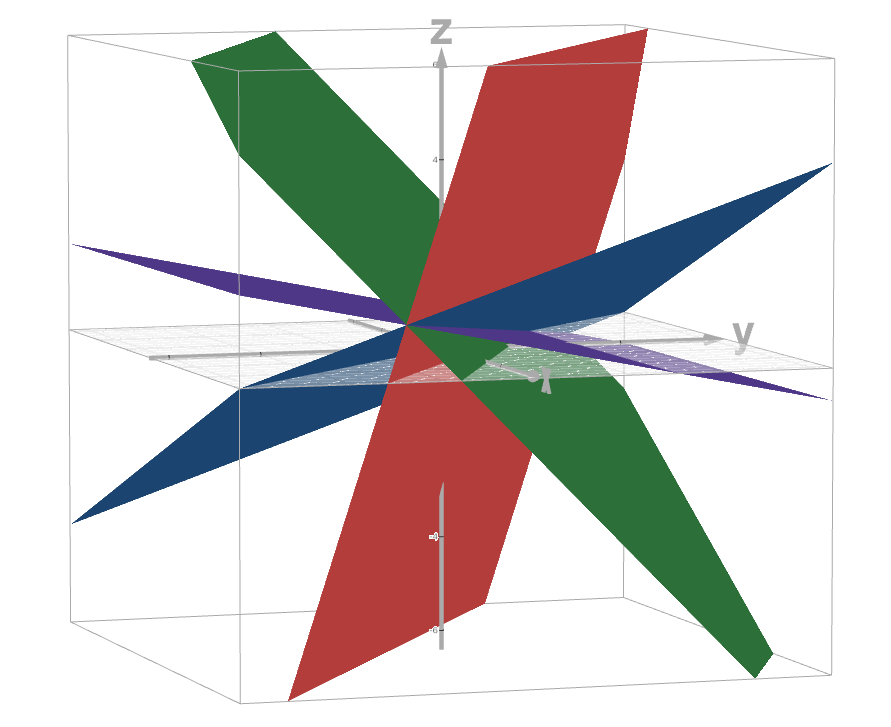
\includegraphics[scale=.2]{images/line-of-solutions}
  \end{center}
  It looks like the four planes intersect in a line. So we should expect
  infinitely many solutions.
  
  \Fl{Step 1.} Write down the augmented matrix of the system.

  \begin{equation*}
    \begin{augmentedmatrix}{ccc|c}
      2&3&-1&3\\
      -1&-1&3&0\\
      1&2&2&3\\
      0&1&5&3
    \end{augmentedmatrix}
  \end{equation*}

  \Fl{Step 2.} Do some combination or row reduction steps until the
  coefficient matrix is in reduced row echelon form. (This is Example 3 in the
  textbook, refer there for the steps.)
  
  \Fl{Step 3.} Our matrix is now in reduced row echelon form:
  \begin{equation*}
    \begin{augmentedmatrix}{ccc|c}
      1&0&-8&-3\\
      0&1&5&3\\
      0&0&0&0\\
      0&0&0&0
    \end{augmentedmatrix}
  \end{equation*}
  Let's convert it back into a linear system of equations:
  \begin{align*}
    x-8z&=-3\\
    y+5z&=3\\
    0&=0\\
    0&=0
  \end{align*}
  Therefore, we have
  \begin{equation}\label{eq:example-of-line-of-solutions}
    \left\{ \begin{array}{l@{}l} x=-3+8z \\ y=3-5z \end{array}\right.
  \end{equation}
  where $z$ is any real number. There are no restrictions on the value of $z$.
  Any choice of $z$ gives us a valid solution to our original system of
  equations. If $z=0$, we have the solution $(x,y,z)=(-3,3,0)$. If $z=1$, then
  we have the solution $(x,y,z)= (5,-2,1)$, and so forth.

  \textbf{Interpretation:} In this case, $z$ is called a \demph{free variable}
  and $x$ and $y$ are called \demph{dependent variables}. The solutions to the
  original linear system consist of all points on a line which cuts through
  3-dimensional space $\R^{3}$. \cref{eq:example-of-line-of-solutions} gives
  us a parametric equation of the line. The set of solutions is 1-dimensional,
  because it is a line.
\end{example}

We've covered two of the three cases. For the last case, we consider the
question \textit{what happens if we attempt to solve a linear system that has
  no solutions?}


\subsection{Using row reduction to attempt to solve a system with no
  solutions}
\begin{example}[Using row reduction to attempt to solve a system with no
  solutions]
  \label{ex:using-row-reduction-attempt-solve-system-with-no-solutions}
  Suppose we wish to solve the system
  \begin{align*}
    2x+y-z&=3\\
    -x-y+2z&=0\\
    -x-y+2z&=4\\
  \end{align*}
  Here's a plot of the planes:
  \begin{center}
    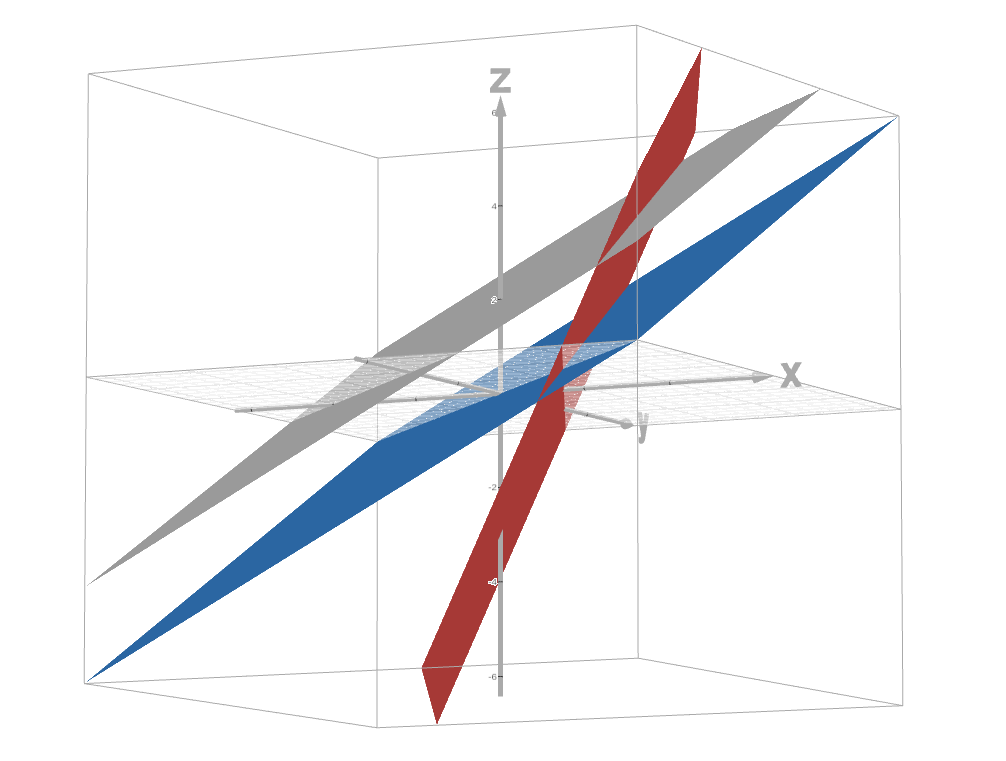
\includegraphics[scale=.2]{images/inconsistent-system}
  \end{center}
  Their intersection if the three planes is \textit{empty}: there is no point
  which lies on all three planes. So this system has no solution. What happens
  when we try to use row reduction? 

  \Fl{Step 1.} Write
  down the augmented matrix:
  \begin{equation*}
    \begin{augmentedmatrix}{ccc|c}
      2&1&-1&3\\
     -1&-1&2&0\\
      -1&-1&2&4
    \end{augmentedmatrix}
  \end{equation*}

  \Fl{Step 2.} Do row reduction to get to reduced row echelon form (I'm
  skipping steps here):
  \begin{equation*}
    \begin{augmentedmatrix}{ccc|c}
      1&0&1&3\\
      1&-1&3&3\\
      0&0&0&4
    \end{augmentedmatrix}
  \end{equation*}

  \Fl{Step 3.} Convert back to a linear system:
  \begin{equation*}
    \left\{ \begin{array}{l@{}l}
        x\phantom{-y3\ }+z&=3\\
        x-y+3z\ &=3\\
        0&=4 \\  \end{array}\right.
  \end{equation*}
  The last equation is never true, no matter what values we choose for $x,y$
  and $z$. So the system has no solution
\end{example}
\subsection{Notes and resources for learning row reduction}

\Fl{NOTE:} I'm not going to do a lot of examples of row reduction because it's
so time consuming that it's not a great use of lecture time. So I expect you
to teach yourself how to do row reduction. If you want to see more examples,
some good online videos are
\begin{center}
  \url{https://www.youtube.com/watch?v=OP2aQUOevhI}
  
  \url{https://www.youtube.com/watch?v=eDb6iugi6Uk}
\end{center}

There are also some nice online tools to help with row reduction, for example:

\begin{center}
  \url{https://textbooks.math.gatech.edu/ila/demos/rrinter.html}

  \url{https://www.math.odu.edu/~bogacki/cgi-bin/lat.cgi?c=roc}
\end{center}

\fl{General advice:}
\begin{enumerate}
  \item Of course I'm going to ask you to row-reduce matrices on your exams,
  and for that you'll need to be able to do it by hand, without a calculator.
  \item Write down all your steps, including a new matrix at every step in an
  organized way.
  \item Use the notation $R_{i}\leftrightarrow R_{j}$ to indicate a swap of
  rows $i$ and $j$; $cR_{i}\to R_{i}$ to indicate a multiplication of row $i$
  by a constant $c$; and, $R_{i}+cR_{j}\to R_{i}$ to indicate that you've
  added $c$ times row $j$ to row $i$.
  \item Work left to right, top to bottom. Start by making the top left entry
  1. Then use it to make all the numbers below it zero. Then go to the second
  column, second row, and make that 1. Then make everything beneath it zero.
  Etc.
\end{enumerate}

\newpage
\section{2025-09-05 | Week 02 | Lecture 05}

\begin{center}
  \begin{tcolorbox}[width=0.9\textwidth, colback=white, colframe=black]
    \textit{\textbf{The nexus question of this lecture:} What is a matrix, and
      what are the fundamental algebraic operations we can do with it?}
  \end{tcolorbox}
\end{center}

\textit{This lecture is based on section 1.2 in the textbook.}

\subsection{Matrices and matrix notation}

A \demph{matrix} is a rectangular array of objects, usually numbers, which are
called \demph{entries}. If the number of rows and the number of columns are
equal, the matrix is said to be a \demph{square matrix}.

For example,
\begin{equation*}
  \begin{bmatrix}
    1&0&3\\
    2&5&-3
  \end{bmatrix}
  \quad \text{or} \quad
  \underbrace{\begin{bmatrix}
    1&0&-7&5
  \end{bmatrix}}_{a \demph{row vector}}
  \quad \text{or} \quad
  \underbrace{\begin{bmatrix}
    1\\4\\0
  \end{bmatrix}}_{a \demph{column vector}}
  \quad \text{or} \quad
  \begin{bmatrix}
    1&0\\
    0&-1
  \end{bmatrix}
\end{equation*}
A matrix with $m$ rows and $n$ columns takes the form
\begin{equation*}
  A=
  \begin{bmatrix}
    a_{11}&a_{12}&\ldots& a_{1n}\\
    a_{21}&a_{22}&\ldots& a_{2n}\\
    \vdots&\vdots & &\vdots \\
    a_{m1}&a_{m2}&\ldots& a_{mn}
  \end{bmatrix}.
\end{equation*}
Such a matrix is said to be an \demph{$m\times n$ matrix}. The pair $(m,n)$
is called the \demph{dimensions} of the matrix (i.e., the number of rows and
number of columns). If $m=n$, then the matrix is said to be a \demph{square matrix}.

The set of all $m\times n$ matrices with real entries is denoted
\begin{equation*}
  M_{m\times n}(\R)
\end{equation*}
For example, in set notation
\begin{equation*}
  M_{2\times 3}(\R) = \left\{
    \begin{bmatrix}
      a_{11}&a_{12}&a_{13}\\
      a_{21}&a_{22}&a_{23}\\
    \end{bmatrix}
    :
    a_{11},a_{12},a_{13},a_{21},a_{22},a_{23}\in \R 
  \right\} 
\end{equation*}

\begin{notation}
  It is common to denote a matrix compactly using the notation
  \begin{equation*}
    A=[a_{ij}]
    \quad \text{or} \quad
    A=(a_{ij})
  \end{equation*}
  To denote the entry at row $i$, column $j$, we write either
  \begin{equation*}
    \text{ent}_{ij}(A)
    \quad \text{or more simply,} \quad
    a_{ij}
  \end{equation*}
  For example, if
  \begin{equation*}
    A = (a_{ij}) = \begin{bmatrix}
      -1&2&1\\
      5&4&-9\\
      3&-4&7
    \end{bmatrix}
  \end{equation*}
  then $a_{23} = \text{ent}_{23}(A) = -9$, and $a_{21}=\text{ent}_{21}=5$.
\end{notation}

Vectors are a special case of matrices. An $n$-dimensonal vector is an
$n\times 1$ matrices (a column matrix, typically).

\subsection{Matrix operations: scaling, addition and multiplication}
We can \demph{multiply matrices by a scalar}, in the obvious way:
$10\times \begin{bmatrix}
  3&4\\
  -2&0
\end{bmatrix}
=
\begin{bmatrix}
  30&40\\
  -20&0
\end{bmatrix}$.

\noindent We can \demph{add matrices}, also in the obvious way:
\begin{equation*}
  \begin{bmatrix}
    3&4\\
    -2&0
  \end{bmatrix}
  +
  \begin{bmatrix}
    1&5\\
    2&10
  \end{bmatrix}
  =
  \begin{bmatrix}
    4&9\\
    0&10
  \end{bmatrix}.
\end{equation*}
But note that we can only add two matrices if they have the same dimensons:
\begin{equation*}
  \begin{bmatrix}
    5&2\\
    -2&-1
  \end{bmatrix}
  +
  \begin{bmatrix}
    -1&10\\
    4&7\\
    2&5
  \end{bmatrix}
  = \text{ undefined}.
\end{equation*}
We can also \textbf{multiply} matrices, but before defining matrix
multiplication, it will be helpful to recall the notion of dot product.
Suppose we have two vectors of the same length:
\begin{equation*}
  X =
  \begin{bmatrix}
    x_{1}&x_{2}&\cdots&x_{n}
  \end{bmatrix}
  \quad \text{and} \quad
  Y =
  \begin{bmatrix}
    y_{1}&y_{2}&\cdots&y_{n}
  \end{bmatrix},
\end{equation*}
then the \demph{dot product} of $X$ and $Y$, denoted $X\cdot Y$, is
\begin{align*}
  X\cdot Y 
  &= x_{1}y_{1}+ x_{2}y_{2}+\ldots+x_{n}y_{n} = \sum_{i=1}^{n}x_{i}y_{i}.
\end{align*}
\demph{Matrix multiplication} is defined in the following way:


\begin{tcolorbox}[colframe=black, colback=gray!5, arc=2mm, boxrule=0.8pt,
  breakable, title=Matrix Multiplication,   coltitle=black,colbacktitle=black!10]
  If $A=(a_{ij})$ is a $p\times n$ matrix and $B=(b_{ij})$ is an $n\times q$
  matrix, then we can can think of $A$ and $B$ as
  \newcommand*{\vertbar}{\rule[-1ex]{0.5pt}{2.5ex}}
  \newcommand*{\horzbar}{\,\rule[.5ex]{2.5ex}{0.5pt}\,}
  \begin{equation*}
    A =
    \left[\begin{array}{c}
        \horzbar  A_{1}  \horzbar \\
        \horzbar  A_{2}  \horzbar \\
        \vdots             \\
        \horzbar  A_{p} \horzbar
      \end{array}\right]
    \quad \text{and} \quad
    B = 
    \left[
      \begin{array}{cccc}
        \vertbar & \vertbar &        & \vertbar \\
        B_{1}    & B_{2}    & \ldots & B_{q}    \\
        \vertbar & \vertbar &        & \vertbar 
      \end{array}
    \right]
  \end{equation*}
  where $A_{1},\ldots,A_{p}$ are the $1\times n$ row vectors
  \begin{equation*}
    A_{i} =
    \begin{bmatrix}
      a_{i1}& a_{i2}& \cdots & a_{in}
    \end{bmatrix}
    \quad (i=1,\ldots,p)
  \end{equation*}
  and $B_{1},\ldots,B_{q}$ are $n\times 1$ column vectors:
  \begin{equation*}
    B_{j} =
    \begin{bmatrix}
      b_{1j}\\b_{2j}\\\vdots\\b_{nj}
    \end{bmatrix}
    \quad (j=1,2,\ldots,q)
  \end{equation*}
Then the product $P=AB$ is a $p\times q$ matrix $P=(p_{ij})$, whose entries are
\begin{align*}
  p_{ij} 
  &= A_{i}\cdot B_{j} \\
  &= \sum_{k=1}^{n}a_{ik}b_{kj}.
\end{align*}
\end{tcolorbox}

For example,
\begin{equation*}
  \begin{bmatrix}
    1&2\\
    3&4
  \end{bmatrix}
  \begin{bmatrix}
    5&6\\
    7&8
  \end{bmatrix}
  =
  \begin{bmatrix}
    1\cdot 5+2\cdot7 & 1\cdot 6 + 2\cdot8\\
    3\cdot 5+4\cdot7 & 3\cdot 6 + 4\cdot8
  \end{bmatrix}
  =
  \begin{bmatrix}
    19&22\\
    43&50
  \end{bmatrix}
\end{equation*}

\Fl{Dimensionality requirement for matrix multiplication:} we can only multiply
two matrices if their dimensions match in the right way. If $A$ is a
$p\times n$ matrix, and $B$ is an $\tilde{n} \times q$ matrix, then the
product $AB$ is defined if and only if $n=\tilde{n}$. That is,
\begin{equation*}
  AB \text{ is } \left\{ \begin{array}{l@{\quad \text{if }\quad}l} \text{a $p\times q$ matrix} & n=\tilde{n} \\
      \text{undefined}& n\neq \tilde{n} \end{array}\right.
\end{equation*}

\Fl{Properties of matrix multiplication:} Perhaps surprisingly, despite
matrix multiplication's complicated definition, it nonetheless behaves sort of
like regular multiplication in that the \demph{associative property} and
\demph{distributed property} both hold. That is,
\begin{equation*}
  ABC = (AB)C = A(BC) \quad \text{(associative property)}
\end{equation*}
and
\begin{gather*}
  A(B+C) = AB+BC \quad \text{(left distributive property)}\\
  (B+C)A = BA+CA \quad \text{(right distributive property)}
\end{gather*}

It's not obvious why the properties always hold; they require proof. For now,
we will take them as a given.


\subsection{Special classes of matrices }

\subsubsection{Diagonal matrices}
If $A=(a_{ij})$ is a square (i.e., $n\times n$) matrix, then the entries
$a_{11},a_{22},a_{33},\ldots,a_{nn}$ are called the \demph{diagonal
  entries}. A square matrix of the form
\begin{equation*}
  A =\begin{bmatrix}
    a_{11}&0&0&\ldots& 0\\
    0&a_{22}&0&\ldots& 0\\
    0&0&a_{33}&\ldots& 0\\
    \vdots&\vdots & &\ddots \\
    0&0&0&\ldots& a_{nn}
  \end{bmatrix}.
\end{equation*}
is called a \demph{diagonal} matrix, and the notation used for such matrices
is $A=\diag(a_{11},\ldots,a_{nn})$.

\subsubsection{Identity matrix}
An \demph{identity matrix} is a diagonal matrix with 1's on its diagonal (and
0's everywhere else). For example,
\begin{equation*}
  \begin{bmatrix}
    1&0\\
    0&1
  \end{bmatrix}
  \quad \text{or} \quad
  \begin{bmatrix}
    1&0&0\\
    0&1&0\\
    0&0&1
  \end{bmatrix}
  \quad \text{or} \quad
  \begin{bmatrix}
    1&0&0&0\\
    0&1&0&0\\
    0&0&1&0\\
    0&0&0&1\\
  \end{bmatrix}
  \quad \text{et cetera}
\end{equation*}
Identity matrices are always square. The notation for an $n\times n$
identity matrix is $I_{n}$, or more simply $I$.

An identity matrix has the property that when you multiply it by another matrix, it doesn't
change the other matrix. For example,
\begin{equation*}
  \begin{bmatrix}
    5&6\\
    2&7
  \end{bmatrix}
  \begin{bmatrix}
    1&0\\
    0&1
  \end{bmatrix}
  =
  \begin{bmatrix}
    5&6\\
    2&7
  \end{bmatrix}
\end{equation*}
It's like multiplying a number by 1.

\subsubsection{Zero matrices}

A matrix whose entries are all zeros is called a \demph{zero matrix}, like
\begin{equation*}
  \begin{bmatrix}
    0&0\\
    0&0
  \end{bmatrix}
  \quad \text{or} \quad
  \begin{bmatrix}
    0&0&0\\
    0&0&0\\
    0&0&0
  \end{bmatrix}
  \quad \text{or} \quad
  \begin{bmatrix}
    0&0&0\\
    0&0&0\\
  \end{bmatrix}
  \quad \text{et cetera}
\end{equation*}
The book uses the notation $\mathbf{O}_{m\times n}$ to denote an $m\times n$
zero matrix, or sometimes even just $\mathbf{O}$.

\newpage
\section{2025-09-08 | Week 03 | Lecture 06}

\begin{center}
  \begin{tcolorbox}[width=0.9\textwidth, colback=white, colframe=black]
    \textit{\textbf{The nexus question of this lecture:} How do we encode a
      linear system using matrices? And once thus encoded, what can we say
      about the solutions to the linear system just by looking at the matrix?}
  \end{tcolorbox}
\end{center}

\textit{This lecture is based on sections 1.2 and 1.3 of the textbook.} 


\subsection{Inverting matrices}
We begin this lecture by introducing the idea of a matrix inverse, which we
will use to help answer the main question of the lecture.

Recall that the identity matrix is a matrix of the form
\begin{equation*}
  \begin{bmatrix}
    1&0\\
    0&1
  \end{bmatrix}
  \quad \text{or} \quad
  \begin{bmatrix}
    1&0&0\\
    0&1&0\\
    0&0&1
  \end{bmatrix}
  \quad \text{or} \quad
  \begin{bmatrix}
    1&0&0&0\\
    0&1&0&0\\
    0&0&1&0\\
    0&0&0&1\\
  \end{bmatrix}
  \quad \text{et cetera}
\end{equation*}
and we usually denote an identity matrix by the letter $I_{n}$ (or just $I$ if
the dimensions are clear from context). Such a matrix behaves like the number
$1$, in the sense that $AI=A$ and $IA=A$ for any matrix $A$.

Every nonzero number $a$ has an inverse $a^{-1}=\frac{1}{a}$ such that
\begin{equation*}
  a\cdot a^{-1} = a^{-1}a = 1.
\end{equation*}
It would natural to conjecture that every nonzero matrix $A$ also has an
inverse $A^{-1}$ such that
\begin{equation*}
  AA^{-1}=A^{-1}A = I
\end{equation*}
In fact, this conjecture is false: we cannot do this with every matrix, but
sometimes we can.

To be precise, if two matrices satisfy the property that $AB=BA=I$, then they
are said to be \demph{inverses}. In this case, we write $B=A^{-1}$ (which
doesn't mean $1/A$). This is analogous to when we multiply two numbers like
$3\cdot \frac{1}{3}= \frac{1}{3}\cdot 3=1$.



\begin{example}[Matrix inverses]
  An example are the matrices
  \begin{equation*}
    A =
    \begin{bmatrix}
      1&2\\
      3&5
    \end{bmatrix}
    \quad \text{and} \quad
    B =
    \begin{bmatrix}
      -5&2\\
      3&-1
    \end{bmatrix}
  \end{equation*}
  Because
  \begin{align*}
    AB
    &=
      \begin{bmatrix}
        1&2\\
        3&5
      \end{bmatrix}
           \begin{bmatrix}
             -5&2\\
             3&-1
           \end{bmatrix}
    \\
    &= 
      \begin{bmatrix}
        1(-5)+ 2\cdot 3 & 1\cdot2+2(-1)\\
        3(-5)+ 5\cdot 3 & 2\cdot2+5(-1))
      \end{bmatrix}
    \\
    &= 
      \begin{bmatrix}
        1&0\\
        0&1
      \end{bmatrix}\\
    &= I_{2}
  \end{align*}
  And similarly, $BA = I_{2}$. Therefor $A^{-1}=B$.
\end{example}

As noted, not every matrix has an inverse. A matrix that doesn't have an
inverse is called \demph{singular} or \demph{noninvertible}. A matrix that has
an inverse, is called \demph{nonsingular} or \demph{invertible}. Generally in
mathematics, ``singular'' means ``bad''.

Moreover, note that it is possible for $AB=I$ but $BA\neq I$, as the following
example shows.

\begin{example}
  Let
  \begin{equation*}
    A=\frac{1}{\sqrt{2}}\begin{bmatrix}
      1 & 1& 0 & 0\\
      0&0&1&1
    \end{bmatrix}
    \quad \text{and} \quad
    B=
    \frac{1}{\sqrt{2}}
    \begin{bmatrix}
      1 & 0\\
      1 & 0\\
      0&1\\
      0&1
    \end{bmatrix}
  \end{equation*}
  Then
  \begin{equation*}
    AB =
    \begin{bmatrix}
      1&0\\
      0&1
    \end{bmatrix}
    \quad \text{but} \quad 
    BA =
    \frac{1}{2}\begin{bmatrix}
      1&1&0&0\\
      1&1&0&0\\
      0&0&1&1\\
      0&0&1&1\\
    \end{bmatrix}
  \end{equation*}
\end{example}
Incidentally this example illustrates one imporant way that matrix multiplication is not like
multiplication of numbers.

\subsection{An aside about commutatitivity}
Consider two real numbers $a,b\in \R$. Then
\begin{equation*}
  ab = ba.
\end{equation*}
This property is called \demph{commutatitivity}. One way that matrix
multiplication differs from multiplication of real numbers is that if we
consider two matrices $A,B$, then it is usually not the case that $AB=BA$.
Whenever it is the case that $AB=BA$, we say that the matrices $A$ and $B$
\demph{commute}, but again, this usually doesn't happen. Here are some
examples:

\begin{example}[Commutativity and noncommutatitivity of matrix multiplication]
  Let
  \begin{equation*}
    A =
    \begin{bmatrix}
      1&1\\
      0&1
    \end{bmatrix},
    \quad
    B =
    \begin{bmatrix}
      2&3\\
      0&2
    \end{bmatrix}
    \quad \text{and} \quad
    C =
    \begin{bmatrix}
      2&0\\
      3&1
    \end{bmatrix}.
  \end{equation*}
  Direct computation shows that
  \begin{equation*}
    AB=BA =
    \begin{bmatrix}
      2&5\\
      0&2
    \end{bmatrix}.
  \end{equation*}
  In this case, we say that the matrices $A$ and $B$ commute.

  On the other hand, the matrices $A$ and $C$ do not commute because
  \begin{equation*}
    AC =
    \begin{bmatrix}
      5&1\\
      3&1
    \end{bmatrix}
    \quad \text{but} \quad
    CA =
    \begin{bmatrix}
      2&2\\
      3&4
    \end{bmatrix}
  \end{equation*}
  so $AC\neq CA$.
\end{example}


\subsection{Encoding a linear system via matrix equations}
In this section, we answer the first part of the main question of lecture.
Consider the $2\times 2$ linear system
\begin{gather*}
  3x_{1}+7x_{2}=5\\
  2x_{1}-6x_{2}=1
\end{gather*}
Using matrix multiplication, we can write this system as
\begin{equation*}
  \begin{bmatrix}
    3&7\\
    2&-6
  \end{bmatrix}
  \begin{bmatrix}
    x_{1}\\x_{2}
  \end{bmatrix}
  =
  \begin{bmatrix}
    5\\1
  \end{bmatrix}
\end{equation*}
In fact, we can do something similar with any linear system, as we now show:

Suppose we have any linear system, like this:
\begin{equation*}
  \left\{ \begin{array}{l@{}l}
      \ a_{11}x_{1}+a_{12}x_{2}+\ldots+a_{1n}x_{n} = b_{1} \\
      \ a_{21}x_{1}+a_{21}x_{2}+\ldots+a_{2n}x_{n} = b_{2} \\
      \hfill\vdots\hfill \\
      a_{m1}x_{1}+a_{m2}x_{2}+\ldots+a_{mn}x_{n} = b_{m}
    \end{array}\right.
\end{equation*}
Define the three matrices
\begin{equation*}
  A =
  \begin{bmatrix}
    a_{11}&a_{12}&\ldots& a_{1n}\\
    a_{21}&a_{22}&\ldots& a_{2n}\\
    \vdots&\vdots & &\vdots \\
    a_{m1}&a_{m2}&\ldots& a_{mn}
  \end{bmatrix},
  \quad
  X =
  \begin{bmatrix}
    x_{1}\\x_{2}\\\vdots\\x_{n}
  \end{bmatrix}
  \quad \text{and} \quad
  B =
  \begin{bmatrix}
    b_{1}\\b_{2}\\\vdots\\b_{m}
  \end{bmatrix}
\end{equation*}
Then we can represent the linear system compactly as the matrix equation
\begin{equation*}
  AX=B.
\end{equation*}
This answers the question \textit{``how can we encode a linear system using
  matrices?''} (It alsow provides us with the beginnings of an answer to the
question \textit{``why is matrix multiplication defined the way it is?''},
which is that matrix multiplication allows us to compactly represent linear
systems, though a more compelling answer to this question will come later in
the course.)

\subsection{What does \texorpdfstring{$A$}{A} tell us about
  the linear system \texorpdfstring{$AX=B$}{AX=B}?}
For the remainder of the lecture, we consider the question, \textit{``What can
  we tell about the solutions to the linear system $AX=B$, just by looking at
  the matrix $A$?''} It is not obvious that we should be able to tell anything
at all about the solutions just by looking at $A$---after all, that's, like
trying to says something about the solutions to a system of equations
\textit{by only looking at the left-hand sides of the equations.} 

Observe that if we know $A^{-1}$, then we can multiply both sides of this
equation on the left by
\begin{equation*}
  A^{-1}AX = A^{-1}B
\end{equation*}
which simplifies to
\begin{equation}
  \label{eq:inverse-solution-to-linear-equation}
  X = A^{-1}B.
\end{equation}
Thus, $X$ is the unique solution to our original system. This motivates the
following theorem:
\begin{theorem}
  \label{thm:unique-solution-invertibility}
  A linear system $AX=B$ with $n$ equations and $n$ variables has exactly one
  solution if and only if $A$ is invertible.
\end{theorem}

This theorem provides a partial answer to the main question of the lecture.
What is remarkable is that it says we don't need to know anything at all about
the vector $B$ to know whether the system has a unique solution. We only need
to know whether $A$ is singular or nonsingular. This hints a deeper structure
in linear algebra that we will explore more fully throughout this course.

As an aside, note that when doing computations, it is usually easier to solve
a linear system $AX=B$ directly using row reduction, rather than (1) finding
the inverse of $A$ and then (2) multiplying both sides by $A^{-1}$. So the
latter approach isn't recommended for solving a system of linear equations.
Just use row reduction.

We can actually push our answer to the lecture question a little bit further,
by drawing a connection with one of your homework problems (homework 1,
problem 3). In that problem, you showed that for the matrix $A=
\begin{bmatrix}
  a_{11}&a_{12}\\
  a_{21}&a_{22}
\end{bmatrix}
$, the linear system
\begin{equation*}
  AX=B
\end{equation*}
has a unique solution if and only if the determinant of $A$ (defined as
$a_{11}a_{22}-a_{12}a_{21}$) is nonzero. That is,
\begin{equation*}
  \text{determinant of $A$ is nonzero} \iff \text{ $AX=B$ has a unique solution }
\end{equation*}
Connecting this with \cref{thm:unique-solution-invertibility}, we have:
\begin{equation*}
  \text{determinant of $A$ is nonzero} \iff \text{ $AX=B$ has a unique solution} \iff
  \text{$A$ is invertible}
\end{equation*}
Putting it together, we have the following theorem, which gives us an answer
to the main question of the lecture:
\begin{theorem}
  \label{thm:key-theorem}
  Let $A$ be an $n\times n$ matrix. Then the following are equivalent:
  \begin{enumerate}[label=(\roman*.)]
    \item $A$ is invertible.
    \item The determinant of $A$ is nonzero.
    \item For any vector $B\in\R^{n}$ the linear system $AX=B$ has exactly one solution.
  \end{enumerate}
\end{theorem}
We haven't proved this theorem for all matrices; we've only shown that it
holds for $2\times 2$ matrices. In fact, it holds for all matries, as we'll
see later.


\newpage

\section{2025-09-10 | Week 03 | Lecture 07}

\textit{This lecture isn't really based on any textbook section, but sections
  1.5 and 1.6 cover determinants. Please read sections 1.3 and 1.4 for
  Friday.}

\begin{center}
  \begin{tcolorbox}[width=0.9\textwidth, colback=white, colframe=black]
    \textit{\textbf{The nexus question of this lecture:} What is a
      determinant, geometrically?}
  \end{tcolorbox}
\end{center}

\subsection{The determinant of  \texorpdfstring{$2\times 2$}{2\times2} matrix}

Recall that the determinant of a $2\times 2$ matrix is
defined as the quantity
\begin{equation*}
  \det \begin{bmatrix}
    a&b\\
    c&d
  \end{bmatrix} = ad-bc.
\end{equation*}
Later we'll see how to define determinants for $n\times n$ matrices, but for
this lecture I'm going to focus on the $2\times 2$ case in order to hopefully
demonstrate why you should even care about determinants at all.

\subsection{A matrix is a transformation of space}

Consider the $2\times 2$ matrix
\begin{equation*}
  A=\begin{bmatrix}
    3&1\\
    1&2
  \end{bmatrix}.
\end{equation*}

\subsubsection*{Preliminaries: Some elementary properties of \texorpdfstring{$A$}{A} }
Let us consider what this matrix does to the standard basis vectors $e_{1}=
\begin{bmatrix}
  1\\0
\end{bmatrix}
$
and $e_{2}=
\begin{bmatrix}
  0\\1
\end{bmatrix}
$:

\begin{equation*}
  Ae_{1}
  =
  \begin{bmatrix}
    3&1\\
    1&2
  \end{bmatrix}
  \begin{bmatrix}
    1\\0
  \end{bmatrix}
  =
  \begin{bmatrix}
    3\\1
  \end{bmatrix}
  \quad \text{and} \quad
  Ae_{2}
  =
  \begin{bmatrix}
    3&1\\
    1&2
  \end{bmatrix}
  \begin{bmatrix}
    0\\1
  \end{bmatrix}
  =
  \begin{bmatrix}
    1\\2
  \end{bmatrix}
\end{equation*}
In other words, multiplication by $A$ sends the vector $e_{1}$ to the vector
$\begin{bmatrix} 3\\1 \end{bmatrix}$. It sends the vector $e_{2}$ to
$\begin{bmatrix} 1\\2 \end{bmatrix}$.

Let's give these vectors names and compute some values that will be useful later:
\begin{equation*}
  u =
  \begin{bmatrix}
    3\\1
  \end{bmatrix}
  \quad \text{and} \quad
  v =
  \begin{bmatrix}
    1\\2
  \end{bmatrix}
\end{equation*}
\begin{itemize}
  \item The magnitudes of $u$ and $v$ are
  \begin{equation*}
    |u| = \sqrt{3^{2}+1^{2}} = \sqrt{10}
    \quad \text{and} \quad
    |v| = \sqrt{2^{2}+1^{2}} = \sqrt{5}
  \end{equation*}
  \item The cosine of angle $\theta$ between $u$ and $v$ can be computed using
  the dot product, by the formula
  \begin{equation*}
    u\cdot v = |u||v| \cos(\theta).
  \end{equation*}
  Doing the computation, we get
  \begin{equation}\label{eq:cosine-example}
    \cos(\theta) = \frac{1}{\sqrt{2}}.
  \end{equation}
\end{itemize}

\subsubsection*{The key idea}
Suppose we decided to multiply \textit{every} vector in the plane by the
matrix $\begin{bmatrix}
  3&1\\
  1&2
\end{bmatrix}$. In that case, we could conceive of the matrix transforming
space (i.e., the plane) in some way. For a general vector in the plane $\begin{bmatrix} x\\y
\end{bmatrix}$, the action of $A$ is the following:
\begin{equation*}
  \begin{bmatrix}
    3&1\\
    1&2
  \end{bmatrix}
  \begin{bmatrix}
    x\\y
  \end{bmatrix}
  =
  \begin{bmatrix}
    3x+y\\
    x+2y
  \end{bmatrix}
\end{equation*}
If we use  ``$\mapsto$'' to mean ``gets sent to'', then we have
\begin{equation*}
  \begin{bmatrix}
    x\\y
  \end{bmatrix}
  \mapsto
  \begin{bmatrix}
    3x+y\\
    x+2y
  \end{bmatrix}
\end{equation*}

The following plot shows the effect of multiplying \textit{all} vectors in the
unit square by $A$:
\begin{center}
  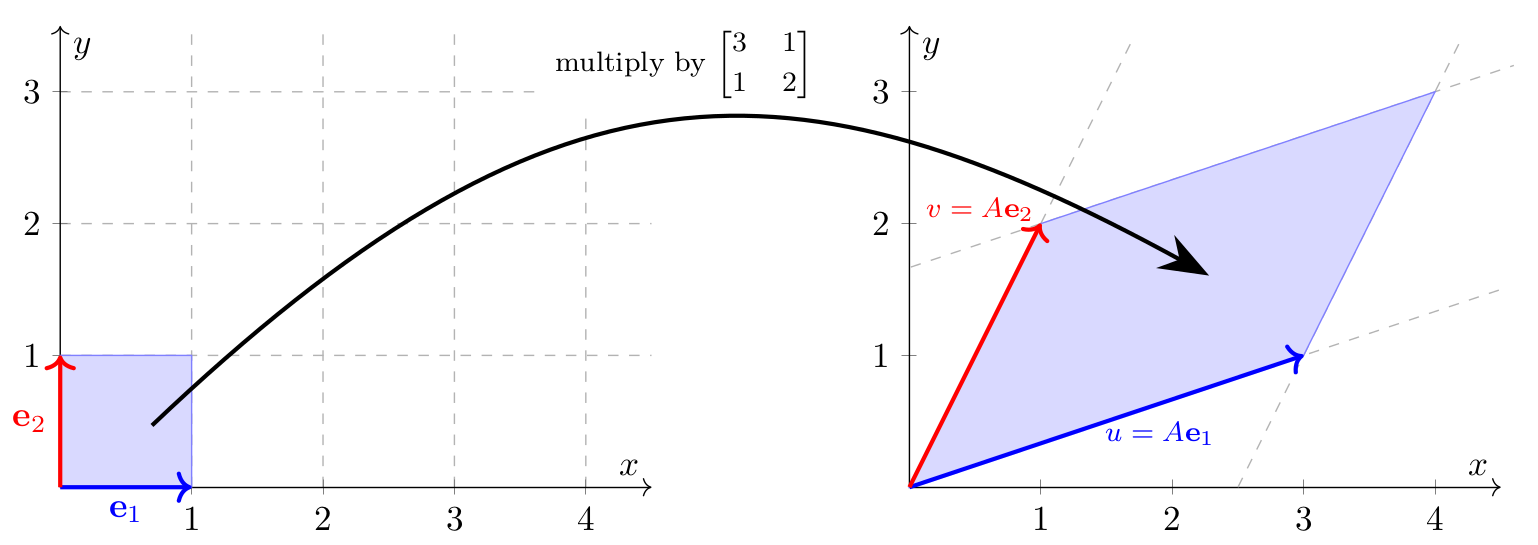
\includegraphics[scale=.3]{images/linear-transform-first-example}
  % \begin{tikzpicture}
  %   % --- Left axis ---
  %   \begin{axis}[
  %     name=left,
  %     at={(0,0)}, anchor=south west,
  %     axis lines=center,
  %     xmin=0, xmax=4.5,
  %     ymin=0, ymax=3.5,
  %     xtick={1,2,3,4},
  %     ytick={1,2,3},
  %     xlabel={$x$}, ylabel={$y$},
  %     axis line style={->},
  %     width=7.5cm, height=6.2cm,
  %     clip=false,
  %     grid=major,
  %     major grid style={dashed,draw=gray!60}
  %     ]
  %     % unit square + unit vectors
  %     \addplot[fill=blue!15, draw=blue!50] coordinates {(0,0) (1,0) (1,1) (0,1)} -- cycle;
  %     \addplot[very thick,->,blue] coordinates {(0,0) (1,0)} node[pos=0.5, below] {$\mathbf e_{1}$};
  %     \addplot[very thick,->,red]  coordinates {(0,0) (0,1)} node[pos=0.5, left] {$\mathbf e_{2}$};
  %   \end{axis}

  %   % --- Right axis ---
  %   \begin{axis}[
  %     name=right,
  %     at={(8.5cm,0)}, anchor=south west, % adjust horizontal gap if desired
  %     axis lines=center,
  %     xmin=0, xmax=4.5,
  %     ymin=0, ymax=3.5,
  %     xtick={1,2,3,4},
  %     ytick={1,2,3},
  %     xlabel={$x$}, ylabel={$y$},
  %     axis line style={->},
  %     width=7.5cm, height=6.2cm,
  %     clip=false
  %     ]
      
  %     % Define u = Ae1 and v = Ae2
  %     \def\ux{3}\def\uy{1}    % u = (3,1)
  %     \def\vx{1}\def\vy{2}    % v = (1,2)

  %     % --- Custom "grid" aligned with u and v ---
  %     % Lines parallel to v, offset by k*u   (images of x = k)
  %     \foreach \k in {0}{
  %       \addplot[thin,gray!60,dashed]
  %       plot[domain=0:1.7, samples=2]
  %       ({\k*\ux + x*\vx},{\k*\uy + x*\vy});
  %     }

  %     \foreach \k in {1}{
  %       \addplot[thin,gray!60,dashed]
  %       plot[domain=-.5:1.2, samples=2]
  %       ({\k*\ux + x*\vx},{\k*\uy + x*\vy});
  %     }

   
  %     % Lines parallel to u, offset by k*v   (images of y = k)
  %     \foreach \k in {0}{
  %       \addplot[thin,gray!60,dashed]
  %       plot[domain=0:1.5, samples=2]
  %       ({\k*\vx + x*\ux},{\k*\vy + x*\uy});
  %     }
  %     \foreach \k in {1}{
  %       \addplot[thin,gray!60,dashed]
  %       plot[domain=-.33:1.2, samples=2]
  %       ({\k*\vx + x*\ux},{\k*\vy + x*\uy});
  %     }

  %     % image of unit square under A: Ae1=(3,1), Ae2=(1,2)
  %     \addplot[fill=blue!15, draw=blue!50] coordinates {(0,0) (3,1) (4,3) (1,2)} -- cycle;
  %     \addplot[very thick,->,blue] coordinates {(0,0) (3,1)}
  %     node[xshift=4pt,pos=0.6, below] {{\footnotesize $u=A\mathbf e_{1}$}};
  %     \addplot[very thick,->,red]  coordinates {(0,0) (1,2)} node[xshift=2pt,yshift=4pt,pos=1, left]  {{\footnotesize$v=A\mathbf e_{2}$}};
  %   \end{axis}

  %   % --- Arching arrow + label between plots ---

  %   \draw[very thick, -{Stealth[length=5mm]}]
  %   ([xshift=-5cm,yshift=-4cm]left.north east)
  %   .. controls ($(left.north east)+(-1,-.2)$) and ($(right.north west)+(-1.2,-.2)$) ..
  %   ([xshift=3cm,yshift=-2.5cm]right.north west)
  %   node[pos=0.5, above=1pt, fill=white, xshift=3pt, yshift=1pt]
  %   {{\footnotesize multiply by $\displaystyle \begin{bmatrix}3&1\\[2pt]1&2\end{bmatrix}$}};
  % \end{tikzpicture}
\end{center}

The effect of applying $A$ is to transform space (i.e., the plane) by
stretching it in some way. For this particular matrix, the unit square get
mapped to the shown parallelogram. Squares adjacent to the unit square get
sent to adjacent parallelograms.

\subsection{The ``volume scaling factor'' of a transformation}
\label{sec:volume-scaling-factor-transformation}
\textbf{Question:} By what factor does the matrix
$\begin{bmatrix}3&1\\1&2\end{bmatrix}$ scale the area of a region in space?


\fl{Answer:} The unit square has area 1. What about the parallelogram?
\begin{center}
  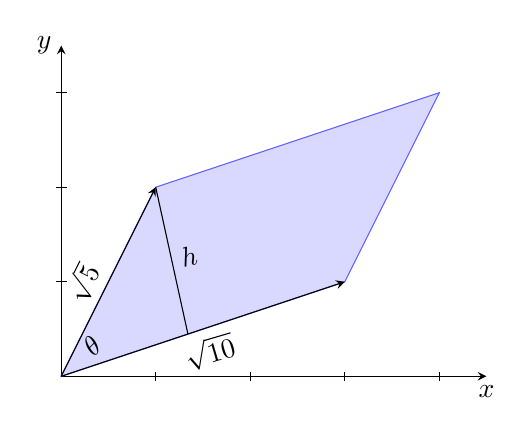
\begin{tikzpicture}[scale=1.2,>=stealth]
    % Axes (positive quadrant)
    \draw[->] (0,0) -- (4.5,0) node[below] {$x$}; \draw[->] (0,0) -- (0,3.5)
    node[left] {$y$};

    % Ticks and labels
    \foreach \x in {1,2,3,4} { \draw (\x,-.05) -- (\x,0.05); } \foreach \y in
    {1,2,3} { \draw (-.06,\y) -- (0.06,\y); }

    % Shade the original unit square

    % Define transformed unit vectors
    \coordinate (a1) at (3,1); \coordinate (a2) at (1,2);

    % Shade parallelogram spanned by a1 and a2
    \fill[blue!15] (0,0) -- (a1) -- ($ (a1)+(a2) $) -- (a2) -- cycle;
    \draw[blue!60] (0,0) -- (a1) -- ($ (a1)+(a2) $) -- (a2) -- cycle;

    % Unit vectors under transformation
    \draw[->] (0,0) -- (a2) node[sloped, rotate=0, pos=.6, above, left,
    xshift=-2pt, yshift=8pt] {$\sqrt{5}$}; \draw[->] (0,0) -- (a1)
    node[sloped, rotate=-2, pos=.5, below] {$\sqrt{10}$};

    % Drop the perpendicular
    \draw[black] (1,2) -- (1.34,.45) node[midway, sloped,
    rotate=90,right]{$h$} ;

    % Label the angle
    \draw[black] (.2,.2) node[sloped, rotate=45, above, right] { $\theta$ };
  \end{tikzpicture}
\end{center}
The parallelogram has area
\begin{equation}\label{eq:parallelogram-area}
  (\text{area of parallelogram}) =  (\text{base})\times(\text{height})
\end{equation}
In this case, the base of the parallelogram is $|u| = \sqrt{10}$. To find the
height $h$, use the definition of $\sin(\theta)$:
\begin{equation*}
  \sin(\theta) = \frac{\text{opposite}}{\text{hypotenuse}} = \frac{h}{\sqrt{5}}.
\end{equation*}
which implies
\begin{equation*}
  h = \sqrt{5} \sin(\theta)
\end{equation*}
We already know that $\cos(\theta) = \frac{1}{\sqrt{2}}$ by
\cref{eq:cosine-example}. Therefore
\begin{align*}
  \sin^{2}(\theta)
  &= 1-\cos^{2}(\theta) &&\text{ (since  }\sin^{2}(\theta)+\cos^{2}(\theta)=1)\\
  &= 1-\frac{1}{2}\\
  &=\frac{1}{2}.
\end{align*}
Taking square roots, we get $\sin(\theta) = \frac{1}{\sqrt{2}}$. Hence
$h = \frac{\sqrt{5}}{\sqrt{2}}.$ Therefore, by \cref{eq:parallelogram-area},
\begin{equation*}
  (\text{area of parallelogram}) = \left( \sqrt{10} \right)  \left( \frac{\sqrt{5}}{\sqrt{2}}  \right) =5.
\end{equation*}
To conclude, the linear transformation of space obtained by multiplying every
vector by the matrix $A=
\begin{bmatrix}
  1&3\\
  2&1
\end{bmatrix}$
took a region of area 1 (the unit square) and mapped it to a parallelogram of
area 5. The scaling is uniform throughout the plane, so every region of area 1
gets mapped to a region of area 5. In other words, the transformation scales
the volume by a factor $5$.


Now let's look at the determinant of the matrix:
\begin{equation*}
  \det \begin{bmatrix}
    3&1\\
    1&2
  \end{bmatrix}
  =3\cdot2 - 1\cdot1 = 5
\end{equation*}
The determinant is also 5. This is not a coincidence. \textbf{The determinant
  tells us how much space gets scaled by the linear transformation induced
  by the matrix.}

\subsection{How do we interpret the determinant when it's zero or negative?}
The determinant measures how much the linear transformation scales volume. But
then what does it mean geometrically for a matrix to have determinant zero or
negative?

\begin{itemize}
  \item If the determinant is zero, that means regions with positive area get
  mapped to regions of zero area. \textbf{This always occurs as a result of
    dimension collapse.} For example, the following matrix has determinant
  zero:
  \begin{equation*}
    \begin{bmatrix}
      1&0\\
      0&0
    \end{bmatrix}
  \end{equation*}
  Note that
  \begin{equation*}
    \begin{bmatrix}
      1&0\\
      0&0
    \end{bmatrix}
    \begin{bmatrix}
      x\\y
    \end{bmatrix}
    =
    \begin{bmatrix}
      x\\0
    \end{bmatrix}
  \end{equation*}
  Geometrically, this matrix projects every point in the plane to its location
  on the $x$-axis. This means that every point in the plane (a 2-dimensional
  surface) gets mapped to the $x$-axis (a 1-dimensional line with zero area).
  The dimension collapse here is the reduction in dimension from 2D to 1D.

  Another example would be a transformation that projects every point in 3D
  space onto a specified plane; this is because mapping a 3D region onto a 2D
  plane destroys volume. An example of such a transformation is obtained from
  the matrix
  \begin{equation*}
    P=
    \begin{bmatrix}
      1&0&0\\
      0&1&0\\
      0&0&0
    \end{bmatrix}
  \end{equation*}
  which projects points in 3D space onto the $xy$-plane. We haven't discussed
  how to define the determinant for $3\times 3$ matrices, but based on our
  geometric intuition, we'd expect $P$ to have determinant zero (it does).
  
  \item If the determinant is negative, that means the transformation reverses
  the orientation of space in the same way a mirror changes left and right
  hands. In 2D, this occurs when the transformation reflects the plane across
  a line. For example, the matrix
  \begin{equation*}
    R =
    \begin{bmatrix}
      0&1\\
      1&0
    \end{bmatrix}
  \end{equation*}
  reflects the $xy$-plane across the line $y=x$, but doesn't stretch space at
  all. The determinant is $-1$. Under this transformation, regions don't
  stretch or shrink, but they do get flipped.

  Another example can be obtained if we decided to \textit{combine} two
  transformations:
  \begin{itemize}
    \item \textbf{First}, flip the $xy$-plane using $R$.
    \item \textbf{Then}, transform space using the matrix $A$.
  \end{itemize}
  To combine these two tranformations, we multiply the matrices like this:
  \begin{equation*}
    AR =
    \underbrace{\begin{bmatrix}
      3&1\\
      1&2
    \end{bmatrix}}_{\tiny 2^{\rm nd}}
    \underbrace{\begin{bmatrix}
        0&1\\
        1&0
      \end{bmatrix}}_{\tiny 1^{\rm st}}
    =
    \begin{bmatrix}
      3&1\\
      1&2
    \end{bmatrix}
  \end{equation*}

  This new matrix has determinant $-5$. It is similar to the matrix $A$ we
  considered earlier, but the columns are swapped. Geometrically, this matrix
  transforms space by first reflecting the plane across the line $y=x$ and
  then doing the same stretchy thing done by the previous matrix.

  The picture is almost the same as the previous one, but note how the red and
  blue vectors swapped compared to the first picture. The orientation has
  changed, which is why the determinant is negative.
\end{itemize}

\begin{center}
  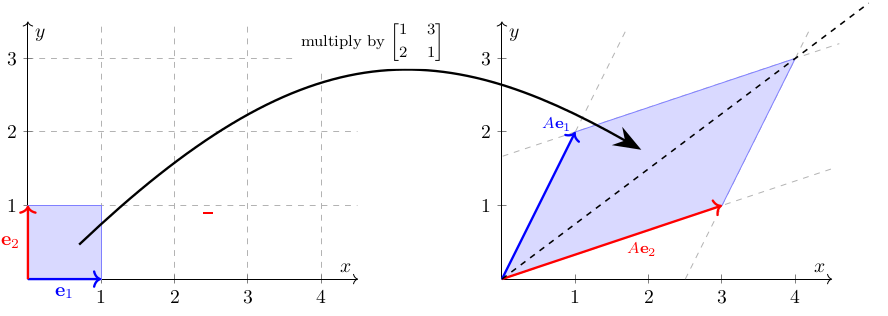
\includegraphics[scale=.4]{linear-transformation-first-exampled-flipped.png}
\end{center}
% \begin{center}
%   \begin{tikzpicture}
%     %   --- Left axis ---
%     \begin{axis}[
%       name=left,
%       at={(0,0)}, anchor=south west,
%       axis lines=center,
%       xmin=0, xmax=4.5,
%       ymin=0, ymax=3.5,
%       xtick={1,2,3,4},
%       ytick={1,2,3},
%       xlabel={$x$}, ylabel={$y$},
%       axis line style={->},
%       width=7.5cm, height=6.2cm,
%       clip=false,
%       grid=major,
%       major grid style={dashed,draw=gray!60}
%       ]
%       %     unit square + unit vectors
%       \addplot[fill=blue!15, draw=blue!50] coordinates {(0,0) (1,0) (1,1) (0,1)} -- cycle;
%       \addplot[very thick,->,blue] coordinates {(0,0) (1,0)} node[pos=0.5, below] {$\mathbf e_{1}$};
%       \addplot[very thick,->,red]  coordinates {(0,0) (0,1)} node[pos=0.5, left] {$\mathbf e_{2}$};
%     \end{axis}

%     %   --- Right axis ---
%     \begin{axis}[
%       name=right,
%       at={(8.5cm,0)}, anchor=south west, % adjust horizontal gap if desired
%       axis lines=center,
%       xmin=0, xmax=4.5,
%       ymin=0, ymax=3.5,
%       xtick={1,2,3,4},
%       ytick={1,2,3},
%       xlabel={$x$}, ylabel={$y$},
%       axis line style={->},
%       width=7.5cm, height=6.2cm,
%       clip=false
%       ]
  
%       %     Define u = Ae1 and v = Ae2
%       \def\ux{3}\def\uy{1}    % u = (3,1)
%       \def\vx{1}\def\vy{2}    % v = (1,2)

%       %     --- Custom "grid" aligned with u and v ---
%       %     Lines parallel to v, offset by k*u   (images of x = k)
%       \foreach \k in {0}{
%       \addplot[thin,gray!60,dashed]
%       plot[domain=0:1.7, samples=2]
%       ({\k*\ux + x*\vx},{\k*\uy + x*\vy});
%     }

%       \foreach \k in {1}{
%       \addplot[thin,gray!60,dashed]
%       plot[domain=-.5:1.2, samples=2]
%       ({\k*\ux + x*\vx},{\k*\uy + x*\vy});
%     }

  
%       %     Lines parallel to u, offset by k*v   (images of y = k)
%       \foreach \k in {0}{
%       \addplot[thin,gray!60,dashed]
%       plot[domain=0:1.5, samples=2]
%       ({\k*\vx + x*\ux},{\k*\vy + x*\uy});
%     }
%       \foreach \k in {1}{
%       \addplot[thin,gray!60,dashed]
%       plot[domain=-.33:1.2, samples=2]
%       ({\k*\vx + x*\ux},{\k*\vy + x*\uy});
%     }

    
%       %     image of unit square under A: Ae1=(3,1), Ae2=(1,2)
%       \addplot[fill=blue!15, draw=blue!50] coordinates {(0,0) (3,1) (4,3) (1,2)} -- cycle;
%       \addplot[very thick,->,red] coordinates {(0,0) (3,1)}
%       node[xshift=4pt,pos=0.6, below] {{\footnotesize $A\mathbf e_{2}$}};
%       \addplot[very thick,->,blue]  coordinates {(0,0) (1,2)} node[xshift=2pt,yshift=4pt,pos=1, left]  {{\footnotesize$A\mathbf e_{1}$}};


%       % axis of refletion
%       \addplot[black, thick, dashed, domain=0:5] {.75*x};
      
%     \end{axis}

    
%     %   --- Arching arrow + label between plots ---

%     \draw[very thick, -{Stealth[length=5mm]}]
%     ([xshift=-5cm,yshift=-4cm]left.north east)
%     .. controls ($(left.north east)+(-1,-.2)$) and ($(right.north west)+(-1.2,-.2)$) ..
%     ([xshift=2.5cm,yshift=-2.3cm]right.north west)
%     node[pos=0.5, above=1pt, fill=white, xshift=3pt, yshift=1pt]
%     {{\footnotesize multiply by $\displaystyle \begin{bmatrix}1&3\\[2pt]2&1\end{bmatrix}$}};
%   \end{tikzpicture}
% \end{center}

\newpage
\section{2025-09-12 | Week 03 | Lecture 08}
\textit{This lecture is based on sections 1.3 in your textbook}



\begin{center}
  \begin{tcolorbox}[width=0.9\textwidth, colback=white, colframe=black]
    \textit{\textbf{The nexus question of this lecture:} What are the key
      properties of the matrix inverse?}
  \end{tcolorbox}
\end{center}




\subsection{What is a matrix inverse?}
\begin{definition}[Matrix Inverse]
  \label{def:matrix-inverse}  
  The matrix $A$ is \demph{invertible} if there is a matrix $A^{-1}$ such that
  \begin{equation*}
    A^{-1}A = I \quad \text{and} \quad AA^{-1}=I
  \end{equation*}
  If so we call $A^{-1}$ the \demph{inverse} of $A$.
\end{definition}

\fl{Note:}
\begin{itemize}
  \item Invertible matrices are always square. Nonsquare matrices are not
  invertible.
  
  \item Whatever $A$ does, $A^{-1}$ undoes. If $A$ stretches spaces, $A^{-1}$
  compresses it back. If $A$ flips space, $A^{-1}$ flips it back. If $A$
  rotates spaces, $A^{-1}$ rotates it back, etc.
\end{itemize}


\begin{theorem}[The socks and shoes property]
  \label{thm:socks-and-shoes-property}
  If $A$ and $B$ are invertible then so is $AB$, and
  \begin{equation*}
    (AB)^{-1} = B^{-1}A^{-1}
  \end{equation*}
\end{theorem}

If you put on socks and then shoes, what is the inverse of that? Take off the
shoes, and then the socks.

Note that \cref{thm:socks-and-shoes-property} has two conclusions: first, that
products of matrices are invertible, and second the formula
$(AB)^{-1}=B^{-1}A^{-1}$.

\begin{proof}[Proof of \cref{thm:socks-and-shoes-property}]
  It is sufficient to show that $B^{-1}A^{-1}$ is the inverse of $AB$, which
  we can do by direct computation:
  \begin{equation*}
    (AB)(B^{-1}A^{-1}) = A(BB^{-1})A^{-1} = A(I)A^{-1} = AA^{-1} = I.
  \end{equation*}
  and
  \begin{equation*}
    (B^{-1}A^{-1})(AB) = B^{-1}(A^{-1}A)B = B^{-1}B = I
  \end{equation*}
\end{proof}


\begin{theorem}
  \label{thm:one-sided-inverse-is-enough}
  Suppose that $A$ and $B$ are square matrices such that either $AB=I$ or
  $BA=I$. Then $A$ is an invertible matrix and $A^{-1}=B$
\end{theorem}

I'm going to omit the proof of this theorem, but I will introduce the general
framework that that is used to prove it and results like it, because it is
based on an important idea.

\subsection{Row reduction is multiplication by elementary matrices}
\label{sec:row-reduction-multiplication-elementary-matrices}
Section 1.3 in the textbook provides a framework, based on row reduction, for
deducing properties of inverses. Recall that in row reduction, you have three
basic operations:
\begin{itemize}
  \item swapping two rows
  \item multiplying a row by a number
  \item adding a multiple of a row to another row.
\end{itemize}
These operations can all be done using matrix multiplication, using matrices
called \demph{elementary matrices}. Here are some examples:
\begin{align*}
  \begin{bmatrix}
    0&1\\
    1&0
  \end{bmatrix}
  \begin{bmatrix}
    a&b\\
    c&d
  \end{bmatrix}
  =
  \begin{bmatrix}
    c&d\\
    a&b
  \end{bmatrix}
  &&\text{ $R_{1}\leftrightarrow R_{2} $ }
\end{align*}

\begin{align*}
  \begin{bmatrix}
    5&0\\
    0&1
  \end{bmatrix}
  \begin{bmatrix}
    a&b\\
    c&d
  \end{bmatrix}
  =
  \begin{bmatrix}
    5a&5b\\
    c&d
  \end{bmatrix}
  &&\text{ $5R_{1} \to R_{1}$ }
\end{align*}

\begin{align*}
  \begin{bmatrix}
    1&0\\
    3&1
  \end{bmatrix}
  \begin{bmatrix}
    a&b\\
    c&d
  \end{bmatrix}
  =
  \begin{bmatrix}
    c&d\\
    3a+c&3b+d
  \end{bmatrix}
  &&\text{ $3R_{1}+R_{2}\to R_{2}$ }
\end{align*}

\Fl{Fact:} Elementary matrices are always invertible, because one can always
undo a row operation. Moreover, by \cref{thm:socks-and-shoes-property} (which
tells us that products of invertible matrices are invertible), we also know
that products of elementary matrices are also invertible.

\Fl{What does it all mean?} If you can row reduce a matrix $A$ to $I$, that
means there exists some sequence of elementary matrices $E_{1},\ldots,E_{m}$
such that
\begin{equation*}
  E_{1}E_{2}E_{3}\cdots E_{m}A=I.
\end{equation*}
Letting $M= E_{1}E_{2}E_{3}\cdots E_{m}$, we have
\begin{equation*}
  MA=I.
\end{equation*}
By \cref{thm:one-sided-inverse-is-enough}, this is enough to conclude that $A$
is invertible and 
\begin{equation*}
  A^{-1} = M.
\end{equation*}

We've just proven part of the following theorem:

\begin{theorem}
  Let $A$ be a square matrix. The following are equivalent:
  \begin{enumerate}[label=(\roman*.)]
    \item $A$ can be row-reduced to the identity matrix $I$.
    \item $A$ is invertible.
  \end{enumerate}
\end{theorem}

In particular, we've shown that $(i.)$ implies $(ii.)$. The reverse direction
(that $(ii.)$ implies $(i.)$) can also be proved using this framework of
elementary matrices, but I'd rather spend the time showing an example of how
to compute the inverse of a matrix using row reduction.

\subsection{Computing matrix inverses using row-reduction}
The next example will illustrate a general approach for computing a matrix
inverse.

\begin{example}[Computing the inverse of a matrix]
  \label{ex:computing-inverse-matrix}
  In the previous lecture, we considered the matrix
  \begin{equation*}
    A=
    \begin{bmatrix}
      3&1\\
      1&2
    \end{bmatrix}
  \end{equation*}
  which stretches space in some way, scaling area by a factor of $5$. Suppose
  we wish to find $A^{-1}$.

  Let
  \begin{equation*}
    X =
    \begin{bmatrix}
      x_{11}&x_{12}\\
      x_{21}&x_{22}\\
    \end{bmatrix}
  \end{equation*}
  We need $X$ to satisfy
  \begin{equation*}
    AX =
    \begin{bmatrix}
      1&0\\
      0&1
    \end{bmatrix}
  \end{equation*}
  Writing out $AX$, we have
  \begin{equation*}
    AX =
    \begin{bmatrix}
      3&1\\1&2
    \end{bmatrix}
    \begin{bmatrix}
      x_{11}&x_{12}\\x_{21}&x_{22}
    \end{bmatrix}
    =
    \begin{bmatrix}
      3x_{11}+x_{21}& 3x_{12}+x_{22}\\
      x_{11}+2x_{21}& x_{12}+2x_{22}
    \end{bmatrix}
    \overset{\text{set}}{=}
    \begin{bmatrix}
      1&0\\
      0&1
    \end{bmatrix}
  \end{equation*}
  By setting $AX$ equal to $I$, we have a system of four linear equations in
  four variables $x_{11},x_{12},x_{21},x_{22}$.

  We have a nice way to solve linear systes: row reduction. Moreover, for
  finding inverses, there is a clever way to do it, as I now show.

  \fl{Step 1.} Set up an augmented matrix of the following form:
  \begin{equation*}
    \begin{augmentedmatrix}{cc|cc}
      3&1&1&0\\
      1&2&0&1
    \end{augmentedmatrix}
  \end{equation*}
  \fl{Step 2.} Completely row reduce the matrix until the left part is the
  identity matrix. (I'm skipping these steps). After doing this for this
  example, we get:
  \begin{equation*}
    \begin{augmentedmatrix}{cc|cc}
      1&0&2/5&-1/5\\
      0&1&-1/5&3/5
    \end{augmentedmatrix}
  \end{equation*}
  \fl{Step 3.} Draw the conclusion that $A^{-1}$ is the the matrix to the
  right of the bar:
  \begin{equation*}
    A^{-1} =
    \begin{bmatrix}
      2/5&-1/5\\
      -1/5&3/5
    \end{bmatrix}
  \end{equation*}
\end{example}

\begin{remark}
  The approach in \cref{ex:computing-inverse-matrix} works for larger matrices
  as well, see Example 1 in Section 1.3 of the textbook (p.31).
\end{remark}

\begin{remark}
  Recall that from the previous lecture, we saw that the matrix
  $A=
  \begin{bmatrix}
    3&1\\
    1&2
  \end{bmatrix}
  $ corresponds to a transformation of space that somehow stretched space in a
  way that scaled area by a factor of $5$, because $\det(A)=5$ (see
  \cref{sec:volume-scaling-factor-transformation}). Since $A^{-1}$ undoes
  whatever $A$ did, so it must shrink space by a factor of $5$. Indeed,
  \begin{equation*}
    \det(A^{-1}) 
    = \left(\frac{2}{5}\right)\left(\frac{3}{5}\right)-\left(-\frac{1}{5}\right)\left(-\frac{1}{5}\right) 
    = \frac{6}{25}- \frac{1}{25} 
    = \frac{1}{5}.
  \end{equation*}
\end{remark}


This illustrates the following theorem:
\begin{theorem}
  If $A^{-1}$ exists then
  \begin{equation*}
    \det(A^{-1}) = \frac{1}{\det(A)}.
  \end{equation*}
\end{theorem}
Now that we know the determinant of a matrix measures how space is scaled by
the transformation, the geometric reason why this theorem is true is obvious:
the matrix $A$ transforms space in some way, and then $A^{-1}$ undoes that
transformation. So we are left with the \demph{identity transformation}, which
doesn't change space at all. So if $A$ scales space by a factor of $a$ then
$A^{-1}$ must scale it by a factor of $\frac{1}{a}$. We'll probably give an
actual proof later, but that's the idea.


% \begin{example}[Example 1 in section 1.3]
%   Find the inverse of the matrix
%   \begin{equation*}
%     A= \begin{bmatrix}
%       2&1&3\\
%       2&1&1\\
%       4&5&1
%     \end{bmatrix}
%   \end{equation*}
%   We set up the augmented matrix
%   \begin{equation*}
%     \begin{augmentedmatrix}{ccc|ccc}
%       2&1&3&1&0&0\\
%       2&1&1&0&1&0\\
%       4&5&1&0&0&1
%     \end{augmentedmatrix}.
%   \end{equation*}
%   After row reduction, we obtain
%   \begin{equation*}
%     \begin{augmentedmatrix}{ccc|ccc}
%       1&0&0&-1/3&7/6&-1/6\\
%       0&1&0&1/6&-5/6&1/3\\
%       0&0&1&1/2&-1/2&0
%     \end{augmentedmatrix}.
%   \end{equation*}
%   Then the inverse of $A$ is given by
%   \begin{equation*}
%     A^{-1} =
%     \begin{bmatrix}
%       -1/3&7/6&-1/6\\
%       1/6&-5/6&1/3\\
%       1/2&-1/2&0
%     \end{bmatrix}.
%   \end{equation*}
% \end{example}


\newpage
\section{2025-09-15 | Week 04 | Lecture 09}

\textit{This lecture is based on sections 1.5 and 1.6 in the textbook. We are
  going to skip section 1.7}



\begin{center}
  \begin{tcolorbox}[width=0.9\textwidth, colback=white, colframe=black]
    \textit{\textbf{The nexus question of this lecture:} How do we understand
      (and compute) the determinant, algebraically?}
  \end{tcolorbox}
\end{center}

\subsection{Review of the ``key theorem'' of linear algebra}


\begin{theorem}[The Key Theorem of Linear Algebra (partial version)]
  \label{thm:key-theorem-linear-algebra-(partial-version))}
  Let $A$ be an $n\times n$ matrix. Then the following are equivalent:
  \begin{enumerate}[label=(\roman*.)]
    \item $A^{-1}$ exists (i.e., $A$ is invertible)
    \item $\det A \neq 0$
    \item The linear system $AX=B$ has a unique solution for each $B\in
    \R^{n}$.
    \item $A$ is row equivalent to $I$
    \item ... 
  \end{enumerate}
\end{theorem}

Property (iv.) says we can row reduce $A$ into $I$. The term for this is ``row
equivalence''. Precisely, If $A$ and $B$ are matrices, we say that $A$ is
\demph{row equivalent} to $B$ if there is a sequence of elementary row
operations which if applied to $A$ will result in $B$.


\subsection{Definition of the determinant}

Consider a square matrix
\begin{equation*}
  A =
  \begin{bmatrix}
    a_{11}&a_{12}&\ldots& a_{1n}\\
    a_{21}&a_{22}&\ldots& a_{2n}\\
    \vdots&\vdots & &\vdots \\
    a_{n1}&a_{n2}&\ldots& a_{nn}
  \end{bmatrix}.
\end{equation*}
Given an entry $a_{ij}$, the \demph{minor} of $a_{ij}$, denoted $M_{ij}$, is the matrix
obtained from $A$ by deleting row $i$ and column $j$ of $A$. For example, if
\begin{equation*}
  A =
  \begin{bmatrix}
    a_{11},a_{12},a_{13}\\
    a_{21},a_{22},a_{23}\\
    a_{31},a_{32},a_{33}\\
  \end{bmatrix}
\end{equation*}
then some minors are
\begin{equation*}
  M_{11} =
  \begin{bmatrix}
    a_{12}&a_{13}\\
    a_{22}&a_{23}
  \end{bmatrix},
  \quad
  M_{12} =
  \begin{bmatrix}
    a_{21}&a_{23}\\
    a_{31}&a_{33}
  \end{bmatrix},
  \quad \text{and} \quad
  M_{32} =
  \begin{bmatrix}
    a_{11}&a_{13}\\
    a_{21}&a_{23}
  \end{bmatrix}.
\end{equation*}

\begin{definition}[Determinant]
  \label{def:determinant}
  For a $1\times 1$ matrix, $A=[a_{11}]$, we define $\det(A) =1$. If $A$ is an
  $n\times n$ matrix with $n \geq 2$, we define the determinant recursively as
  \begin{equation}\label{eq:determinant-definition}
    \det(A) = \sum_{j=1}^{n}(-1)^{j+1}a_{1j}\det(M_{1j}).
  \end{equation}
\end{definition}
\Fl{Note:} Note that the determinant is defined only for square matrices.

Geometrically, the determinant is the (signed) volume scaling factor of the
transformation of space, which is very useful to keep in mind.
\cref{def:determinant} is also useful because it allows us to see how to
actually compute determinants.

For a $2\times 2$ matrix, \cref{def:determinant} simplifies to
\begin{equation*}
  \det \left(
    \begin{bmatrix}
      a_{11}&a_{12}\\
      a_{21}&a_{22}
    \end{bmatrix}
  \right) = a_{11}a_{22}-a_{12}a_{21}.
\end{equation*}

To simplify notation, we use vertical bars to denote determinant
$|A|:=\det(A)$, or something like this:
\begin{equation*}
  \begin{vmatrix}
    a_{11}&a_{12}\\
    a_{21}&a_{22}
  \end{vmatrix}
  :=
  \det \left(
    \begin{bmatrix}
      a_{11}&a_{12}\\
      a_{21}&a_{22}
    \end{bmatrix}
    \right).
\end{equation*}

\begin{example}[Computing the determinant of a $3\times 3$ matrix]
  \label{ex:computing-determinant-3times-3-matrix}
  \begin{align*}
    \begin{vmatrix}
      2&3&-2\\
      -1&6&3\\
      4&-2&1
    \end{vmatrix}
        &=
          2
          \begin{vmatrix}
            6&3\\
            -2&1
          \end{vmatrix}
                -3
                \begin{vmatrix}
                  -1&3\\
                  4&1
                \end{vmatrix}
                     +(-2)
                     \begin{vmatrix}
                       -1&6\\
                       4&-2
                     \end{vmatrix}\\
       &=2 \left[ 6\cdot1 - 3(-2) \right]
         -3 \left[ (-1)1 - 3\cdot4 \right]
         -2 \left[ (-1)(-2)-6\cdot4 \right]\\ 
       &=107.
  \end{align*}
\end{example}

\subsection{Computing determinants using cofactor expansions}
The formula for the determinant in \cref{def:determinant} is called a
\demph{cofactor expansion} (there are other formulas). A \demph{cofactor} of
an entry $a_{ij}$ is the quantity
\begin{equation*}
  C_{ij} = (-1)^{i+j}\det(M_{ij})
\end{equation*}
so our formula in \cref{eq:determinant-definition} can be written as
\begin{equation*}
  \det(A) = \sum_{j=1}^{n}  a_{1j}C_{1j}. 
\end{equation*}
This is called the \demph{cofactor expansion about the first row.} The next
theorem tell us that, in fact, we could have picked \textit{any} row or column
and done a similar calculation to get the determinant:
\begin{theorem}[Cofactor Expansion]
  \label{thm:cofactor-expansion}
  If $A$ is an $n\times n$ matrix with $n \geq 2$, then
  \begin{enumerate}[label=(\roman*.)]
    \item For any fixed $i=1,2,\ldots,n,$ we have
    \begin{equation*}
      \det(A) = \sum_{j=1}^{n}a_{ij}C_{ij} \quad \text{(cofactor expansion
        about the $i^{\rm th}$ row)}
    \end{equation*}
    \item For any fixed $j=1,2,\ldots,n$, we have
    \begin{equation*}
      \det(A) = \sum_{i=1}^{n}a_{ij}C_{ij} \quad \text{(cofactor expansion
        about the $j^{\rm th}$ column)} 
    \end{equation*}
  \end{enumerate}
\end{theorem}
This theorem is proved by induction on $n$ in section 1.7, but the proof is
technical, so we'll skip it. Two examples will illustrate this theorem.

\begin{example}[Alternative cofactor expansions]

  Let's compute the determinant of the matrix from
  \cref{ex:computing-determinant-3times-3-matrix} in two different ways, using
  \cref{thm:cofactor-expansion}:
  
 The cofactor expansion about the third row:
  \begin{align*}
    \begin{vmatrix}
      2&3&-2\\
      -1&6&3\\
      4&-2&1
    \end{vmatrix}
        &=
          a_{31}C_{31}+a_{32}C_{32}+a_{33}C_{33}\\
       &= 4
          \begin{vmatrix}
            3&-2\\
            6&3
          \end{vmatrix}
                -(-2)
                \begin{vmatrix}
                  2&-2\\
                  -1&3
                \end{vmatrix}
                     +1
                     \begin{vmatrix}
                       2&3\\
                       -1&6
                     \end{vmatrix}\\
       &=107.
  \end{align*}
  The cofactor expansion about the second column:
  \begin{align*}
    \begin{vmatrix}
      2&3&-2\\
      -1&6&3\\
      4&-2&1
    \end{vmatrix}
       &= a_{21}C_{21}+a_{22}C_{22}+a_{32}C_{32}\\
       &= -3
          \begin{vmatrix}
            -1&3\\
            4&1
          \end{vmatrix}
               +6
               \begin{vmatrix}
                 2&-2\\
                 4&1
               \end{vmatrix}
                     -(-2)
                     \begin{vmatrix}
                       2&-2\\
                       -1&3
                     \end{vmatrix}\\
       &=107.
  \end{align*}
  The $-3$ at the beginning of this is not a typo. It's $-3$ rather than $3$
  because of the $-1$ introduced by the cofactor $C_{21}$, which is
  $C_{21}=(-1)^{2+1} \begin{vmatrix}
                       -1&3\\
                       4&1
                     \end{vmatrix} = - \begin{vmatrix}
                                          -1&3\\
                                          4&1
                                        \end{vmatrix}.$
\end{example}

\subsection{Key properties of the determinant}

\begin{theorem}
  
  If $I$ is an $n\times n$ identity matrix, then $\det(I)=1$. If $\mathbf{O}$
  is an $n\times n$ zero matrix, then $\det(\mathbf{O})=0$.
\end{theorem}

I claim that when this theorem is considered geometrically, its truth becomes
obvious. Why is it obvious?

\begin{itemize}
  \item Because the identity matrix $I$ corresponds to the
  transformation of space that \textit{doesn't change anything}. This is called
  the \demph{identity transformation}. This doesn't stretch (or reflect) space
  at all, and hence areas/volumes are not changed at all. So the determinant,
  being the volume scaling factor of the transformation, is $1$.
  \item And because the zero matrix $\mathbf{O}$ maps every vector to the
  vector $\vec{0}=(0,0,\ldots,0)$. This means $\mathbf{O}$ collapses the
  entirety of $n$-dimensional space into a single point (i.e., the origin),
  which has dimension zero. The dimensional collapse means that area/volume
  gets destroyed, and hence $\det(\mathbf{O})=0$.
\end{itemize}


The next theorem says that the determinant ``preserves multiplication''.

\begin{theorem}[The determinant preserves multiplication]
  If $A$ and $B$ are $n\times n$ matrices, then
  \begin{equation*}
    \det(AB) = \det(A)\det(B).
  \end{equation*}
\end{theorem}



The textbook provides a nice algebraic proof of this in terms of the row
reduciton framework presented in
\cref{sec:row-reduction-multiplication-elementary-matrices} [namely, the proof
of Theorem 1.24 in section 1.6 (p.52-53), which I encourage you to read]. But
I claim that this theorem is \textit{obvious} when its geometric meaning is
considered (i.e., in terms of matrices as transformations of space). We'll
start with this idea next lecture.

\newpage
\section{2025-09-17 | Week 04 | Lecture 10}
\textit{This lecture is based on sections 1.5 and 1.6 in the textbook.}
\begin{center}
  \begin{tcolorbox}[width=0.9\textwidth, colback=white, colframe=black]
    \textit{\textbf{The nexus question of this lecture:} What are some useful
      connections between the geometric and algebraic interpretations of the
      the determinant?}
  \end{tcolorbox}
\end{center}

Recall that for $A\in M_{n\times n}$, we have
\begin{equation*}
  \det(A) 
  = \left( \overset{\text{the (signed) volume scaling }}{{\scriptsize \text{factor of the transformation}}} \right) 
  = \sum_{j=1}^{n} a_{1j}(-1)^{1+j}\det(M_{1j}) 
\end{equation*}
These are the geometric interpretation (left) and algebraic interpretation
(right) of the determinant. 

\subsection{Determinants preserve multiplication}


\begin{theorem}[The determinant preserves multiplication]
  \label{thm:determinant-preserves-multiplication}
  If $A$ and $B$ are $n\times n$ matrices, then
  \begin{equation*}
    \det(AB) = \det(A)\det(B).
  \end{equation*}
\end{theorem}
\Fl{Key background - Matrices as tranformations:}
The geometric idea of understanding matrices as transformations of space makes
this theorem obvious. Let $P=AB$. The transformation of space given by $P$ is
\begin{itemize}
  \item first, do the transformation of $B$
  \item then, do the transformation of $A$.
\end{itemize}

Why is it in this order? To see why, let $P=AB$, and consider how $P$ acts on
a vector $X$:
\begin{equation*}
  PX = (AB)X = A(BX)
\end{equation*}
The placement of the parentheses means we first transform $X$ with $B$. Then,
whatever we get from that, we transform with $A$. In other words, the product
$P$ acts on $X$ by first applying $B$ and then applying $A$.

In other words, matrix multiplication can be understood as \textit{function
  composition} of the transformations of $A$ and $B$. 

\Fl{Explanation of why \cref{thm:determinant-preserves-multiplication} is
  true:} When two transformations are composed (by multiplying the matrices),
the total scaling is the product of the scalings of each transformation. If
$B$ scales volume by a factor of $2$, and $A$ scales it again by a factor of
$5$, then the final scaling induced by $P=AB$ will be $10$. In symbols
\begin{equation*}
  \det(AB) = 10 = 5\cdot 2 = \det(A)\det(B).
\end{equation*}
The idea is similar when the negative determinants (i.e., corresponding to
transformations which include some sort of reflection) are used.

One consequence of \cref{thm:determinant-preserves-multiplication} is the
following relationship:
\begin{theorem}
  If $A$ is invertible, then
  \begin{equation*}
    \det(A^{-1})=\frac{1}{\det(A)}
  \end{equation*}
\end{theorem}
\begin{proof}
  \begin{align*}
    \det(A)\det(A^{-1}) 
    &= \det(AA^{-1}) &&\text{(by \cref{thm:determinant-preserves-multiplication})}\\
    &= \det(I) &&\text{(since $AA^{-1}=I$)}\\ 
    &=1 &&\text{(since the determinant of the identity matrix is always 1).}
  \end{align*}
  Dividing both sides by $\det(A^{-1})$ gives the result.
\end{proof}


\subsection{Determinants and dimension collapse}
The next theorem describes a class of matrices which have dimension zero
because they collapse space:

\begin{theorem}[Zero row/column]
  \label{thm:zero-rowcolumn}
  Let $A$ be an $n\times n$ matrix. If $A$ has a row of zeros (or a column of
  zeroes), then the determinant is zero.
\end{theorem}


\begin{proof}
  Suppose that the $k^{\rm th}$ row of $A$ has only zero entries. That means
  \begin{equation*}
    a_{k1}=0,\quad a_{k2}=0, \quad a_{k3}=0,\quad\ldots \quad \text{and} \quad a_{kn}=0
  \end{equation*}
  By \cref{thm:cofactor-expansion}(i.),
  \begin{equation*}
    \det(A) = \sum_{j=1}^{n}a_{ij}C_{ij} 
  \end{equation*}
  for any choice of $j\in \left\{1,2,\ldots,n\right\}$. Picking $i=k$, we get
  \begin{align*}
    \det(A) 
    &= \sum_{j=1}^{n}a_{kj}C_{kj}\\
    &= \sum_{j=1}^{n}(0)C_{kj}\\
    &=0.
  \end{align*}
  The proof for the case where $A$ has a column of zero entries is similar.
\end{proof}

To see why \cref{thm:zero-rowcolumn} is true geometrically, it suffices to
consider an example
\begin{example}[A row of zeroes implies zero determinant]
  \label{ex:row-zeroes-implies-zero-determinant}
  \begin{equation*}
    A =
    \begin{bmatrix}
      4&5&-1\\
      6&2&3\\
      0&0&0\\
    \end{bmatrix}
  \end{equation*}
  \begin{equation*}
    \begin{bmatrix}
      4&5&-1\\
      6&2&3\\
      0&0&0\\
    \end{bmatrix}
    \begin{bmatrix}
      x\\y\\z
    \end{bmatrix}
    =
    \begin{bmatrix}
      4x+5y-z\\ 6x+2y+3z \\0
    \end{bmatrix}
  \end{equation*}
  As a transformation of space, this matrix sends every point $
  \begin{bmatrix}
    x\\y\\z
  \end{bmatrix}
  $ to another point of the form $
  \begin{bmatrix}
    *\\ * \\ 0
  \end{bmatrix}
  $. Therefore every point gets mapped to a point in the set
  \begin{equation*}
    \left\{(x,y,z)\in \R^{3}: z=0\right\} 
  \end{equation*}
  This is the plane $z=0$. So the matrix $A$ effectuates a dimension collapse,
  from 3 dimensonal space into to a 2-dimensional plane. This destroys volume,
  so $\det(A)=0$.
\end{example}

\begin{example}[Remark on \cref{thm:zero-rowcolumn}]
  Of course, not every matrix that has determinant zero has a row or column of
  zeroes. For example, one can check that
  \begin{equation*}
    \begin{vmatrix}
      0&1&2\\
      3&1&2\\
      5&2&4
    \end{vmatrix}=0.
  \end{equation*}
  Yet this matrix doesn't have a row or column of zeroes. Notice that the
  second and third columns are colinear: one is a scalar multiple of the
  other. This has something to do with it. 
\end{example}

\subsection{Determinants and axis-aligned stretching}
A special case of matrices are those which \demph{triangular}. A matrix is
said to be \demph{upper triangular}, if all entries below the main diagonal
are equal to zero. Like this:
\begin{equation*}
  \begin{bmatrix}
    1&2&3\\
    0&4&5\\
    0&0&6 
  \end{bmatrix}
  \quad \text{or} \quad
  \begin{bmatrix}
    1&2&3&4\\
    0&5&6&7\\
    0&0&8&9\\
    0&0&0&10\\
  \end{bmatrix}
\end{equation*}
Similarly, a matrix is said to be \demph{lower triangular} if all the entries
above the main diagonal are zero.

Triangular matrices always correspond to some combination of the following two
transformations:
\begin{itemize}
  \item stretch space in the direction of one or more the coordinate axes
  (e.g., in the direction of the $x$-axis or $y$-axis or $z$-axis, etc.)
  \item possibly also one or more ``shear transforms''
\end{itemize}
Shear transformations don't stretch space at all, so the determinant of a
triangular matrix is determined only by how much it stretches space in the
directions of the coordinate axes $x$, $y$, and $z$ directions. And it turns
out, these stretchings are easy to see just by looking at the matrix.

Here's an example. The matrix
\begin{equation*}
  A=\begin{bmatrix}
    1&2&3\\
    0&4&5\\
    0&0&6 
  \end{bmatrix}
\end{equation*}
stretches space in the $x$ direction by $1$, stretches spaces in the $y$
direction by $4$, and stretches space in the $z$ direction by $6$. The overall
stretching of volume is therefore $24=1\cdot4\cdot6$. So
\begin{equation*}
  \det(A) = 1\cdot4\cdot6=24.
\end{equation*}


This is the idea behind the following theorem:

\begin{theorem}[Determinants of triangular matrices]
  \label{thm:determinants-triangular-matrices}
  Let $T=(t_{ij})\in M_{n\times n}(\R)$ be a triangular matrix . Then
  \begin{equation*}
    \det(T) = t_{11}t_{22}\cdots t_{nn}.
  \end{equation*}
  In words, the determinant equals the product of the diagonal entries.
\end{theorem}

This theorem can be proved by induction on $n$.
% \begin{proof}
%   We will prove the case where $T$ is lower triangular. The case where $T$ is
%   upper triangular can be proved similarly. (homework?)
  
%   The proof is by induction on $n$.

%   \Fl{Case 1. Suppose $n=2$. (``base case'').}

%   Let
%   \begin{equation*}
%     T=
%     \begin{bmatrix}
%       t_{11}&0\\
%       t_{21}&t_{22}
%     \end{bmatrix}    
%   \end{equation*}
%   Then by direct computation,
%   \begin{align*}
%     \det(T) = \begin{vmatrix}
%       t_{11}&0\\
%       t_{21}&t_{22}
%     \end{vmatrix} 
%             = t_{11}t_{22}.
%   \end{align*}
%   This establishes the base case.

%   \Fl{Case 2. Suppose $n > 2$. (``induction step'').}

%   Let $T$ be a lower triangular $n\times n$ matrix. We need to show
%   $\det(T)=t_{11}t_{22}\ldots t_{nn}$.

%   Assume that if $L$ is any $(n-1)\times(n-1)$ lower triangular matrix, then
%   its determinant equals the product of its diagonal entries. This is called
%   the ``induction hypothesis.''
  

%   First write
%   \begin{equation*}
%     T =
%     \begin{bmatrix}
%       t_{11} & 0         & 0         & \cdots & 0 \\
%       t_{21}     & t_{22} & 0         & \cdots & 0 \\
%       t_{31}     & t_{32}     & t_{33} & \cdots & 0 \\
%       \vdots    & \vdots    & \vdots    & \ddots & \vdots \\
%       t_{n1}     & t_{n2}     & t_{n3}     & \cdots & t_{nn}
%     \end{bmatrix}
%   \end{equation*}
%   By \cref{def:determinant},
%   \begin{equation*}
%     \det(T) = \sum_{j=1}^{n}t_{1j}(-1)^{1+j}\det(M_{1j}) 
%   \end{equation*}
%   But $t_{1j}=0$ for $j=2,3,\ldots,n$. Thus, the right hand side simplifies to
%   \begin{equation}\label{eq:induction-step}
%     \det(T) = t_{11}\det(M_{11})
%   \end{equation}
%   Moreover, we note that the minor $M_{11}$ is an $(n-1)\times(n-1)$ lower
%   triangular matrix. Therefore, by the induction hypothesis, the determinant
%   of $M_{11}$ is the product of its diagonal entries, which are
%   $t_{22},t_{33},\ldots,t_{nn}$:
%   \begin{equation*}
%     \det(M_{11})= t_{22}t_{33}\cdots t_{nn}.
%   \end{equation*}
%   Plugging this into \cref{eq:induction-step} gives
%   \begin{equation*}
%     \det(T) = t_{11}t_{22}\cdots t_{nn}.
%   \end{equation*}
%   This proves case $2$, completing the proof of the theorem.
% \end{proof}

\newpage
\section{2025-09-19 | Week 04 | Lecture 11}

\textit{This lecture is based on sections 2.1 and 2.2 in the textbook.}
\begin{center}
  \begin{tcolorbox}[width=0.9\textwidth, colback=white, colframe=black]
    \textit{\textbf{The nexus question of this lecture:} What are the
      essential properties of vectors?}
  \end{tcolorbox}
\end{center}

So far we have defined
a ``vector'' as any $n\times 1$ column matrix
\begin{equation*}
  x=\begin{bmatrix}
    x_{1}\\\vdots\\x_{n}
  \end{bmatrix}
\end{equation*}
whose entries are real numbers. We can think of the vector $x$ in several ways
\begin{itemize}
  \item as a data structure consisting of an ordered list of entries
  \item as an arrow in space, possessing both magnitude and direction (e.g., a
  velocity)
  \item as a ``point'' in the $n$-dimensional space $\R^{n}$.
\end{itemize}
In some sense, these different notions are just superficially different ways
of thinking about the same fundamental underlying mathematical object.

So what are the \textit{essential} properties of vectors?


\subsection{The criteria for vectorhood}
Thinking abstractly, I propose that any definition of vectors should capture
three key properties:
\begin{enumerate}
  \item \textbf{Vector addition:} we have to be able to add vectors together,
  which always gives us another vector (as opposed to some other sort of
  mathematical object)
  \begin{equation*}
    \begin{bmatrix}
      x_{1}\\\vdots\\x_{n}
    \end{bmatrix}
    +
    \begin{bmatrix}
      y_{1}\\\vdots\\y_{n}
    \end{bmatrix}
    =
    \begin{bmatrix}
      x_{1}+y_{1}\\\vdots\\x_{n}+y_{n}
    \end{bmatrix}
  \end{equation*}
  \item \textbf{Scalar multiplication:} We can \textit{scale} vectors, by
  multiplying by a scalar $c\in \R$
  \begin{equation*}
    c\begin{bmatrix}
      x_{1}\\\vdots\\x_{n}
    \end{bmatrix}
    =
    \begin{bmatrix}
      cx_{1}\\\vdots\\cx_{n}
    \end{bmatrix}
  \end{equation*}
  and the act of scaling a vector always returns a vector.
  \item \textbf{The algebra:} When doing algebra with vectors, the algebra
  should behave mostly how we'd expect (e.g., if $u,v$ are vectors then
  $u+v=v+u$, and if $c$ is a scalar then $c(u+v)=cu+cv$, etc.). The exception
  is that you don't need to be able to multiply or divide vectors.
\end{enumerate}

We'll offer a more precise definition later, but in some sense, these three
things are really all it should take to define a ``vector''. But understanding
vectors in this way opens up a lot of room for things that don't necessarily
``look like'' the vectors in $\R^{n}$, but nonetheless behave precisely in the
ways that vectors should behave.

\subsection{Some new examples of vectors}

\begin{example}[The infinite-dimensional vector space of sequences]
  \begin{equation*}
    \R^{\N}:= \left\{(a_{1},a_{2},a_{3},\ldots): a_{1},a_{2},\ldots\in \R\right\} 
  \end{equation*}
  Here, the ``vectors'' are actually infinite sequences, like
  \begin{equation*}
    (1, 1/2, 1/3, 1/4,\ldots)
    \quad \text{or} \quad 
    (0, 1, 0, 1, 0, 1,\ldots)
    \quad \text{or} \quad 
    (0,0,0,0,0,\ldots)
    \quad \text{or} \quad 
    (1, 2, 4, 8, 16, 32,\ldots)
  \end{equation*}
  Of course we can add
  two sequences
  \begin{equation*}
    (a_{1},a_{2},a_{3},\ldots) + (b_{1},b_{2},b_{3},\ldots) = (a_{1}+b_{1},a_{2}+b_{2},a_{3}+b_{3},\ldots)
  \end{equation*}
  and we can scale them
  \begin{equation*}
    c(a_{1},a_{2},\ldots) = (ca_{1},ca_{2},\ldots)
  \end{equation*}
  and there's no reason to think that arithmetic would behave differently with
  infinite sequences than with finite column vectors.

  While $\R^{n}$ is $n$-dimensional space with vectors of length $n$,
  $\R^{\N}$ is infinite-dimensional with vectors which are infinitely long.
\end{example}

Polynomials seem to fit the same criteria for vectorhood as well:

\begin{example}[Polynomials of degree at most 2]
  \label{ex:polynomials-degree-at-most-2}
  \begin{equation*}
    \R[x]_{ \leq 2} = \left\{a_{0}+a_{1}x+a_{2}x^{2} :
      a_{0},\ldots,a_{2}\in \R\text{ and }x \text{ is an symbolic variable}\right\} 
  \end{equation*}

  Here, the ``vectors'' are polynomials like
  \begin{equation*}
    1+x+3x^{2} \quad \text{or} \quad x-x^{2} \quad \text{or} \quad -1+x.
  \end{equation*}
  Here, we can add the ``vectors'' of this set in the usual way. If
  \begin{equation*}
    u = a_{0}+a_{1}x+a_{2}x^{2} \quad \text{and} \quad  v = b_{0}+b_{1}x+b_{2}x^{2},
  \end{equation*}
  Then the vector $u+v$ is 
  \begin{equation*}
    (a_{0}+a_{0})+(a_{1}+a_{1})x+(a_{2}+a_{2})x^{2}
  \end{equation*}
  which is again a polynomial.
  
  We also have a notion of scalar multiplication. If $c\in \R$, then
  \begin{align*}
    cu
    &= c \left( a_{0}+a_{1}x+a_{2}x^{2} \right) \\
    &= ca_{0}+ca_{1}x+ca_{2}x^{2}
  \end{align*}
  which is still a polynomial of degree at most 2.
  
  \fl{Question:} What is the dimension of the  ``space'' $\R[x]_{ \leq 2}$?

  To specify an element of $\R[x]_{ \leq 2}$, which takes the form
  \begin{equation*}
    a_{0}+a_{1}x+a_{2}x^{2},
  \end{equation*}
  we need to know three numbers: $a_{0},a_{1},a_{2}$. So there are three
  independent variables, meaning the dimension is 3. We can see this by
  ``rewriting'' the elements of $\R[x]_{ \leq 2}$ as
  \begin{equation*}
    a_{0}+a_{1}x+a_{2}x^{2} \quad \leftrightarrow \quad
    \begin{bmatrix}
      a_{0}\\a_{1}\\a_{2}
    \end{bmatrix}
  \end{equation*}
  in which it becomes clear that the dimension really is $3$.

  We can define $\R[x]_{ \leq n}$ similarly to $\R[x]_{ \leq 2}$, as
  \begin{equation*}
    \R[x]_{ \leq n} = \left\{a_{0}+a_{1}x+a_{2}x^{2} + \ldots+ a_{n}x^{n}:
      a_{0},a_{1},\ldots,a_{n}\in \R \text{ and }x \text{ is a symbolic variable}\right\} 
  \end{equation*}
  in which case the dimension is $n+1$ (because you need to specify $n+1$
  coefficients).
\end{example}

But why stop at polynomials? We can regard functions as ``vectors'' too!

\begin{example}[Real-valued continuous functions on the closed unit interval]
  Let
  \begin{equation*}
    C[0,1] = \left\{f:[0,1] \to \R \mid f \text{ is continuous}\right\} 
  \end{equation*}
  For example, this includes functions like
  \begin{equation*}
    \sin(x), \quad e^{x}, \quad 4x^{2}-1, \quad 4
  \end{equation*}
  Here ``vector addition'' is defined in the usual way of adding functions
  (i.e., $f+g$ is the function $f(x)+g(x)$), and ``scalar multiplication'' as
  well (i.e., $af$ is the function $af(x)$).

  \fl{Question:} What is the dimension of $C[0,1]$?

  Consider that $\R[x]_{ \leq 2}\subseteq C[0,1]$ (since polynomials are
  continuous). Therefore, $C[0,1]$ contains a set of dimension $2$, so its
  dimension is at least $2$.

  Similarly, for every positive integer $n$ (no matter how large), we have
  $\R[x]_{ \leq n}\subseteq C[0,1]$. Hence, $C[0,1]$ contains a set of
  dimension at least $n+1$, for every $n \geq 1$. So $C[0,1]$ must be
  infinite-dimensional.
\end{example}

\begin{example}[Possible velocities of a particle]
  Consider the set of possible velocities of an electron in space. This is a
  vector space. Clearly this is 3-dimensional (assuming space itself is
  3-dimensional).

  But it's not immediately clear how to represent these velocity vectors in
  the form
  \begin{equation*}
    \begin{bmatrix}
      x\\y\\z
    \end{bmatrix}
  \end{equation*}
  since in real life, space doesn't have coordinate axis.
\end{example}

Although these examples don't necessarily ``look like'' sets of vectors (at
least superficially), they all share the common essential structure embodied
in properties 1,2, and 3.

We can finally define our subject matter:

\begin{center}
  \textbf{Linear algebra is the study of finite dimensional ``spaces'' of
    vectors.}
\end{center}

\newpage
\section{2025-09-22 | Week 05 | Lecture 12}


\textit{This lecture is based on sections 2.1 and 2.2 in the textbook.}
\begin{center}
  \begin{tcolorbox}[width=0.9\textwidth, colback=white, colframe=black]
    \textit{\textbf{The nexus question of this lecture:} What is a vector
      space?}
  \end{tcolorbox}
\end{center}
\subsection{Vector spaces}

\begin{definition}[Vector Space]
  \label{def:vector-space}
  A set $V$ is called a \demph{vector space} if there are operations called
  ``vector addition'' and ``scalar multiplication'' on $V$ such that the
  following 2 ``closure properties'' properties hold
  \begin{enumerate}
    \item [C1.] $u+v\in V$ whenever $u,v\in V$ \quad {\footnotesize(``$V$ is closed
      under vector addition'')}
    \item [C2.] $cv\in V$ whenever $c\in \R$ and $v\in V$ \quad {\footnotesize(``$V$
      is closed under scalar multiplication'')}
  \end{enumerate}
  and the following 8 algebraic properties hold:
  \begin{enumerate}
    \item [A1.] $u+v=v+u$ for all $u,v\in V$ \quad {\footnotesize(``vector addition is commutative'')}
    \item [A2.] $u+(v+w)=(u+v)+w$ for all $u,v,w\in V$ \quad {\footnotesize(``vector addition is associative'')}
    \item [A3.] There is a ``zero vector'' $\vec{0}\in V$ such that $v+\vec{0}=v$
    for all $v\in V$ \quad {\footnotesize(``there is a zero vector'')}
    \item [A4.] For each $v\in V$ there is an element $-v$ such that $v+(-v)=0$ \quad {\footnotesize(``every vector has an additive inverse'')}
    \item [A5.] $c(u+v)=cu+cv$ for all $c\in \R$ and all $u,v\in V$ \quad {\footnotesize(``scalar multiplication distributes over vector addition'')}
    \item [A6.] $(c+d)v=cv+dv$ for all $c,d\in\R$ and all $v\in V$ \quad {\footnotesize(``scalar multiplication distributes over scalar addition'')}
    \item [A7.] $c(dv)=(cd)v$ for all $c,d\in \R$ and all $v\in V$ \quad {\footnotesize(``scalar multiplication is associative'')}
    \item [A8.] $1\cdot v=v$ for all $v\in V$. \quad {\footnotesize(``multiplying a vector by one doesn't change it.'')}
  \end{enumerate}
  These 10 properties are called \demph{the vector space axioms.} The elements
  of $V$ are called \demph{vectors}.
  
  Note that C1 and C2 just say that (1) the sum of two vectors is itself a
  vector, and (2) the act of scaling a vector returns a vector. Axioms A1-A8
  say that the usual rules of algebra apply.
\end{definition}


At heart, this is just a list of the essential properties of vectors that we
are familiar with.


\begin{example}[The $n$-dimensional vector space $\R^{n}$]
  We regard $\R^{n}$ as the set of $n\times 1$ column vectors with real entries:
  \begin{equation*}
    \R^{n} = \left\{
      \begin{bmatrix}
        x_{1}\\
        \vdots\\
        x_{n}
      \end{bmatrix}
      :
      x_{1},\ldots,x_{n}\in \R
    \right\}.
  \end{equation*}
  The ``vector addition'' is defined as \textit{entrywise addition}
  \begin{equation*}
    \begin{bmatrix}
      x_{1}\\
      \vdots\\
      x_{n}
    \end{bmatrix}
    +
    \begin{bmatrix}
      y_{1}\\
      \vdots\\
      y_{n}
    \end{bmatrix}
    :=
    \begin{bmatrix}
      x_{1}+y_{1}\\
      \vdots\\
      x_{n}+y_{n}
    \end{bmatrix}
  \end{equation*}
  and the ``scalar multiplication'' is defined for every real number $c$ as
  \begin{equation*}
    c\begin{bmatrix}
      x_{1}\\
      \vdots\\
      x_{n}
    \end{bmatrix}
    :=
    \begin{bmatrix}
      cx_{1}\\
      \vdots\\
      cx_{n}
    \end{bmatrix}
  \end{equation*}
  To check that $\R^{3}$ is a vector space, we have to verify each of the 8
  vector space axioms.
\end{example}



\subsection{Properties of Vector Spaces}

\begin{theorem}[Basic properties of vector spaces]
  \label{thm:basic-properties-vector-spaces}
  Let $V$ be a vector space. Then
  \begin{itemize}
    \item The zero vector $\vec{0}\in V$ is unique.
    \item If $u+v=\vec{0}$ then $u=-v$ (i.e., the negative of $v$ is unique.)
    \item For any $v\in V$, $0 v=\vec{0}$.
    \item For any real number $c$, $c\vec{0}=\vec{0}$
    \item For any $v\in V$, $(-1)v=-v$.
  \end{itemize}
\end{theorem}
\begin{proof}[Note about the proof of
  \cref{thm:basic-properties-vector-spaces}]
  The proofs of these properties are not so important, but it is worth
  thinking carefully about \textit{why} basic properties like these need to be
  proved: while these properties might seem ``obvious'' for $\R^{n}$, general
  vector spaces may look very different from $\R^{n}$. See text for details.
\end{proof}


\subsection{Subspaces}
Vector spaces can have smaller vector spaces sitting inside them.

\begin{definition}[Subspace]
  \label{def:subspace}
  A subset $W$ of a vector space $V$ is called a \demph{subspace} of $V$ if
  $W$ is itself a vector space under the same operations of vector addition
  and scalar multiplication used by $V$ .
\end{definition}


We didn't really need to check all 8 axioms to verify that $W$ is a subspace
$V$. The important criteria to check are summarized in the following theorem
\begin{theorem}
  \label{thm:subspace-criteria-a}
  Let $W$ be a nonempty subset of a vector space $V$. Then $W$ is a subspace
  iff the following conditions are satisfied:
  \begin{enumerate}[label=(\roman*.)]
    \item $u+v\in W$ whenever $u,v\in V.$
    \item $cu\in W$ whenever $c\in \R$ and $u\in W$.
  \end{enumerate}
\end{theorem}
\begin{proof}[Proof sketch]
  The proof consists of checking that $W$ satisfies the vector space axioms.
  Since $W\subseteq V$, most of them are satisfied automatically becuase they
  are ``inherited'' from $V$. The ones that aren't can be deduced from (i) and
  (ii). See text for details.
\end{proof}



\begin{example}
  Let $W$ be the set
  \begin{equation*}
    W:= \left\{
      \begin{bmatrix}
        x\\y\\0
      \end{bmatrix}: x,y\in \R
    \right\} 
  \end{equation*}
  Then $W$ is a subspace of $\R^{3}$. By \cref{thm:subspace-criteria-a}, to
  verify this, we first need to check that it is closed under vector addition
  and scalar multiplication.
\end{example}

\begin{example}
  The set 
  \begin{equation*}
    A=\left\{\begin{bmatrix}
        x\\y\\1
      \end{bmatrix}: x,y\in \R\right\} \subseteq \R^{2}
  \end{equation*}
  does not form a subspace of $\R^{3}$. This is because the sum of any two
  vectors in $A$ has the form
  $\begin{bmatrix}
    *\\ * \\ 2
  \end{bmatrix}$,
  which is not itself in $A$.
\end{example}






\begin{example}[Important example]
  Let $A$ be an $m\times n$ matrix. The solutions to the linear system
  \begin{equation*}
    AX=0
  \end{equation*}
  is a subspace in $\R^{n}$. We will check this example in the next class.
\end{example}

\newpage
\section{2025-09-24 | Week 05 | Lecture 13}
\textit{This lecture is based on section 2.2 in the text.}

\begin{center}
  \begin{tcolorbox}[width=0.9\textwidth, colback=white, colframe=black]
    \textit{\textbf{The nexus question of this lecture:} What do linear
      subspaces look like?}
  \end{tcolorbox}
\end{center}

\subsection{Subspaces}
Recall that given a vector space $V$, a nonempty subset $W$ is a \demph{linear
subspace} if $W$ is a vector space (under the same vector addition and scalar
multiplication as $V$.)

Recall also the following theorem from last time:

\begin{theorem}
  \label{thm:subspace-criteria}
  Let $W$ be a nonempty subset of a vector space $V$. Then $W$ is a linear subspace
  iff the following conditions are satisfied:
  \begin{enumerate}[label=(\roman*.)]
    \item $u+v\in W$ whenever $u,v\in V.$
    \item $cu\in W$ whenever $c\in \R$ and $u\in W$.
  \end{enumerate}
\end{theorem}


\begin{example}
  Do the vectors of the form
  \begin{equation*}
    W=\left\{\begin{bmatrix}
        x\\y\\x-2y
      \end{bmatrix}: x,y,z\in \R\right\}\subseteq \R^{3} 
  \end{equation*}
  form a subspace of $\R^{3}$?

  Yes. To check this, we will apply \cref{thm:subspace-criteria}.
  \begin{itemize}
    \item \textbf{Condition (i):} Let $u,v\in W$. We need to show that $u+v\in
    W$. First, write
    \begin{equation*}
      u =
      \begin{bmatrix}
        x_{1}\\y_{1}\\x_{1}-2y_{1}
      \end{bmatrix}
      \quad \text{and} \quad 
      v =
      \begin{bmatrix}
        x_{2}\\y_{2}\\x_{2}-2y_{2}.
      \end{bmatrix}
    \end{equation*}
    Then
    \begin{equation*}
      u+v =
      \begin{bmatrix}
        x_{1}+x_{2}\\
        y_{1}+y_{2}\\
        (x_{1}+x_{2}) -2(y_{1}+y_{2})
      \end{bmatrix}
    \end{equation*}
    And we observe that this vector is in $W$. So $u+v\in W$, as desired.
    \item \textbf{Condition (ii):} Let $u\in W$ and $c\in \R$. We need to show
    that $cu\in W$.
    \begin{equation*}
      cu =c
      \begin{bmatrix}
        x_{1}\\y_{1}\\x_{1}-2y_{1}
      \end{bmatrix}
      =
      \begin{bmatrix}
        cx_{1}\\cy_{1}\\cx_{1}-2cy_{1}
      \end{bmatrix}
    \end{equation*}
    Observe that this vector is in $W$ (with $x=cx_{1}$ and $y=cy_{1}$). So
    $cu\in W$, as desired.
  \end{itemize}
\end{example}


\begin{example}
  Let $\R[x]$ be the set of all polynomials in the variable $x$. And let
  $\R[x]_{ \leq n}$ be the set of all polynomials of degree $ \leq n$. That is,
  \begin{equation*}
    \R[x]_{ \leq n} = \left\{a_{0}+a_{1}x+a_{2}x^{2}+\ldots+a_{n}x^{n}: a_{0},\ldots,a_{n}\in \R\right\} 
  \end{equation*}
  Then $\R[x]_{ \leq n}$ is a subspace of $\R[x]$. To see why, we just need to
  check the conditions of \cref{thm:subspace-criteria}.
  \begin{itemize}
    \item closure under addition
    \item closure under scalar multiplication
  \end{itemize}
  See \cref{ex:polynomials-degree-at-most-2}.
\end{example}


\subsection{The kernel of a matrix}
Given an $m\times n$ matrix $A$, the \demph{kernel} of $A$, denoted $\ker(A)$,
is the set
\begin{equation*}
  \ker(A) =  \left\{X=
    \begin{bmatrix}
      x_{1}\\\vdots\\x_{n}
    \end{bmatrix}\in \R^{n}
    : AX=\vec{0}
  \right\} 
\end{equation*}
Geometrically, the kernel is the set of of points in space that get $A$ sent
to the origin under the transormation of $A$. Moreover, since the kernel is
the solution set to the linear system $AX=\vec{0}$, we know that it must
either
\begin{itemize}
  \item consist of a unique point (i.e., the linear system has exactly one solution)
  \item consist infinitely many points. (i.e., the system as infinitely many
  solutions)
  \item consist of zero points (i.e., the system has no solutions)
\end{itemize}
But note that no matter what the matrix $A$ is, the linear system $AX=\vec{0}$
always has at least one solution, namely $X=\vec{0}$. Thus, $\ker(A)$ either
consists of the single point $X=\vec{0}$, or it contains infinitely many points.

In fact, we can say more than that: the kernel of a matrix is always a linear subspace.

\begin{theorem}[Kernels are subspaces]
  \label{thm:kernels-are-subspaces}
  Let $A$ be an $m\times n$ matrix. The solutions to the linear system
  \begin{equation*}
    AX=\vec{0}
  \end{equation*}
  is a subspace in $\R^{n}$. In other words, $\ker(A)$ is a linear
  subspace of $\R^{n}$.
\end{theorem}
\begin{proof}
  To prove this theorem, we will apply \cref{thm:subspace-criteria}.
  It will suffice to show that (i) if $u,v\in \ker(A)$ then $u+v\in \ker(A)$,
  and (ii) if $c\in \R$ then $cu\in \ker(A)$.

  \begin{itemize}
    \item \textbf{Proof of (i):}  Let $u,v\in \ker(A)$. Then
    \begin{equation*}
      Au = \vec{0} \quad \text{and} \quad Av=\vec{0}.
    \end{equation*}
    Then
    \begin{equation*}
      A(u+v) = Au+Av = \vec{0}+\vec{0} =\vec{0}
    \end{equation*}
    Therefore $u+v\in \ker(A)$.
    \item \textbf{Proof of (ii):} Let $c\in \R$ and $u\in \ker(A)$. Then
    \begin{equation*}
      A(cu) = cAu = c(\vec{0})=\vec{0}.
    \end{equation*}
    This shows that $cu\in \ker(A)$.
  \end{itemize}
\end{proof}

\cref{thm:kernels-are-subspaces} is only half the story; the converse is also true
\begin{theorem}[Every subspace is a kernel]
  \label{thm:every-subspace-kernel}
  Every subspace of $\R^{n}$ is the kernel of some matrix.
\end{theorem}
We don't yet have the technical machinery to express why this is true, but
we'll encounter it in the coming weeks (linear spans, linear independence, and
bases).

If we accept \cref{thm:every-subspace-kernel} on face for now, it tells us
some useful geometric information about linear subspaces of $\R^{n}$. Namely,
a linear subspaces of $\R^{n}$ is always one of the following:
\begin{itemize}
  \item the point $\left\{\vec{0}\right\} $
  \item a line passing through the origin
  \item a plane passing through the origin
  \item an $n$-dimensional ``plane'' passing through the origin, for $n>3$.
\end{itemize}

We can also connect the notion of kernel back to our ``key theorem'', which
now stands as the following:


\newpage
\section{2025-09-26 | Week 05 | Lecture 14}
\textit{This lecture is based on section 2.2 in the text.}

\begin{center}
  \begin{tcolorbox}[width=0.9\textwidth, colback=white, colframe=black]
    \textit{\textbf{The nexus question of this lecture:} How can we build
      linear subspaces from vectors?}
  \end{tcolorbox}
\end{center}


\subsection{Linear Span}

We begin by showing how to construct a linear subspace from a collection of
vectors.

\begin{definition}[Linear combination]
  \label{def:linear-combination}
  Let $V$ be a vector space and let $v_{1},\ldots,v_{n}\in V$. An expression
  of the form
  \begin{equation*}
    c_{1}v_{1}+c_{2}v_{2}+\ldots+c_{n}v_{n} \quad (c_{1},\ldots,c_{n}\in \R)
  \end{equation*}
  is called a \demph{linear combination} of $v_{1},\ldots,v_{n}$. The linear
  combination with $c_{1}=c_{2}=\ldots=c_{n}=0$ is called the \demph{trivial
    linear combination}. If at leat one of the $c_{i}$'s is nonzero we say
  that the linear combination is \demph{nontrivial}.
\end{definition}

\begin{definition}[Span]
  \label{def:span}
  Given a set of vectors $S=\left\{v_{1},\ldots,v_{n}\right\} $, the set of all their linear
  combinations is called the \demph{span of $S$}, and is denoted $\Span(S)$.
  In set notation,
  \begin{align*}
    \Span(S) 
    &= \Span\left\{v_{1},\ldots,v_{n}\right\} \\
    &= \left\{c_{1}v_{1}+\ldots+c_{n}v_{n}: c_{1},\ldots,c_{n}\in \R\right\} \subseteq V
  \end{align*}
  Note that $\Span(S)$ always contains the point $\vec{0}$, which is achieved
  by the trivial linear combination.
  
  If $\Span(S) = V$ then we say that $S$ \demph{spans} $V$. This means that
  every vector in $V$ can be written as a linear combination of vectors in
  $S$.
\end{definition}

\begin{example}
  Is the vector
  \begin{equation*}
    v=\begin{bmatrix}
      2\\-5\\1\\10
    \end{bmatrix}
  \quad \text{in} \quad 
    \Span \left\{
      \begin{bmatrix}
        1\\-1\\2\\3
      \end{bmatrix},
      \begin{bmatrix}
        1\\-2\\-1\\2
      \end{bmatrix},
      \begin{bmatrix}
        -1\\0\\1\\3
      \end{bmatrix}
    \right\} ?
  \end{equation*}

  To check this, we need to determine if there exists constants
  $c_{1},c_{2},c_{3}\in \R$ such that
  \begin{equation*}
    c_{1}
    \begin{bmatrix}
      1\\-1\\2\\3
    \end{bmatrix}
    +
    c_{2}
    \begin{bmatrix}
      1\\-2\\-1\\2
    \end{bmatrix}
    +
    c_{3}
    \begin{bmatrix}
      -1\\0\\1\\3
    \end{bmatrix}
    =
    \begin{bmatrix}
      2\\-5\\1\\10
    \end{bmatrix}.
  \end{equation*}
  If there exists at least one choice of $c_{1},c_{2},c_{3}$ such that the
  above holds, then $v$ is in the span.
  
  Converting this to a system of equations, we have
  \begin{align*}
    c_{1}+c_{2}-c_{3} &= 2\\
    -c_{1}-2c_{2} &= -5\\
    2c_{1}-c_{2}+c_{3} &= 1\\
    3c_{1}+2c_{2}+3c_{3} &= 10.
  \end{align*}
  We can solve this by setting up an augmented matrix and row-reducing. Doing
  this we get
  \begin{equation*}
    \begin{augmentedmatrix}{ccc|c}
      1&0&0&1\\
      0&1&0&2\\
      0&0&1&1\\
      0&0&0&0\\
    \end{augmentedmatrix}
  \end{equation*}
  which tells us that there is a solution: $(c_{1},c_{2},c_{3})= (1,2,1)$.
  Hence $v$ is in the span. 
\end{example}


\begin{theorem}
  If $V$ is a vector space and $v_{1},\ldots,v_{n}\in V$, then
  $\Span(v_{1},\ldots,v_{n})$ is a subspace of $V$.
\end{theorem}
\begin{proof}
  Follows from an application of \cref{thm:subspace-criteria}. (You should
  check this -- hw problem, probably).
\end{proof}

\begin{example}
  Let $S = \left\{
  \begin{bmatrix}
    1\\-2
  \end{bmatrix},
  \begin{bmatrix}
    2\\-4
  \end{bmatrix}\right\}.$
Does $S$ span $\R^{2}$? In other words, we are asking whether we write every vector $
\begin{bmatrix}
  x\\y
\end{bmatrix}\in \R^{2}
$ as a linear combination of the form
\begin{equation*}
  c_{1}
  \begin{bmatrix}
    1\\-2
  \end{bmatrix}
  +c_{2}
  \begin{bmatrix}
    2\\-4
  \end{bmatrix}
  =
  \begin{bmatrix}
    x\\y
  \end{bmatrix}
\end{equation*}
for some values of $c_{1}$ and $c_{2}$?

Converting this linear system into an augmented matrix, we have
\begin{equation*}
  \begin{augmentedmatrix}{cc|c}
    1&2&x\\
    -2&-2&y
  \end{augmentedmatrix}
  \overset{R_{2}+2R_{1} \to R_{2}}{\longrightarrow}
  \begin{augmentedmatrix}{cc|c}
    1&2&x\\
    0&0&y+2x
  \end{augmentedmatrix}  
\end{equation*}
From this form, we see that there is a solution if and only if $y=-2x$. So for
example, if we pick the vector $
\begin{bmatrix}
  x\\y
\end{bmatrix}=
\begin{bmatrix}
  1\\0
\end{bmatrix}
$
then there is no solution, meaning we cannot find $c_{1},c_{2}$ such that 
\begin{equation*}
  c_{1}
  \begin{bmatrix}
    1\\-2
  \end{bmatrix}
  +c_{2}
  \begin{bmatrix}
    2\\-4
  \end{bmatrix}
  =
  \begin{bmatrix}
    1\\0
  \end{bmatrix}.
\end{equation*}
Therefore $\Span(S)\neq \R^{2}$. (This answers the question, but we can push a
little bit further.)

Looking at the reduced form of the augmented matrix, we see that there is a
solution for any vector $ \begin{bmatrix} x\\y \end{bmatrix} $ with $y=-2x$
(that is, for any vector of the form $\begin{bmatrix} x\\-2x \end{bmatrix}$).
In particular, we can take $c_{1}=x$ and $c_{2}=0$. Therefore such vectors are
in $\Span(S)$. This tells us that
\begin{equation*}
  \Span(S)= \left\{
    \begin{bmatrix}
      x\\-2x
    \end{bmatrix}
    :
    x\in \R
  \right\}
\end{equation*}
This is the line $y=-2x$. Note that this line passes through the origin, which
we know from the last lecture is one of the possible forms a subspace can take.
\end{example}


We've shown how to build a subspace using a set of vectors: namely, take the
span of the vectors. This is nice, but insufficient. It is of interest to know
what is the \textit{minimal} number of vectors needed to build a given
subspace? That is, how can we build a subspace with as few vectors as
possible? And how can we know that we can't use fewer vectors? To answer these
question, we need the notion of \textit{linear independence}, which will be
next lecture.

\newpage
\section{2025-09-29 | Week 06 | Lecture 15}

\begin{center}
  \begin{tcolorbox}[width=0.9\textwidth, colback=white, colframe=black]
    \textit{\textbf{The nexus question of this lecture:} How do we know if a
      linear system is minimal ---i.e., that it doesn't have any redundant equations?}
  \end{tcolorbox}
\end{center}

(Investigating this question will help set us up to answer the question of how
to build a linear subspace with a \textbf{minimal} set of vectors.)

\subsection{Some review}

\begin{theorem}[The Key Theorem of Linear Algebra (partial version)]
  Let $A$ be an $n\times n$ matrix. Then the following are equivalent:
  \begin{enumerate}[label=(\roman*.)]
    \item $A$ is invertible (i.e., $A^{-1}$ exists)
    \item $\det A \neq 0$
    \item The linear system $AX=B$ has a unique solution for each $B\in
    \R^{n}$.
    \item $A$ is row equivalent to $I$
    \item The only solution to $AX=\vec{0}$ is $X=\vec{0}$ (i.e., $A$ is nonsingular)
    \item $\ker(A)= \left\{\vec{0}\right\}$
    \item ???
  \end{enumerate}
\end{theorem}

Review definition of kernel, too.


\subsection{Dependent linear systems}
Consider the linear system
\begin{equation*}
  \left\{ \begin{array}{l@{}l} E_{1}: \quad x+y+z=5  \\  E_{2}: \quad x+5y+z=6 \\E_{3}: \quad 3x+7y+3z=16 \end{array}\right.
\end{equation*}


The set of solutions to this system is the the intersection of three planes in
3d space, one for each equation. In principle, each equation imposes some
restriction on what the solution set can be. For examplep, $E_{1}$ and $E_{2}$
intersect to form a line, so solutions must lie on that line. $E_{3}$ is the
equation of another plane, and while it is not parallel to either $E_{1}$ or
$E_{2}$, when we plot all three planes, we see that the intersection is the
same line we get by just intersecting $E_{1},E_{2}$:

\begin{center}
  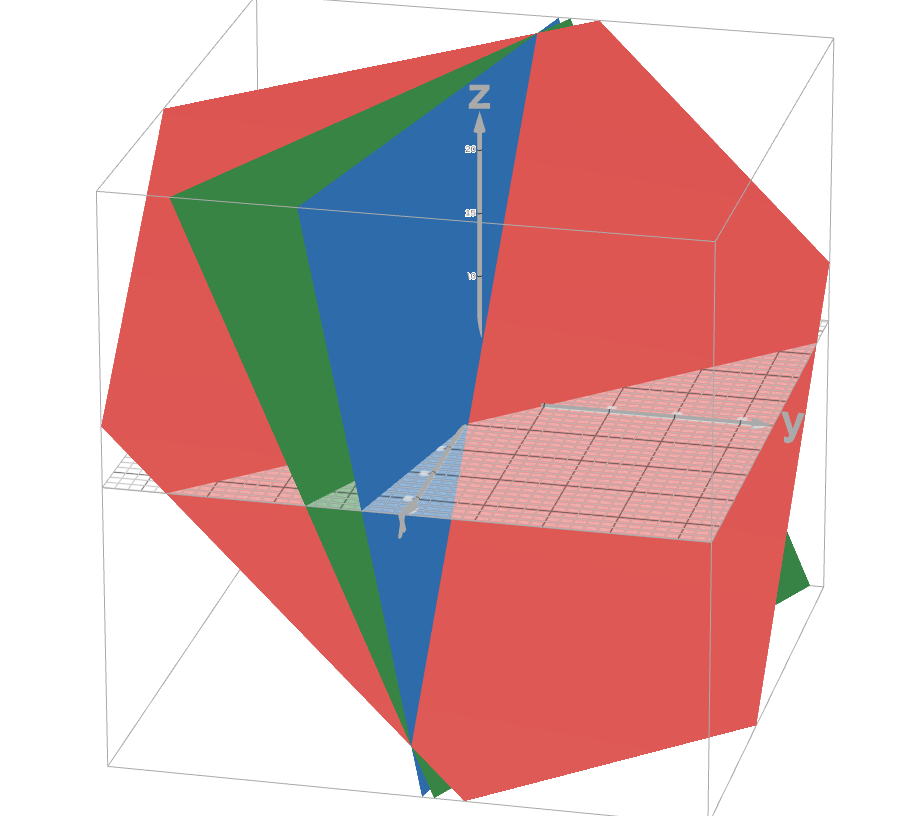
\includegraphics[scale=.15]{images/dependent-system-example}
\end{center}

Hence, the solutions to the system of equations form a line. The third plane
in our system failed to to cut the line of intersection down to a single
point. The equation $E_{3}$ didn't impose any additional restrictions on the
solution set that weren't already imposed by $E_{1}$ and $E_{2}$. This is
because $E_{3}=2E_{1}+E_{2}$. In some sense, $E_{3}$ is just $E_{1}$ and
$E_{2}$ in disguise.

Indeed, if we row reduce, we get a row of zeros:
\begin{align*}
  \begin{augmentedmatrix}{ccc|c}
    1&1&1&5\\
    1&5&1&6\\
    3&7&3&16
  \end{augmentedmatrix}
           \overset{R_{3}-R_{2} \to R_{3}}{\longrightarrow}
  \begin{augmentedmatrix}{ccc|c}
    1&1&1&5\\
    1&5&1&6\\
    2&2&1&10
  \end{augmentedmatrix}
           \overset{R_{3}-2R_{1} \to R_{3}}{\longrightarrow}
  \begin{augmentedmatrix}{ccc|c}
    1&1&1&5\\
    1&5&1&6\\
    0&0&0&0
  \end{augmentedmatrix}
\end{align*}
This implies that the solutions of the system can be expressed as the
intersection of only the first two planes.

How can we predict exactly when this will happen? To understand exactly when a
linear system yields exactly one solution vs.~infinitely many solutions, we
need the concept of ``linear independence''.

\subsection{Linear independence}
\begin{definition}
  Let $V$ be a vector space and let $v_{1},\ldots,v_{n}\in V$. We say that the
  set $\left\{v_{1},\ldots,v_{n}\right\}$ is \demph{linearly dependent} if
  there are scalars $c_{1},c_{2},\ldots,c_{n}$ \textit{not all zero} such that
  \begin{equation*}
    c_{1}v_{1}+c_{2}v_{2}+\ldots+c_{n}v_{n} = \vec{0}.
  \end{equation*}
  If the vectors $v_{1},\ldots,v_{n}$ are not linearly dependent, we say that
  they are \demph{linearly independent.}
\end{definition}

Geometrically, we can visualize linear dependence in the following way.  For
vectors in 3-dimensional space, two vectors are linearly dependent if they lie
on the same line. \textit{Three vectors are linearly dependent if they lie in the same
plane.}


\begin{example}
  Are the vectors
  \begin{equation*}
    \begin{bmatrix}
      1\\2\\3
    \end{bmatrix},
    \begin{bmatrix}
      3\\2\\1
    \end{bmatrix},
    \begin{bmatrix}
      -1\\2\\5
    \end{bmatrix}
  \end{equation*}
  linearly dependent or linearly independent?

  To determine the answer we need to solve the
  linear system, to see if there are any solutions other than $c_{1}=c_{2}=c_{3}=0$.
  \begin{equation*}
    \begin{bmatrix}
      1&3&-1\\
      2&2&2\\
      3&1&5
    \end{bmatrix}
    \begin{bmatrix}
      c_1\\c_2\\c_3
    \end{bmatrix}
    =
    \begin{bmatrix}
      0\\0\\0
    \end{bmatrix}
  \end{equation*}
  Row reducing, we get
  \begin{equation*}
    \begin{augmentedmatrix}{cccc}
      1&3&-1&0\\
      2&2&2&0\\
      3&1&5&0
    \end{augmentedmatrix}
    \longrightarrow
    \begin{augmentedmatrix}{cccc}
      1&0&2&0\\
      0&1&-1&0\\
      0&0&0&0
    \end{augmentedmatrix}
  \end{equation*}
  Convert back to equations
  \begin{align*}
    c_{1}+2c_{3}&=0\\
    c_{2}-c_{3}&=0\\
    0&=0
  \end{align*}
  We can write this as
  \begin{align*}
    c_{1}&=-2c_{3}\\
    c_{2}&=c_{3}
  \end{align*}
  with free variable $c_{3}\in \R$. Therefore, there are infinitely many
  solutions. For example, if $c_{3}=1$, we get the solution
  \begin{equation*}
    \begin{bmatrix}
      c_{1}\\c_{2}\\c_{3}
    \end{bmatrix}
    =
    \begin{bmatrix}
      -2\\1\\1
    \end{bmatrix}
  \end{equation*}
  We've shown that there is a nontrivial linear combination of the vectors
  which equals zero. Therefore they are linearly dependent.
\end{example}

\textbf{This example illustrates a general method:} To check any set of
vectors $v_{1},\ldots,v_{n}$ for independence, put them in the colunns of $A$
Then solve the system $Ac=\vec{0}$. The vectors are dependent if there is a
solution other than $c=\vec{0} $



To relate today's discussion of linear independence back to our nexus
question, we utilize our key theorem. Let $A$ be an $n\times n$ matrix, and
let $B\in \R^{n}$ be an arbitrary vector. We wish to know whether the linear
system $AX=B$ has a unique solution or not. (After all, if it has infinitely
many solutions, that means we have at least one redundant equation.)


Then the following statements are equivalent:
\begin{center}
  The columns of $A$ are linearly independent.

  $\Updownarrow$
  
  The only solution to $AX=\vec{0}$ is $X=\vec{0}$.

  $\Updownarrow$

  $A$ is nonsingular
  
  $\Updownarrow$

  The equation $AX=B$ has exactly one solution for any $B\in \R^{n}$. 
\end{center}



\newpage

\newpage
\section{2025-10-01: Week 06 | Lecture 16}

\begin{center}
  \begin{tcolorbox}[width=0.9\textwidth, colback=white, colframe=black]
    \textit{\textbf{The nexus question of this lecture:} How can we build
      linear subspaces from a \textbf{minimal} set of vectors?}
  \end{tcolorbox}
\end{center}

\subsection{Linear Indepdenence}

\begin{definition}
  Let $V$ be a vector space and let $v_{1},\ldots,v_{n}\in V$. We say that the
  set $\left\{v_{1},\ldots,v_{n}\right\}$ is \demph{linearly dependent} if
  there are scalars $c_{1},c_{2},\ldots,c_{n}$ \textit{not all zero} such that
  \begin{equation*}
    c_{1}v_{1}+c_{2}v_{2}+\ldots+c_{n}v_{n} = \vec{0}.
  \end{equation*}
  If the vectors $v_{1},\ldots,v_{n}$ are not linearly dependent, we say that
  they are \demph{linearly independent.}
\end{definition}

\textbf{General method:} To check any set of vectors $v_{1},\ldots,v_{n}$
for independence, put them in the colunns of $A$ Then solve the system
$Ac=\vec{0}$. The vectors are dependent if there is a solution other than
$c=\vec{0} $

\begin{example}
  \label{ex:linear-independence-1}
  Are the vectors
  \begin{equation*}
    \left\{
      \begin{bmatrix}
        1\\0\\1
      \end{bmatrix},
      \begin{bmatrix}
        1\\1\\1
      \end{bmatrix},
      \begin{bmatrix}
        -1\\1\\1
      \end{bmatrix}
    \right\}
  \end{equation*}
  linearly independent?

  \textbf{Solution:}
  We need to check if the linear system
  \begin{equation*}
    \begin{bmatrix}
      1&1&-1\\
      0&1&1\\
      1&1&1
    \end{bmatrix}
    \begin{bmatrix}
      c_{1}\\c_{2}\\c_{3}
    \end{bmatrix}
    =
    \begin{bmatrix}
      0\\0\\0
    \end{bmatrix}
  \end{equation*}
  has any nontrivial solutions.

  Using row reduction, we have
  \begin{equation*}
    \begin{augmentedmatrix}{ccc|c}
      1&1&-1&0\\
      0&1&1&0\\
      1&1&1&0      
    \end{augmentedmatrix}
  \end{equation*}
  can be row reduced to
  \begin{equation*}
    \begin{augmentedmatrix}{ccc|c}
      1&1&-1&0\\
      0&1&1&0\\
      0&0&2&0      
    \end{augmentedmatrix}    
  \end{equation*}
  We could go further, but this is sufficient. Converting back to a system of equations,
  \begin{align*}
    c_{1}+c_{2}-c_{3}&=0 \\
    c_{2}+c_{3}&=0 \\
    2c_{3}&=0 \\
  \end{align*}
  Back substitution gives $c_{1}=c_{2}=c_{3}=0$. Thus, the only solution to
  the linear system is the trival solution. Therefore the set of vectors is
  linearly independent.
\end{example}

\begin{example}
  Show that the columns of the following matrix are linearly independent:
  \begin{equation*}
    \begin{bmatrix}
      3&4&2\\0&1&5\\0&0&2
    \end{bmatrix}
  \end{equation*}
  Look for a linear combination that makes zero:
  
  \begin{equation*}
    c_{1}
    \begin{bmatrix}
      3\\0\\0
    \end{bmatrix}
    +
    c_{2}
    \begin{bmatrix}
      4\\1\\0
    \end{bmatrix}
    +
    c_{3}
    \begin{bmatrix}
      2\\5\\2
    \end{bmatrix}
    =
    \begin{bmatrix}
      0\\0\\0
    \end{bmatrix}
  \end{equation*}
  We need to show that $c_{1},c_{2},c_{3}$ are all forced to be zero.

  Indeed, the third row forces $c_{3}$ to be zero. Then the second row forces
  $c_{2}$ to be zero. Then the first row forces $c_{1}$ to be zero. Hence, the
  columns are linearly independent
\end{example}




\subsection{Basis}
Linear independence allows us to make precise the notion of what it means for
a spaning set of vectors to be minimal. Such a set is called a basis:

\begin{definition}[Basis]
  \label{def:basis}
  Let $V$ be a vector space and let $v_{1},\ldots,v_{n}\in V$. We say that
  $v_{1},\ldots,v_{n}$ are a \demph{basis} for $V$ if both the following
  conditions are satisfied:
  \begin{enumerate}[label=(\roman*.)]
    \item $v_{1},\ldots,v_{n}$ span $V$. 
    \item $v_{1},\ldots,v_{n}$ are linearly independent. 
  \end{enumerate}
\end{definition}
Condition (i.) says that you have enough vectors to generate the linear space
$V$, and condition (ii.) says that \textit{you don't have too many vectors}
(i.e., minimality). To answer the motivating question of the last few
lectures, a basis is a minimal generating set for a linear subspace (which may
include be whole space $V$).

This latter point about minimality is related to the following theorem

\begin{theorem}
  Let $V$ be a vector space, and let $v_{1},\ldots,v_{n}\in V$. Then the
  $v_{1},\ldots,v_{n}$ are linearly dependent if and only if one of the
  $v_{1},\ldots,v_{n}$ is a linear combination of the others.
\end{theorem}


\begin{example}[The standard basis vectors]
  \label{ex:standard-basis-vectors}
  The vectors
  \begin{equation*}
    e_{1}=
    \begin{bmatrix}
      1\\0\\0
    \end{bmatrix}, \quad 
    e_{2}=
    \begin{bmatrix}
      0\\1\\0
    \end{bmatrix}, \quad 
    e_{3}=
    \begin{bmatrix}
      0\\0\\1
    \end{bmatrix}
  \end{equation*}
  are a basis for $\R^{3}$.

  To check this, observe that
  \begin{enumerate}[label=(\roman*.)]
    \item (linear independence) It is clear that equality holds in the equation
    \begin{equation*}
      c_{1}e_{1}+c_{2}e_{2}+c_{3}e_{3}=0
    \end{equation*}
    only if $c_{1}=c_{2}=c_{3}=0$. That is, there is no nontrivial linear
    combination of $e_{1},e_{2},e_{3}$ which equals the zero vector. So
    $e_{1},e_{2},e_{3}$ are linearly independent.
    \item (spanning) If $
    \begin{bmatrix}
      a\\b\\c
    \end{bmatrix}
    $
    is an arbitrary vector in $\R^{3}$, then
    \begin{equation*}
      ae_{1}+be_{2}+ce_{3} =
      \begin{bmatrix}
        a\\b\\c
      \end{bmatrix}
    \end{equation*}
    Therefore $\Span(e_{1},e_{2},e_{3})$ includes every vector in $\R^{3}$.
  \end{enumerate}
\end{example}


\begin{example}
  Show that
  \begin{equation*}
    \begin{bmatrix}
      1\\0\\1
    \end{bmatrix},\quad
    \begin{bmatrix}
      1\\1\\1
    \end{bmatrix},\quad
    \begin{bmatrix}
      -1\\1\\1
    \end{bmatrix}
  \end{equation*}
  form a basis for $\R^{3}$.

  \textbf{Solution:} We already checked that these vectors are linearly
  independent in \cref{ex:linear-independence-1}. To it suffices to show that
  we can write any vector $
  \begin{bmatrix}
    z\\y\\z
  \end{bmatrix}
  $ in $\R^{3}$ as a linear combination of the three vectors.

  To see this, set up the system
  \begin{equation*}
    \begin{bmatrix}
      1&1&-1\\
      0&1&1\\
      1&1&1      
    \end{bmatrix}
    \begin{bmatrix}
      c_{1}\\c_{2}\\c_{3}
    \end{bmatrix}
    =
    \begin{bmatrix}
      x\\y\\z
    \end{bmatrix}.
  \end{equation*}
  If this system always has a solution, then the vectors span $\R^{3}$. If
  there is some vector $ \begin{bmatrix} x\\y\\z \end{bmatrix} $ such that the
  above equation has no solutions, then the vectors do not span $\R^{3}$. We
  can check it by (you guessed it) row reducing.
  
  \begin{equation}\label{eq:1}
    \begin{augmentedmatrix}{ccc|c}
      1&1&-1&x\\
      0&1&1&y\\
      1&1&1&z      
    \end{augmentedmatrix}
    \overset{R_{3}-R_{1}\to R_{3}}{\longrightarrow}
    \begin{augmentedmatrix}{ccc|c}
      1&1&-1&x\\
      0&1&1&y\\
      0&0&2&z-x      
    \end{augmentedmatrix}
    \overset{R_{1}-R_{2} \to R_{1}}{\longrightarrow}
    \begin{augmentedmatrix}{ccc|c}
      1&0&-2&x-y\\
      0&1&1&y\\
      0&0&2&z-x      
    \end{augmentedmatrix}
  \end{equation}
  \begin{equation*}
    \overset{R_{1}+R_{3} \to R_{1}}{\longrightarrow}
    \begin{augmentedmatrix}{ccc|c}
      1&0&0&z-y\\
      0&1&1&y\\
      0&0&2&z-x      
    \end{augmentedmatrix}
    \overset{R_{2}-\frac{1}{2}R_{3} \to R_{2}}{\longrightarrow}
    \begin{augmentedmatrix}{ccc|c}
      1&0&0&z-y\\
      0&1&0&y-\frac{1}{2}(z-x)\\
      0&0&2&z-x      
    \end{augmentedmatrix}
    \overset{\frac{1}{2}R_{3} \to R_{3}}{\longrightarrow}
    \begin{augmentedmatrix}{ccc|c}
      1&0&0&z-y\\
      0&1&0&y-\frac{1}{2}(z-x)\\
      0&0&1&\frac{1}{2}(z-x)
    \end{augmentedmatrix}
  \end{equation*}
  Therefore, the solution is $c_{1} =z-y$, $c_{2} =
  y+\frac{x}{2}-\frac{z}{2}$, $c_{3}= \frac{z}{2}-\frac{x}{2}$. Since this
  solution exists for any $x,y,z$, we have shown that the vectors form a basis.
\end{example}

\newpage
\section{2025-10-03 | Week 06 | Lecture 17}
\textit{Sub lecture by R. Willett.}

\textit{Lecture on section 2.4}

If $V$ is a vector space, a \demph{basis} for $V$ is a collection
$v_{1},\ldots,v_{n}\in V$ such that
\begin{itemize}
  \item  $v_{1},\ldots,v_{n}$ span $V$
  \item $v_{1},\ldots,v_{n}$ are linearly independent
\end{itemize}

\begin{example}[Bases]
  $\R^{3}$ has `standard basis'
  \begin{equation*}
    \begin{bmatrix}
      1\\0\\0
    \end{bmatrix},
    \begin{bmatrix}
      0\\1\\0
    \end{bmatrix},
    \begin{bmatrix}
      0\\0\\1
    \end{bmatrix},
  \end{equation*}
  but there may be others, e.g.,
  \begin{equation*}
    \begin{bmatrix}
      3\\0\\0
    \end{bmatrix},
    \begin{bmatrix}
      4\\1\\0
    \end{bmatrix},
    \begin{bmatrix}
      2\\5\\2
    \end{bmatrix},
  \end{equation*}
  or
  \begin{equation*}
    \begin{bmatrix}
      1\\0\\1
    \end{bmatrix},
    \begin{bmatrix}
      1\\1\\1
    \end{bmatrix},
    \begin{bmatrix}
      -1\\1\\1
    \end{bmatrix},
  \end{equation*}
\end{example}


\begin{example}
  $M_{m\times n}(\R)$ has basis $E_{11},E_{12},\ldots,E_{1n},E_{21}, \ldots,
  E_{2n},\ldots, E_{m1},\ldots E_{mn}$
  where $E_{ij}$ is an $m\times n$ matrix with $1$ at position $(i,j)$ and
  zero else.

  Again, there are others, e.g.
  \begin{equation*}
    \begin{bmatrix}
      1&0\\
      0&-1
    \end{bmatrix},
    \begin{bmatrix}
      1&0\\
      0&1
    \end{bmatrix},
    \begin{bmatrix}
      0&1\\
      1&0
    \end{bmatrix},
    \begin{bmatrix}
      0&-1\\
      1&0
    \end{bmatrix}
  \end{equation*}
\end{example}

\begin{theorem}[Theorem 2.9 in textbook -- not obvious!]
  If $v_{1},\ldots,v_{n}$ and $w_{1},\ldots,w_{m}$ are both bases for the same
  vector space, then $m=n$.
\end{theorem}

\begin{definition}[Dimension]
  \label{def:dimension}
  The \demph{dimension} of a vector space is the number of elements in a
  basis. Notation for the dimension of $V$:
  \begin{equation*}
    \dim(V).
  \end{equation*}
\end{definition}

\begin{example}[Dimension]
  \label{ex:dimension}
  \begin{itemize}
    \item $\dim(\R^{3})=3$ and more generally $\dim(\R^{n})=n$. 
    \item $\dim( \R[x]_{ \leq 2})=3$ and more generally $\dim(\R[x]_{ \leq n})=n+1$
  \end{itemize}
  \textbf{Comments:}
  \begin{itemize}
    \item Some vector spaces have bases with infinitely many vectors (e.g. a
    basis for $\R[x]$ is $1,x,x^{2},x^{3},\ldots$). In this case, the
    dimension of $V$ is infinite. Notation: $\dim(V)=\infty$.

    (In this course, you will mainly focus on finite dimensional vector
    spaces.)
    \item If $V$ is the $0$ vector space, we write $\dim(V)=0$.
  \end{itemize}
\end{example}

\begin{theorem}[Some important properties of dimension (see 2.11 and 2.12)]
  \label{thm:some-important-properties-dimension}
  Let $V$ be a vector space with $\dim(V)=n$. Then
  \begin{enumerate}
    \item [(a)] If $v_{1},\ldots,v_{k}\in V$ are linearly independent, then
    $k \leq n$ and there are $v_{k+1},v_{k+2},\ldots,v_{n}$ with
    $v_{1},\ldots,v_{k},v_{k+1},\ldots,v_{n}$ a basis (``linear independent
    collections cannot be too big'')
    \item [(b)] If $v_{1},\ldots,v_{k}\in V$ span $V$, then $k \geq n$, and some
    collection of $n$ vectors from $v_{1},\ldots,v_{k}$ is a basis
    `(``spanning collections collections cannot be too small'')
  \end{enumerate}
\end{theorem}

\begin{theorem}[Dimension-basis]
  \label{thm:dimension-basis-lemma}
  Suppose $v_{1},\ldots,v_{n}\in V$, where $\dim(V)=n$. Then
  \begin{itemize}
    \item If $v_{1},\ldots v_{n}$ span $V$, then they are a basis.
    \item If $v_{1},\ldots,v_{n}$ are linearly independent, they are a basis.
  \end{itemize}
\end{theorem}
\begin{example}
  Which (if any) of the following collections is a basis for $\R^{3}$?
  \begin{enumerate}[label=(\alph*)]
    \item $
    \begin{bmatrix}
      1\\3\\5
    \end{bmatrix},
    \begin{bmatrix}
      4\\5\\6
    \end{bmatrix}
    $ 
    \item $
    \begin{bmatrix}
      1\\2\\3
    \end{bmatrix},
    \begin{bmatrix}
      4\\5\\6
    \end{bmatrix},
    \begin{bmatrix}
      7\\8\\9
    \end{bmatrix}
    $ 
    \item
    $
    \begin{bmatrix}
      1\\2\\3
    \end{bmatrix},
    \begin{bmatrix}
      4\\5\\6
    \end{bmatrix},
    \begin{bmatrix}
      7\\8\\9
    \end{bmatrix},
    \begin{bmatrix}
      10\\11\\12
    \end{bmatrix}
    $ 
  \end{enumerate}
  \textbf{Solution:}
  \begin{enumerate}%[label=(\alph*)]
    \item [(a)] No: has too few vectors (so cannot span)
    \item [(c)] No: has too many vectors (so cannot be linearly independeent)
    \item [(b)] To check linear independence, we need to check whether
    \begin{equation*}
      c_{1}
      \begin{bmatrix}
        1\\2\\3
      \end{bmatrix}
      +c_{2}
      \begin{bmatrix}
        4\\5\\6
      \end{bmatrix}
      +c_{3}
      \begin{bmatrix}
        7\\8\\9
      \end{bmatrix}
      =
      \begin{bmatrix}
        0\\0\\0
      \end{bmatrix}
    \end{equation*}
    has nontrivial solutions.

    Check linear independence by row reducing:
    \begin{align*}
      \begin{bmatrix}
        1&4&7\\
        2&5&8\\
        3&6&9
      \end{bmatrix}
         & \longrightarrow
           \begin{bmatrix}
             1&4&7\\
             0&-3&-6\\
             0&-6&-12
           \end{bmatrix} &&\text{ $R_{2}-2R_{1}$ and $R_{3}-3R_{1} $ }\\
         & \longrightarrow
           \begin{bmatrix}
             1&4&7\\
             0&-3&-6\\
             0&0&0
           \end{bmatrix} &&\text{ $R_{3}-2R_{2}$ }
    \end{align*}
    As we have a row of zeroes, there are no conditions on $c_{3}$, and we see
    that there are infinitely many solutions.

    We conclude that the collection is not a basis (since it's not linearly
    independent.)
  \end{enumerate}
\end{example}

\subsection{Null space, row space, column space}

Let $A\in M_{m\times n}(\R)$. There are three important vector spaces
associated with $A:$

\begin{itemize}
  \item The \demph{column space}, which is the subspace of $M_{m\times 1}(\R)$
  spanned by the columns of $A$. Notation: $CS(A)$ 
  \item The \demph{row space}, which is the subspace of $M_{1\times n}(\R)$
  spanned by the rows of $A$. Notation $RS(A)$.
  \item The \demph{null space} (aka: kernel) which is the subspace of $R^{n}$
  of vectors $x$ such that $Ax=0$. Notation $NS(A)$ or $\ker(A)$.
\end{itemize}

\newpage
\section{2025-10-06 | Week 07 | Lecture 18}

\begin{center}
  \begin{tcolorbox}[width=0.9\textwidth, colback=white, colframe=black]
    \textit{\textbf{The nexus question of this lecture:} What are the three
      fundamental linear subspaces associated with a matrix $A$?}
  \end{tcolorbox}
\end{center}

\subsection{Three fundamental subspaces}
\begin{definition}[The fundamental subspaces of $A$]
  \label{def:fundamental-subspaces-a}
  Let $A\in M_{m\times n}(\R)$. There are three important vector spaces
  associated with $A:$

  \begin{itemize}
    \item The \demph{column space}, which is the subspace of
    $M_{m\times 1}(\R)$ spanned by the columns of $A$. Notation: $CS(A)$
    \item The \demph{row space}, which is the subspace of $M_{1\times n}(\R)$
    spanned by the rows of $A$. Notation $RS(A)$.
    \item The \demph{null space} which is the subspace of $R^{n}$ of vectors
    $x$ such that $Ax=0$. Notation $NS(A)$. The nullspace and the kernel are
    the same thing.
  \end{itemize}
\end{definition}

\begin{remark}[Connection between column space and matrix multiplication]
  The idea of column space is natural. If
  \newcommand*{\vertbar}{\rule[-1ex]{0.5pt}{2.5ex}}
  \newcommand*{\horzbar}{\,\rule[.5ex]{2.5ex}{0.5pt}\,}
  \begin{equation*}
    A = 
    \left[
      \begin{array}{cccc}
        \vertbar & \vertbar &        & \vertbar \\
        A_{1}    & A_{2}    & \ldots & A_{n}    \\
        \vertbar & \vertbar &        & \vertbar 
      \end{array}
    \right]\in M_{m\times n}(\R)
  \end{equation*}
  then for any vector $x= (x_{1},\ldots,x_{n})^{\top} \in \R^{n}$
  \begin{equation*}
    Ax = A_{1}x_{1}+A_{2}x_{2}+\ldots+A_{n}x_{n}
  \end{equation*}
  This is linear combination of the columns of $A$, so the output $Ax$ is
  always an element of the column space. Another word for column space is the
  \demph{image} or \demph{range} of the [linear transformation of the] matrix $A$.
\end{remark}


\begin{definition}[rank]
  The \demph{rank} of a matrix is the dimension of its column space (= dim of
  row space).
\end{definition}


\begin{theorem}
  For $A\in M_{m\times n}(\R)$, the dimensions satisfy
  \begin{equation*}
    \dim RS(A) = \dim CS(A)
  \end{equation*}
  and
  \begin{equation*}
    \underbrace{\dim CS(A)}_{\text{`rank'}} + \underbrace{\dim
      NS(A)}_{\text{`nullity'}} = \underbrace{n}_{\text{\# cols of }A}
  \end{equation*}
\end{theorem}
The second part is called the rank-nullity theorem. Noting that
$\mathrm{rank}(A)=\dim CS(A)$ and that $NS(A) = \ker(A)$, we have




\subsection{Some examples of computing bases for the three fundamental subspaces}
\begin{example}[Row space, column space, null space]
  \label{ex:row-space-column-space-null-space}
  Let
  \begin{equation*}
    A =
    \begin{bmatrix}
      1&0&-1&3\\
      2&1&4&-1\\
      4&1&2&5
    \end{bmatrix}
    \in M_{3\times 4}(\R).
  \end{equation*}
  Find bases for
  \begin{enumerate}
    \item[(a)] $RS(A)$
    \item[(b)] $NS(A)$
  \end{enumerate}
  \textbf{Solution}
  \begin{enumerate}
    \item[(a)] Wrong:
    \begin{equation*}
      \begin{bmatrix}1&0&-1&3\end{bmatrix},
      \begin{bmatrix}2&1&4&-1\end{bmatrix},
      \begin{bmatrix}4&1&2&5\end{bmatrix}
    \end{equation*}
    Better approach:
    
    \textit{Idea: row reduction does not change row space, so row reduce until we get
      a linearly independent set.}

    The reduced row echelon form is
    \begin{equation}\label{eq:4}
      A_{\rm RREF} = \begin{bmatrix}
        1&0&-1&3\\
        0&1&6&-7\\
        0&0&0&0
      \end{bmatrix}
    \end{equation}
    A basis of $A_{\rm RREF}$ is
    \begin{equation*}
      \begin{bmatrix}1&0&-1&3 \end{bmatrix},\
      \begin{bmatrix}0&1&6&7 \end{bmatrix}
    \end{equation*}
    (since these are linearly independent). Moreover, we note that since row
    reduction doesn't change the row space,
    \begin{equation*}
      RS(A)= RS(A_{\rm RREF}).
    \end{equation*}
    and hence
    \begin{equation*}
      \begin{bmatrix}1&0&-1&3 \end{bmatrix},\
      \begin{bmatrix}0&1&6&7 \end{bmatrix}
    \end{equation*}
    are a basis for $RS(A)$ as well.
    
    \item [(b)] We will use the fact that
    \begin{equation*}
      NS(A) = NS(A_{\rm RREF}).
    \end{equation*}
    So it suffices to find a basis for $NS(A_{\rm RREF})$. Let's do a
    computation to sese what $NS(A_{\rm RREF})$ looks like. Recall that
    $NS(A_{\rm RREF})$ consists of the vectors $x$ satisfying
    \begin{equation}\label{eq:5}
      A_{\rm RREF}x = 0
    \end{equation}
    If $x=(x_{1},\ldots,x_{5})^{\top}$ satisfies \cref{eq:5}, then we have
    \begin{equation*}
      \begin{bmatrix}
        1&0&-1&3\\
        0&1&6&-7\\
        0&0&0&0
      \end{bmatrix}
      \begin{bmatrix}
        x_{1}\\x_{2}\\x_{3}\\x_{4}
      \end{bmatrix}
      =
      \begin{bmatrix}
        0\\0\\0\\0
      \end{bmatrix}.
    \end{equation*}
    Writing this as equations, we have
    \begin{align*}
      x_{1}-x_{3}+3x_{4}&=0\\
      x_{2}+6x_{3}-7x_{4}&=0\\
                        0&=0.
    \end{align*}
    Therfore we have:
    \begin{align*}
      x_{1} &= x_{3}-3x_{4}\\
      x_{2} &= -6x_{3}+7x_{4}
    \end{align*}
    where $x_{3},x_{4}$ are free variables.
    
    Therefore if $x\in RS(A_{\rm RREF})$ (equivlently, if $x$ satisfies
    \cref{eq:5}), then it has the following form
    \begin{equation*}
      \begin{bmatrix}
        x_{1}\\x_{2}\\x_{3}\\x_{4}
      \end{bmatrix}
      =
      \begin{bmatrix}
        x_{3}-3x_{4}\\
        -6x_{3}+7x_{4}\\
        x_{3}\\
        x_{4}
      \end{bmatrix}
      = x_{3}
      \begin{bmatrix}
        1\\-6\\0\\1
      \end{bmatrix}
      + x_{4}
      \begin{bmatrix}
        -3\\7\\0\\1
      \end{bmatrix}.
    \end{equation*}
  \end{enumerate}
  This shows that the vectors
  \begin{equation*}
    \begin{bmatrix}
      1\\-6\\0\\1
    \end{bmatrix}
    ,
    \begin{bmatrix}
      -3\\7\\0\\1
    \end{bmatrix}
  \end{equation*}
  span $NS(A)$. Moreover, they are also linearly independent (since two
  vectors are linearly dependent if and only if they are multiples of each
  other, which these are clearly not). Therefore
  \begin{equation*}
    \begin{bmatrix}
      1\\-6\\0\\1
    \end{bmatrix}
    ,
    \begin{bmatrix}
      -3\\7\\0\\1
    \end{bmatrix}
  \end{equation*}
  form a basis for $NS(A_{\rm RREF})$. Since $NS(A_{\rm RREF})=NS(A)$, they
  are a basis for $NS(A)$ as well. Since there are two vectors in the basis,
  $\dim NS(A)=2$.
\end{example}

\newpage



\newpage
\section{2025-10-08 | Week 07 | Lecture 19}
\textit{Topics: section 2.4 - fundamental subspaces, rank nullity, rank, and
  dimension}

\subsection{An alternative characterization of linear dependence
}
The following theorem gives us another quite useful characterization of linear
dependence:

\begin{theorem}
  Let $V$ be a vector space, and let $v_{1},\ldots,v_{n}\in V$. Then the
  $v_{1},\ldots,v_{n}$ are linearly dependent if and only if one of the
  $v_{1},\ldots,v_{n}$ is a linear combination of the others.
\end{theorem}
% \begin{proof}
%   Suppose $v_{1},\ldots,v_{n}$ are linearly dependent. Then there are
%   $c_{1},\ldots,c_{n}\in \R$ not all zero such that
%   \begin{equation*}
%     c_{1}v_{1}+c_{2}v_{2}+\ldots+c_{n}v_{n}=0
%   \end{equation*}
%   We know that at least one of the $c_{i}$'s is nonzero. By possibly renaming
%   the vectors, we may assume that $c_{1}\neq 0$. Then rearranging the above
%   equation, we have
%   \begin{equation*}
%     v_{1} = \left(-\frac{c_{2}}{c_{1}}\right)v_{2}+ \left(-\frac{c_{3}}{c_{1}}\right)v_{3}+\ldots+ \left(-\frac{c_{n}}{c_{1}}\right)v_{n}
%   \end{equation*}
%   Thus $v_{1}$ is a linear combination of the other vectors.

%   Now, let's prove the converse. Suppose that $v_{1}$ is a linear combination
%   of $v_{2},\ldots,v_{n}$. Then there exists constants $c_{2},\ldots,c_{n}$
%   (not the same as before) such that
%   \begin{equation*}
%     v_{1} = c_{2}v_{2}+\ldots+c_{n}v_{n}
%   \end{equation*}
%   and hence
%   \begin{equation*}
%     (-1)v_{1}+c_{2}v_{2}+\ldots+c_{n}v_{n} =0
%   \end{equation*}
%   And this shows that $v_{1},\ldots,v_{n}$ are linearly dependent.
% \end{proof}
Taking $n=2$ in the above theorem gives a useful consequence: two $u,v$, are
linearly dependent if and only if they are scalar multiples of each other.

For example, the vectors $  \begin{bmatrix}
  1\\2\\3
\end{bmatrix},
\begin{bmatrix}
  3\\6\\9
\end{bmatrix}.
$ are scalar multiples of each other, and
hence are dependent. On the other hand, the vectors $  \begin{bmatrix}
  1\\2\\3
\end{bmatrix},
\begin{bmatrix}
  3\\6\\10
\end{bmatrix}.
 $ are not scalar multiples of each other, so they are linearly independent.


\subsection{Rank-Nullity Theorem}

\begin{definition}[Rank]
  The \demph{rank} of a matrix $A$, denoted $\text{rank}(A)$, is the dimension
  of the column space of $A$. That is,
  \begin{equation*}
    \text{rank}(A) = \dim CS(A) \ \ (= \dim RS(A))
  \end{equation*}
\end{definition}

\begin{theorem}[Rank-nullity]
  \label{thm:rank-nullity}
  Let $A$ be an $m\times n$ matrix. Then
  \begin{equation*}
    \underbrace{\dim CS(A)}_{\mathrm{rank}(A)} + \underbrace{\dim NS(A)}_{\mathrm{nullity(A)}} = n
  \end{equation*}
\end{theorem}
% \begin{proof}
%   \begin{align*}
%     \text{rank}(A)
%     &= \dim RS(A) &&\text{by definition }\\
%     &\overset{*}{=} \left( \text{\# of nonzero rows in RREF} \right)\\ 
%     &= \left( \text{\# of nonfree variables in solution of } Ax=0 \right)\\ 
%     &= n- \left( \text{\# of free variables in solution of } Ax=0\right)\\ 
%     &= n - \dim \ker(A)
%   \end{align*}

%   The second equality marked $*$ follows because (1) row operations preserve the row space
%   (i.e. the span of the rows does not change when we do row operations), and
%   because (2) in RREF, the nonzero rows are a basis for the row space (they
%   are linearly independent and span it)

%   % The equality marked $**$ follows because, after row reduction, the rows that
%   % are zero impose no restrictions on the corresponding variables
% \end{proof}


\subsection{More examples of computing bases for the three fundamental
  subspaces}
\begin{example}[\cref{ex:row-space-column-space-null-space} continued]
  Consider the matrix
  \begin{equation*}
    A =
    \begin{bmatrix}
      1&0&-1&3\\
      2&1&4&-1\\
      4&1&2&5
    \end{bmatrix}
    \in M_{3\times 4}(\R).
  \end{equation*}

  Previously, we showed the following:

  \begin{itemize}
    \item The vectors
    $\begin{bmatrix}1&0&-1&3 \end{bmatrix},\
    \begin{bmatrix}0&1&6&7 \end{bmatrix}$
    form a basis for $RS(A)$. Hence, $\dim RS(A)=2$.

    \item The vectors
    $\begin{bmatrix}
      1\\-6\\0\\1
    \end{bmatrix}
    ,
    \begin{bmatrix}
      -3\\7\\0\\1
    \end{bmatrix} $
    form a basis for $NS(A)$. Hence $\dim NS(A)=2$.
  \end{itemize}
  \textbf{Question:} What is $\text{rank}(A)$? In other words, what is
  $\dim CS(A)$?

  \Fl{Solution 1 (general method):} \textit{Idea: to find the column space, take
  the transpose, row-reduce to find a basis for $RS(A^{\top})$, then transpose
  back.}

  \begin{equation*}
    A^{\top} =
    \begin{bmatrix}
      1&2&4\\
      0&1&1\\
      -1&4&2\\
      3&-1&5
    \end{bmatrix}
    \overset{\text{row reduction}}{\longrightarrow}
    \begin{bmatrix}
      1&2&4\\
      0&1&1\\
      0&0&0\\
      0&0&0
    \end{bmatrix}.
  \end{equation*}
  Thus, the vectors
  \begin{equation*}
    \begin{bmatrix}
      1&2&4
    \end{bmatrix}
    ,
    \begin{bmatrix}
      0&1&1
    \end{bmatrix}
  \end{equation*}
  form a basis for $RS(A^{\top})$. Transposing back, it follows that the vectors
  $\begin{bmatrix}
    1\\2\\4
  \end{bmatrix},
  \begin{bmatrix}
    0\\1\\1
  \end{bmatrix}$
  form a basis for $CS(A)$. Since there are two vectors in the basis, it
  follows that $\dim CS(A)=2$.
  
  \Fl{Solution 2:} By the Rank-Nullity Theorem (\cref{thm:rank-nullity}),
  we have
  \begin{equation*}
    \dim CS(A) + \dim NS(A) = 4
  \end{equation*}
  Since $\dim NS(A)=2$ (because 2 vectors in the basis), it follows that
  \begin{equation*}
    \dim CS(A) = 2.
  \end{equation*}

  \Fl{Solution 3:} In the last lecture, we showed that $\dim RS(A) =2$. Recall
  that $\text{rank}(A) := \dim CS(A) = \dim RS(A)$. Therefore $\dim CS(A)=2$.
  

\end{example}


\begin{example}
  Find the column space of
  \begin{equation*}
    A =
    \begin{bmatrix}
      1&1&2\\
      -1&1&0\\
      0&1&1
    \end{bmatrix}.
  \end{equation*}

  \Fl{Solution:} We will again use the general method for finding the column
  space from the previous example. The three steps are: (1) take the transpose,
  (2) row-reduce to find a basis for $RS(A^{\top})$, then (3) transpose back.

  We row reduce $A^{\top}$ which gives
  \begin{equation*}
    A^{\top} =
    \begin{bmatrix}
      1&-1&0\\
      1&1&1\\
      2&0&1
    \end{bmatrix}
    \overset{\text{row reduction}}{\longrightarrow}
    \begin{bmatrix}
      1&-1&0\\
      0&2&1\\
      0&0&0
    \end{bmatrix}.
  \end{equation*}
  The nonzero rows are a basis for $R(A^{\top})$. Transposing back, we have
  \begin{equation*}
    \begin{bmatrix}
      1\\-1\\0
    \end{bmatrix}
    \quad \text{and} \quad
    \begin{bmatrix}
      0\\2\\1
    \end{bmatrix}
  \end{equation*}
  This is a basis for the colum space of $A$. 
\end{example}


\subsection{Connection between rank and invertibility}

\begin{theorem}
  \label{thm:rank-invertibiility}
  Let $A$ be an $n\times n$ matrix. Then $A$ is invertible if and only if
  $\text{rank}(A)=n$.
\end{theorem}

One way to see why this is true involves thinking of $A$ as a transformation
of $n$-dimensional space $\R^{n}$. Observe that
\begin{itemize}
  \item $A$ is non-invertible exactly when the transformation collapses the dimension.
  \item The rank of $A$ is the dimension of its range (since range = 
  column space).
  \item So if $\text{rank}(A)<n$ then a dimension collapse occurs, in which
  case $A$ is not invertible. But if $\text{rank}(A)=n$, then no dimension
  collapse occurs, so $A$ is invertible in that case.
\end{itemize}


Thus, \cref{thm:rank-invertibiility} gives another condition we can add to our
key theorem.

\newpage
\section{2025-10-10 | Week 07 | Lecture 20}

\begin{center}
  \begin{tcolorbox}[width=0.9\textwidth, colback=white, colframe=black]
    \textit{\textbf{The nexus question of this lecture:} What is a linear transformation?}
  \end{tcolorbox}
\end{center}

\textit{This lecture is based on section 5.1 in the textbook.w}

\subsection{Function notation}

When a function $f$ goes from a set $X$ to a set $Y$, we write
\begin{equation*}
  f:X \to Y
\end{equation*}
which is read as ``$f$ maps $X$ to $Y$''. The set $X$ is the \demph{domain} of
$f$. The set $Y$ is the \demph{codomain} of $f$. The subset
\begin{equation*}
  \mathrm{Range}(f) = \left\{f(x)\mid x\in X\right\} 
\end{equation*}
is called the \demph{range} of $f$.

\begin{example}
  \begin{itemize}
    \item Let $f(x) = e^{x}$. Then $f: \R \to \R$. The range of this function is the
    set of positive real numbers.
    \item Let $g: \R^{2} \to \R$ ge given by
    \begin{equation*}
      g \left(
        \begin{bmatrix}
          x\\y
        \end{bmatrix}
      \right)  = x^{2}-y^{2}
    \end{equation*}
    The range of the function is $\R$, which is the same as its codomain.
  \end{itemize}
\end{example}

\subsection{Linear Transformation}
\begin{definition}
  Let $V,W$ be vector spaces and $T:V \to W$ a function. We say that $T$ is a
  \demph{linear transformation} if, for all vectors $u,v\in V$ and $c\in \R$,
  we have
  \begin{enumerate}[label=(\roman*)]
    \item $T(u+v)= T(u)+T(v) $ \quad (preserves addition)
    \item $T(cV)= cT(v)$.  \quad (preserves scalar multiplication)
  \end{enumerate}
  Sometimes people refer to linear transformations as \demph{linear
    operators}, which means the same thing.
\end{definition}

You have seen linear transformations before, even if you didn't call them that
at the time. For example, the derivative operator $\frac{d}{dx}$ is one such
function.

\begin{example}
  \label{ex:derivative-is-a-linear-transformation}
  Let $P= \left\{ \text{all polynomials in the variable }x\right\}$. So an
  arbitary element of $P$ looks like
  \begin{equation*}
    p = c_{0}+c_{1}x+c_{2}x^{2}+\ldots+c_{r}x^{r}
  \end{equation*}
  for some nonnegative integer $r$.
  
  We know that $P$ is a vector space. Define a function
  \begin{equation*}
    T: P \to P
  \end{equation*}
  where $T(p) = p'$. In other words, $T= \frac{d}{dx}$.

  To check that $T$ is a linear transformation, let $p,q\in P$ and $c\in \R$. Then
  \begin{itemize}
    \item $T(p+q) = \frac{d}{dx}\left[ p(x)+q(x) \right]= p'(x)+q'(x) =
    T(p)+ T(q)$. 
    \item $T(cp)= \frac{d}{dx}\left[ cp(x) \right]= c \frac{d}{dx} \left[ p(x)
    \right] = c T(p)$.
  \end{itemize}
\end{example}

\begin{example}
  Let $T:\R^{3}\to \R^{2}$ be ggiven by
  \begin{equation*}
    T
    \begin{bmatrix}
      x\\y\\z
    \end{bmatrix}
    =
    \begin{bmatrix}
      x+y-z\\
      x+2y+x
    \end{bmatrix}
  \end{equation*}
  we can check that this is also a linear transformation.

  First observe that we can write
  \begin{equation*}
    T
    \begin{bmatrix}
      x\\y\\z
    \end{bmatrix}
    =
    \begin{bmatrix}
      1&1&-1\\
      1&2&1
    \end{bmatrix}
    \begin{bmatrix}
      x\\y\\z
    \end{bmatrix}.
  \end{equation*}
  Letting $A =  \begin{bmatrix}
    1&1&-1\\
    1&2&1
  \end{bmatrix}$, we can write
  \begin{equation*}
    T(v) = Av, \text{ for }v\in \R^{3}.
  \end{equation*}
  Let's check conditions (i) and (ii) in the definition of linear transformation:
  \begin{itemize}
    \item Proof of (i): Let $u,v\in \R^{3}$. Then
    \begin{equation*}
      T(u+v) = A(u+v) = Au+Av = T(u)+T(v)
    \end{equation*}
    This shows that condition (i) holds. 
    \item Proof of (ii): Let $c\in \R$ and $u\in \R^{3}$. Then
    \begin{equation*}
      T(cu )= A(cu) = c(Au) = cT(u)
    \end{equation*}
    This shows that condition (ii) holds.
  \end{itemize}
  Therefore since both conditions are met, $T$ is a linear transformation.
\end{example}

The proofs from the previous example didn't depend on the specific
form of $A$, only that $A$ was a matrix. Thus we have the following theorem:

\begin{theorem}
  If $A$ is an $m\times n$ matrix, then the function $T: \R^{n}\to \R^{m}$
  given by
  \begin{equation*}
    T(X) = AX
  \end{equation*}
  is a linear transformation.
\end{theorem}

Linear transformations of this form are called \demph{matrix transformations}.


\begin{theorem}
  Suppose $T:V \to W$ is a linear transformation. Then
  \begin{enumerate}[label=(\roman*)]
    \item $T(0)=0$.
    \item For any vectors $v_{1},\ldots,v_{n}\in V$ and scalars
    $c_{1},\ldots,c_{n}\in \R$, we have
    \begin{equation*}
      T(c_{1}v_{1}+\ldots+c_{n}v_{n})=
      c_{1}T(v_{1})+\ldots+c_{n}T(v_{n})
    \end{equation*}
  \end{enumerate}
\end{theorem}
The second property says that linear transformations preserve linear
combinations.
\begin{proof}
  To show that $T(0)=0$ involves a trick. Observe that
  \begin{equation*}
    T(0) = T(0+0) = T(0)+T(0).
  \end{equation*}
  Subtracting $T(0)$ from both sides gives
  \begin{equation*}
    T(0)=0.
  \end{equation*}

  Proof of (ii) is omitted, but follows from the definition of linear
  transformation. (HW?)
\end{proof}

\begin{definition}
  The \demph{kernel} of a linear transformation $T:V \to W$ the set
  \begin{equation*}
    \ker(T) = \left\{v\in V : T(v) = 0\right\} 
  \end{equation*}
\end{definition}
The previous theorem shows that $0$ is always in $\ker(T)$. Just like
matrices. Huh.


\begin{example}
  Let $T: \R^{3}\to \R^{3}$ be the linear transformation defined by
  \begin{equation*}
    T
    \begin{bmatrix}
      x\\y\\z
    \end{bmatrix}
    :=
    \underbrace{\begin{bmatrix}
      1&1&-1\\
      1&2&1
    \end{bmatrix}}_{A}
    \begin{bmatrix}
      x\\y\\z
    \end{bmatrix}.
  \end{equation*}
  \Fl{Question:} Find a basis for $\ker(T)$. [Equivalently: find a basis for $NS(A)$.]

  \Fl{Solution:} \textit{Idea: solve the homogeneous system $AX=0$, then
    interpret the solution.}

  The system $AX=0$ is
  \begin{equation*}
    \begin{bmatrix}
      1&1&-1\\1&2&1
    \end{bmatrix}
    \begin{bmatrix}
      x\\y\\z
    \end{bmatrix}
    =
    \begin{bmatrix}
      0\\0
    \end{bmatrix}.
  \end{equation*}
  We can solve this with row reduction:
  \begin{equation*}
    \begin{augmentedmatrix}{ccc|c}
      1&1&-1&0\\
      1&2&1&0
    \end{augmentedmatrix}
    \overset{\text{row reduction}}{\longrightarrow}
    \begin{augmentedmatrix}{ccc|c}
      1&0&-3&0\\
      0&1&2&0
    \end{augmentedmatrix}.
  \end{equation*}
  This corresponds to the equations
  \begin{equation*}
    \left\{ \begin{array}{l@{}l} x-3z=0 \\ y+2z=0 \end{array}\right.
  \end{equation*}
  or
  \begin{equation*}
    \left\{ \begin{array}{l@{}l} x=3z \\ y=-2z \end{array}\right.
  \end{equation*}
  where $z$ a free variable. Thus, every solution $X=
  \begin{bmatrix}
    x\\y\\z
  \end{bmatrix}
  $ to $AX=0$ takes the form
  \begin{equation*}
    \begin{bmatrix}
      3z\\-2z\\z
    \end{bmatrix} =
    \begin{bmatrix}
      3\\-2\\1
    \end{bmatrix}z
  \end{equation*}
  Therefore the vector $
  \begin{bmatrix}
    3\\-2\\1
  \end{bmatrix}
  $ form a basis for $\ker(T)$.
\end{example}



\newpage
\section{2025-10-13 | Week 08 | Lecture 21}
\begin{center}
  \begin{tcolorbox}[width=0.9\textwidth, colback=white, colframe=black]
    \textit{\textbf{The nexus question of this lecture:} Is a basis all you need? }
  \end{tcolorbox}
\end{center}

\textit{This lecture is based on sections 5.1 and 2.4}

\subsection{All you need is a basis}
If we know how a linear transformation acts on a basis, then we know its
values on all other vectors as well.

\begin{example}[Cool example]
  \label{ex:cool-example}
  Suppose that $T: \R^{3}\to \R^{2}$ is a linear transformation.

  Note that the vectors
  \begin{equation*}
    \begin{bmatrix}
      1\\1\\0
    \end{bmatrix},
    \begin{bmatrix}
      0\\1\\1
    \end{bmatrix},
    \begin{bmatrix}
      1\\0\\1
    \end{bmatrix}
  \end{equation*}
  form a basis of $\R^{3}$. (Check this).

  Suppose that $T$ is defined for each of these three basis vectors as
  \begin{equation*}
    T
    \begin{bmatrix}
      1\\1\\0
    \end{bmatrix} :=
    \begin{bmatrix}
      2\\3
    \end{bmatrix},
    \quad
    T
    \begin{bmatrix}
      0\\1\\1
    \end{bmatrix}
    :=
    \begin{bmatrix}
      0\\3
    \end{bmatrix},
    \quad \text{and} \quad 
    T
    \begin{bmatrix}
      1\\0\\1
    \end{bmatrix}
    :=
    \begin{bmatrix}
      0\\2
    \end{bmatrix}.
  \end{equation*}

  \Fl{Question:} What is $T \begin{bmatrix} 1\\3\\0 \end{bmatrix}$?

  \fl{Solution:} First, we will write $
  \begin{bmatrix}
    1\\3\\0
  \end{bmatrix}
  $ as a linear combination of the basis vectors. To do this, we solve the linear system
  \begin{equation*}
    c_{1}
    \begin{bmatrix}
      1\\1\\0
    \end{bmatrix}
    +
    c_{2}
    \begin{bmatrix}
      0\\1\\1
    \end{bmatrix}
    +
    c_{3}
    \begin{bmatrix}
      1\\0\\1
    \end{bmatrix}
    =
    \begin{bmatrix}
      1\\3\\0
    \end{bmatrix}
  \end{equation*}
  which gives these unique solution $c_{1}=2$, $c_{2}=1$, $c_{3}=-1$.

  Then
  \begin{align*}
    T
    \begin{bmatrix}
      1\\3\\0
    \end{bmatrix}
    &=
      T \left(
      2
      \begin{bmatrix}
        1\\1\\0
      \end{bmatrix}
    +
    \begin{bmatrix}
      0\\1\\1
    \end{bmatrix}
    -
    \begin{bmatrix}
      1\\0\\1
    \end{bmatrix}
    \right)\\ 
    &=2T
      \begin{bmatrix}
        1\\1\\0
      \end{bmatrix}
    + T
    \begin{bmatrix}
      0\\1\\1
    \end{bmatrix}
    - T
    \begin{bmatrix}
      1\\0\\1
    \end{bmatrix}\\
    &=
      2
      \begin{bmatrix}
        2\\3
      \end{bmatrix}
    +
    \begin{bmatrix}
      0\\3
    \end{bmatrix}
    -
    \begin{bmatrix}
      0\\2
    \end{bmatrix}=
      \begin{bmatrix}
        4\\7
      \end{bmatrix}.
  \end{align*}
  We could ask the same question for an arbitrary matrix, namely, what is
  $T \begin{bmatrix}
    x\\y\\z
  \end{bmatrix}
  $? See pg 237-238 in the textbook.
\end{example}

This example shows that if we how a linear transform acts on a basis, then we
know everything about it. This suggests that there is something very special
about a basis, that it's a way to represent a vector space as a whole using
just a finite set of vectors.

\subsection{Unique basis representations}


\begin{theorem}[Unique basis representation]
  \label{thm:unique-basis-representation}
  Let $V$ be a vector space and let $v_{1},\ldots,v_{n}$ be a basis for $V$.
  Then every vector can be written as a unique linear combination
  of $v_{1},\ldots,v_{n}$.
\end{theorem}
\begin{proof}
  Let $u\in V$ be arbitrary. Since $v_{1},\ldots,v_{n}$ is a basis, it spans
  $V$. Therefore we can write $u$ as a linear combination
  \begin{equation}\label{eq:2}
    u = c_{1}v_{1}+c_{2}v_{2}+\ldots+c_{n}v_{n}
  \end{equation}
  for some $c_{1},\ldots,c_{n}\in \R$. This shows that $u$ can be written as a
  linear combination of $v_{1},\ldots,v_{n}$.

  It remains to show that there is only one way to write $u$ as a linear
  combination of $v_{1},\ldots,v_{n}$.

  Suppose we have some \textit{other} linear combination
  \begin{equation}\label{eq:3}
    u = c_{1}'v_{1}+c_{2}'v_{2}+\ldots+c_{n}'v_{n}
  \end{equation}
  where $c_{1}',\ldots,c_{n}\in \R$. Then
  \begin{align*}
    0 
    &= u-u\\
    &= \left(  c_{1}v_{1}+c_{2}v_{2}+\ldots+c_{n}v_{n} \right) - \left(  c_{1}'v_{1}+c_{2}'v_{2}+\ldots+c_{n}'v_{n} \right)\\ 
    &= (c_{1}-c_{1}')v+(c_{2}-c_{2}')v+\ldots+ (c_{n}-c_{n}')v
  \end{align*}
  Since $v_{1},\ldots,v_{n}$ are linearly independent, it follows that
  \begin{equation*}
    c_{1}=c_{1}', \quad c_{2}=c_{2}',\quad \ldots \quad c_{n}=c_{n}'
  \end{equation*}
  So the two linear combinations in \cref{eq:2,eq:3} are actually the same.
  This shows uniqueness.
\end{proof}

One consequence of \cref{thm:unique-basis-representation} is that it allows us
to translate any $n$-dimensional vector space, no matter how exotic, to the
more familiar setting of $\R^{n}$. The idea is as follows:
\begin{enumerate}
  \item Let $V$ be an abstract vector space (functions, polynomials, whatever)
  of dimension $n$.
  \item Pick a basis $v_{1},\ldots,v_{n}$ for $V$
  \item Each $a\in V$ can be written as
  \begin{equation*}
    a_{1}v_{1}+a_{2}v_{2}+\ldots+a_{n}v_{n}
  \end{equation*}
  where $a_{1},\ldots,a_{n}\in \R$. In particular,
  \cref{thm:unique-basis-representation} tells us that there is only one
  choice of $a_{1},\ldots,a_{n}$ that work. So we can write
  \begin{equation*}
    a =
    \begin{bmatrix}
      a_{1}\\
      a_{2}\\
      \vdots\\
      a_{n}
    \end{bmatrix}
  \end{equation*}
\end{enumerate}
In other words, any $n$-dimensional vector space is just $\R^{n}$ in disguise.
So from one perpsective, to study all (finite-dimensional) vector spaces, it's
enough to just study $\R^{n}$.

But there's a catch. Doing this requires ``picking'' a basis---and if you and
I pick different bases, then we will end up with different representations of
the same fundamental objects. Consider the set of direction vectors that an
electron could move. Clearly this ``is'' $\R^{3}$, but since there are no
coordinate axes, we need to \textit{choose} what the $x,y,z$ directions are: I
can just declare that a particular direction is the $x$ direction, for
example. But if you choose a different direction, then we'll end up with
different ways of representing the same directions. My $
\begin{bmatrix}
  1\\2\\0
\end{bmatrix} 
$ might be your $
\begin{bmatrix}
  5\\-3\\2
\end{bmatrix}
$. This may be undesirable.

If you and I each choose different basis for $\R^{3}$, are we really studying
the same space? Maybe we are (I think so!). This is because many properties in
linear algebra are ``basis invariant'' in the sense that they don't depend on
the basis you pick. An example is the dimension of a vector space or its
linear subspaces. Another example is linear transformations: many geometric
properties of linear transformations (e.g., whether they preserve orientation,
how much they stretch space, whether they collapse the dimesnion) don't depend
on how we choose to represent the space. But if that's the case, then maybe we
shouldn't need to rely on picking bases to study these things.

So my answer to the nexus question, ``is a basis all you need'' is ``mostly
yes, but sometimes it's more than than you need.''

\newpage
\section{2025-10-15 | Week 08 | Lecture 22}
\begin{center}
  \begin{tcolorbox}[width=0.9\textwidth, colback=white, colframe=black]
    \textit{\textbf{The nexus question of this lecture:} Why do the row space
      and column space always have the same dimension?}
  \end{tcolorbox}
\end{center}
\textit{This lecture is based on sections 5.1}

\subsection{The dimension of the column space equals the dimension of the row space}

Consider the $3\times 2$ matrix
\begin{equation*}
  \begin{bmatrix}
    1&1\\
    0&0\\
    0&0
  \end{bmatrix}
\end{equation*}
The row space is the vector space $\left\{
  \begin{bmatrix}
    x&x
  \end{bmatrix}
  : x\in \R
\right\}$.
The column space is the vector space $\left\{
  \begin{bmatrix}
    x\\0\\0
  \end{bmatrix}: x\in \R
\right\}$. These are not the same. But they have the same dimesnion: 1.

The fact that the dimensions are equal is not a coincidence.

\begin{theorem}
  Given any $m\times n$ matrix $A$, the row space and column space always have
  the same dimesion. That is, $\dim RS(A)=\dim CS(A)$.
\end{theorem}

\subsection{Preliminaries}

We begin with the following theorem.
\begin{theorem}
  \label{thm:ker-range-subspace}
  Let $X,Y$ be vector spaces.
  If $T: X \to Y$ is a linear transformation, then $\ker(T)$ is a subspace
  of $X$ and $\range(T)$ is a subspace of $Y$.
\end{theorem}
\begin{proof}
  The fact that $\ker(T)$ is a subspace follows similarly to the proof of
  \cref{thm:kernels-are-subspaces} (the ``kernels are subspaces'' theorem from
  lecture 13).

  To show that $\range(T)$ is a subspace of $Y$, we need only verify two
  facts:
  \begin{enumerate}[label=(\roman*)]
    \item $y+y'\in \range(T)$ whenever $y,y'\in \range(T) $
    \item $cy\in\range(T)$ whenever  $y\in Y$ and $c\in \R$
  \end{enumerate}
  \begin{itemize}
    \item \textbf{Proof of (i).} Let $y,y'\in Y$. Then there exist $x,x'$
    such that $T(x)=y$ and $T(x')=y'$. Since $X$ is closed under vector
    addition, $x+x'\in X$. Moreover,
    \begin{equation*}
      T(x+x')= T(x)+T(x')=y+y'
    \end{equation*}
    Therefore $y+y'\in \range(T)$.
    \item \textbf{Proof of (ii).} Let $y\in \range(T).$ Then there exists $x\in
    X$ such that $T(x)=y$. Therefore
    \begin{align*}
      cy 
      &= cT(x)\\
      &= T(cx)
    \end{align*}
    Since $X$ is closed under scalar multiplication $cx\in X$. Therefore
    $cy\in \range(T)$.
  \end{itemize}
\end{proof}
Because $\ker(T),\range(T)$ are subspaces by \cref{thm:ker-range-subspace},
they each have bases, a fact which we will need to use to prove the following theorem.

\subsection{Rank-nullity, again}
\begin{theorem}[Rank Nullity Theorem -- Theorem 5.4 in textbook]
  \label{thm:rank-nullity-theorem-theorem-5.4-textbook}
  If $T:V \to W$ is a linear transformation where $V$ is a finite dimensional
  vector space, then
  \begin{equation*}
    \dim \ker(T) + \dim \range(T) = \dim V
  \end{equation*}
  If $T$ is an $m\times n$ matrix $A$, then $A:\R^{n}\to R^{m}$, and we can
  restate this as
  \begin{equation}\label{eq:6}
    \dim NS(A) + \dim CS(A) = n
  \end{equation}
  (recall that the column space is the range, and that nullspace and kernel
  are synonyms).
\end{theorem}
\begin{proof}[Proof sketch]
  Suppose $\dim \ker(T)=k$ and $\dim V =n$ (note: $k \leq n$). Then with some
  work (omitted, see p242), one can find vectors $v_{1},\ldots, v_{n}\in V$ which form a
  basis for $V$ with the property that
  \begin{itemize}
    \item $v_{1},\ldots,v_{k}$ is a basis for $\ker(T)$; and,
    \item
    $\underbrace{T(v_{k+1}),T(v_{k+1}),\ldots, T(v_{n})}_{n-k\text{ vectors}}$
    is a basis for $\range(T)$.
  \end{itemize}
  This shows that $\dim \range(T) = n-k$. Therefore we have:
  \begin{itemize}
    \item $\dim \ker(T)=k$
    \item $\dim \range(T) = n-k$ 
    \item $\dim V =n$
  \end{itemize}
  Putting these together implies
  \begin{equation*}
    \dim \ker(T) + \dim \range(T) = \dim(V). 
  \end{equation*}
\end{proof}
\subsection{Dimension of the nullspace}
\begin{theorem}
  \label{thm:dim-of-nullspace-is-n-r}
  Let $A$ be an $n\times m$ matrix. Then
  \begin{equation*}
    \dim NS(A) = n-r,
  \end{equation*}
  where $r=\dim RS(A)$.
\end{theorem}
An example will illustrate why \cref{thm:dim-of-nullspace-is-n-r} is true.
Suppose we have a $4\times 5$ matrix $A$ and we want to solve the linear
system $AX=0$. Suppose that row-reducing the augmented matrix gives
\begin{equation*}
  \begin{augmentedmatrix}{ccccc|c}
    1&0&2&3&4&0\\
    0&1&5&6&7&0\\
    0&0&0&0&0&0\\
    0&0&0&0&0&0\\
  \end{augmentedmatrix}
\end{equation*}
This has two nonzero zero rows after row-reduction, so $r=2$.
\cref{thm:dim-of-nullspace-is-n-r} says that
\begin{equation*}
  \dim NS(A)=n-r=5-2=3.
\end{equation*}
We can check this. The augmented matrix above corresponds to the linear system
\begin{align*}
  x_{1}+2x_{3}+3x_{4}+4x_{5}&=0\\
  x_{2}+5x_{3}+6x_{4}+7x_{5}&=0
\end{align*}
or
\begin{align*}
  x_{1}&=-2x_{3}-3x_{4}-4x_{5}\\
  x_{2}&=-5x_{3}-6x_{4}-7x_{5}
\end{align*}
and this has three free variables $x_{3},x_{4},x_{5}$. Therefore the solutions
to $AX=0$ are of the form
\begin{equation*}
  \begin{bmatrix}
    -2x_{3}-3x_{4}-4x_{5}\\
    -5x_{3}-6x_{4}-7x_{5}\\
    x_{3}\\
    x_{4}\\
    x_{5}
  \end{bmatrix}
  =
  x_{3}
  \begin{bmatrix}
    -2\\-5\\1\\0\\0
  \end{bmatrix}
  +
  x_{4}
  \begin{bmatrix}
    -3\\-6\\0\\1\\0
  \end{bmatrix}
  +
  x_{5}
  \begin{bmatrix}
    -4\\-7\\0\\0\\1
  \end{bmatrix}
\end{equation*}
Therefore the nullspace has dimension 3 because
\begin{equation*}
  NS(A) = \Span \left\{
    \begin{bmatrix}
      -2\\-5\\1\\0\\0
    \end{bmatrix}
    \begin{bmatrix}
      -3\\-6\\0\\1\\0
    \end{bmatrix}
    \begin{bmatrix}
      -4\\-7\\0\\0\\1
    \end{bmatrix}
  \right\}.
\end{equation*}

\subsection{Proof that $\dim CS(A)=\dim RS(A)$}

We can now prove the following theorem, which says that the row space and
column space of a matrix are the same thing.
\begin{theorem}
  \label{thm:rowspace-columnspace-same-dimension}
  If $A$ is any $m\times n$ matrix, then
  \begin{equation*}
    \dim RS(A) = \dim NS(A)
  \end{equation*}
\end{theorem}
\begin{proof}
  By \cref{thm:rank-nullity-theorem-theorem-5.4-textbook},
 \begin{equation}\label{eq:8}
   \dim NS(A) + \dim CS(A)=n.
 \end{equation}
 By \cref{thm:dim-of-nullspace-is-n-r},
 \begin{equation}\label{eq:7}
   \dim NS(A) = n- \dim RS(A)
 \end{equation}
 Plugging \cref{eq:7} into \cref{eq:8} gives
 \begin{equation*}
   n-\dim RS(A)+ \dim CS(A)=n
 \end{equation*}
 wich simplifies to
 \begin{equation*}
   \dim RS(A)=\dim CS(A).
 \end{equation*}
\end{proof}

\cref{thm:rowspace-columnspace-same-dimension} says that we are justified in
writing
\begin{equation*}
  \rank(A) = \dim NS(A) = \dim CS(A)
\end{equation*}
and hence that
\begin{equation*}
  \rank(A) + \mathrm{nullity}(A)=n
\end{equation*}
for any $m\times n$ matrix $A$.

\newpage
\section{2025-10-17 | Week 08 | Lecture 23}
\begin{center}
  \begin{tcolorbox}[width=0.9\textwidth, colback=white, colframe=black]
    \textit{\textbf{The nexus question of this lecture:} Why is matrix
      multiplication defined the way it is?}
  \end{tcolorbox}
\end{center}
\textit{This lecture is based on section 5.2}

\subsection{Combining linear transformations: the geometric perspective}

Let $V,W$ be vector spaces. A \demph{linear transformation} is a function
$T:V \to W$ given by with the property that
\begin{equation*}
  T(av+bv')=aT(v)+bT(v')
\end{equation*}
for any $v,v'\in V$ and $a,b\in \R$.

If $V=\R^{2}$ then linear transformations include things like
\begin{itemize}
  \item rotations about the origin
  \item reflections across any line of the form $y=mx$
  \item projections of the plane onto a line of the form $y=mx$
  \item uniform stretching of space
  \item any shearing of the plane (i.e., which slants the plane)
  \item any combinations of these
\end{itemize}
(The story is similar for higher dimensions, but we get some weirder
transformations: for example in $\R^{4}$, one can rotate space about two axes
at once.)

The last bullet---that we can combine linear transformations---is significant.
In math-speak, let
\begin{equation*}
  S,R:\R^{2}\to \R^{2}
\end{equation*}
be linear transformations. If we first apply the transformation $S$ and then
apply $R$, the resulting transformation of space is the function composition
$R\circ S$.
\begin{example}
  For example, the following matrix rotates space clockwise about the origin
  by $30^{\circ}$ (i.e., $\pi/6$ radians):
  \begin{equation*}
    R
    =
    \begin{bmatrix}
      \cos(\pi/6) & \sin(\pi/6)\\
      -\sin(\pi/6)& \cos(\pi/6)
    \end{bmatrix}
    =
    \begin{bmatrix}
      \frac{\sqrt{3}}{2} & \frac{1}{2}\\
      -\frac{1}{2} & \frac{\sqrt{3}}{2}
    \end{bmatrix}
  \end{equation*}
  and the following matrix stretches space in the $x$-direction by a factor of
  $2$:
  \begin{equation*}
    S =
    \begin{bmatrix}
      2&0\\
      0&1
    \end{bmatrix}
  \end{equation*}

  Then rotating and then stretching is achieved by doing $S$ and then $R$.
  That is, by $R\circ S$. I claim this is given by the matrix product
  \begin{equation*}
    RS =
    \begin{bmatrix}
      \frac{\sqrt{3}}{2} & \frac{1}{2}\\
      -\frac{1}{2} & \frac{\sqrt{3}}{2}
    \end{bmatrix}
    \begin{bmatrix}
      2&0\\
      0&1
    \end{bmatrix}
    =
    \begin{bmatrix}
      \sqrt{3}& \frac{1}{2}\\
      -1 & \frac{\sqrt{3}}{2}
    \end{bmatrix}
  \end{equation*}
  \textbf{The core idea of this lecture is that matrix multiplication is
    defined in such a way that this always happens: i.e., that the product
    $RS$ corresponds to doing transformation $S$ and then doing transformation
    $T$.}

  In other words, the idea of composing linear transformations comes first.
  The reason why people defined matrix multiplication the way it is, is
  because they wanted it to represent composition of linear functions. We make
  this idea more precise in the next section.
\end{example}





\subsection{Matrix multiplication is composition of linear transformations}

Recall that if $f:X \to Y$ and $g:Y \to Z$ are functions, we define the
copmosition $g\circ f$ as
\begin{equation*}
  g\circ f(x) := g(f(x)), \ x\in X.
\end{equation*}
Function composition can be thought of a form of ``multiplication'' (sort of).

\begin{theorem}[Composition of linear transformations]
  \label{thm:composition-linear-transformations}
  If $T:V \to W$ and $S:W \to U$ are linear transformations, then the
  composite function $ST=S\circ T$ is a linear transformation $ST:V \to U$ is
  a linear transformation.
\end{theorem}

\begin{claim}
  \label{claim:matrix-representation}
  Every linear transformation can be represented by a matrix.
\end{claim}
\begin{claimproof}
  This is the subject of the next lecture.
\end{claimproof}


\begin{theorem}
  When we compose linear transformations $T$ and $S$, this corresponds to
  multiplying their matrices.
\end{theorem}

We will prove the case of $2\times 2$ matrices. For a proof of the general
case (which holds for any matrices), see Theorem 5.10 in the textbook (p
258).

\begin{proof}
  Suppose $T,S:\R^{2}\to \R^{2}$ are linear transformations. By
  \cref{claim:matrix-representation} both
  $T$ and $S$ can be represented by $2\times 2$ matrices. That is, there exist
  $a,b,c,d,A,B,C,D\in \R$ such that
  \begin{equation*}
    T
    \begin{bmatrix}
      x\\y
    \end{bmatrix}
    :=
    \begin{bmatrix}
      a&b\\
      c&d
    \end{bmatrix}
    \begin{bmatrix}
      x\\y
    \end{bmatrix}
    =
    \begin{bmatrix}
      ax+by\\
      cx+dy
    \end{bmatrix}
    \quad \text{and} \quad
    S
    \begin{bmatrix}
      x\\y
    \end{bmatrix}
    :=
    \begin{bmatrix}
      A&B\\
      C&D
    \end{bmatrix}
    \begin{bmatrix}
      x\\y
    \end{bmatrix}
    =
    \begin{bmatrix}
      Ax+By\\
      Cx+Dy
    \end{bmatrix}.
  \end{equation*}
  The matrix product is
  \begin{equation*}
    \begin{bmatrix}
      A&B\\
      C&D
    \end{bmatrix}
    \begin{bmatrix}
      a&b\\
      c&d
    \end{bmatrix}
    =
    \underbrace{
      \begin{bmatrix}
      Aa+Bc&Ab+Bd\\
      Ca+Dc&Cb+Dd
    \end{bmatrix}}_{\text{call this }M}
  \end{equation*}
   
  To show that $S\circ T$ corresponds exactly to matrix multiplication, we
  need to show that
  \begin{equation}\label{eq:9}
    S\circ T \left(
      \begin{bmatrix}
      x\\y
    \end{bmatrix}
  \right) 
     =
    M
    \begin{bmatrix}
      x\\y
    \end{bmatrix}
  \end{equation}
  for all $
  \begin{bmatrix}
    x\\y
  \end{bmatrix}\in \R^{2}.
  $
  This is because left-hand side of the above equation is the composition $S\circ T$. The
  right hand side is the product of the matrices for $S$ and $T$. By showing
  that the equality holds, we will show that they are the same thing.
  
  Indeed, 
  \begin{align*}
    S\circ T \left(
    \begin{bmatrix}
      x\\y
    \end{bmatrix}
    \right)
    &=
    S \left( T
    \begin{bmatrix}
      x\\y
    \end{bmatrix}
    \right)\\
    &=S \left(
      \begin{bmatrix}
        ax+by\\cx+dy
      \end{bmatrix}
    \right)\\ 
    &=
      \begin{bmatrix}
        A(ax+by)+B(cx+dy)\\
        C(ax+by)+D(cx+dy)
      \end{bmatrix}\\
    &=
      \begin{bmatrix}
        (Aa+Bc)x+(Ab+Bd)y\\
        (Ca+Dc)x+(Cb+Dd)y
      \end{bmatrix}\\
    &= M
      \begin{bmatrix}
        x\\y
      \end{bmatrix}.
  \end{align*}
  We have demonstrated that \cref{eq:9} holds. We are done. :)
\end{proof}
\newpage

\section{2025-10-20 | Week 09 | Lecture 24}
\begin{center}
  \begin{tcolorbox}[width=0.9\textwidth, colback=white, colframe=black]
    \textit{\textbf{The nexus question of this lecture:} How do we find a
      matrix to represent a linear transformation?}
  \end{tcolorbox}
\end{center}
\textit{This lecture is based on section 5.2 and 5.3}


\subsection{The algebra of linear transformations}

\subsubsection{Algebraic operations}
Let $V$ and $W$ be vector spaces. Consider two linear transformations $T:V \to
W$ and $S:V \to W$. The function $T+S$ is defined as
\begin{equation*}
  (T+S)(v) := T(v)+S(v), \ v\in V
\end{equation*}
And for $c\in \R$, $cT$ is defined as
\begin{equation*}
  (cT)(v):=cT(v),\ v\in V
\end{equation*}

\begin{theorem}
  \label{thm:linear-combinations-of-linear-transformations}
  If $T,S:V \to W$ are linear transformations, then so are $T+S$ and $cT$.
  % More generally, if $T_{1},\ldots,T_{n}:V \to W$ are
  % linear transformations and $c_{1},\ldots,c_{n}\in \R$, then
  % \begin{equation*}
  %   c_{1}T_{1}+c_{2}T_{2}+\ldots+c_{n}T_{n}
  % \end{equation*}
  % is also a linear transformation.
\end{theorem}

In other words, the set of linear transformations $T:V\to W$ is closed under
addition and scalar multiplication. This suggests that set of linear
transformations from $V$ to $W$ forms a vector space. (It does. The rabbit
hole goes deep...)


\begin{example}
  Suppose
  
  \begin{equation*}
    S
    \begin{bmatrix}
      x\\y
    \end{bmatrix}
    :=
    \begin{bmatrix}
      2x-y\\x+2y
    \end{bmatrix}
    \quad \text{and} \quad 
    T
    \begin{bmatrix}
      x\\y
    \end{bmatrix}
    :=
    \begin{bmatrix}
      x+y\\x-y
    \end{bmatrix}
  \end{equation*}
\end{example}
\fl{Question 1: What is $S+3T$?}

\begin{align*}
  (S+3T)\left(
  \begin{bmatrix}
    x\\y
  \end{bmatrix}
  \right) 
  &= S
    \left(\begin{bmatrix}
        x\\y
      \end{bmatrix}\right)
  +3T
  \left(\begin{bmatrix}
      x\\y
    \end{bmatrix}\right)\\
  &=
    \begin{bmatrix}
      2x-y\\
      x+2y
    \end{bmatrix}
  +3
  \begin{bmatrix}
    x+y\\
    x-y
  \end{bmatrix}\\
  &=
    \begin{bmatrix}
      2x-y\\x+2y
    \end{bmatrix}
  +
  \begin{bmatrix}
    3x+3y\\
    3x-3y
  \end{bmatrix}\\
  &=
    \begin{bmatrix}
      5x+2y\\
      4x-y
    \end{bmatrix}
\end{align*}

\fl{Question 2: What is $S\circ T$?}
\begin{align*}
  S\circ T
  \begin{bmatrix}
    x\\y
  \end{bmatrix}
  &=S \left( T
    \begin{bmatrix}
      x\\y
    \end{bmatrix}
  \right)\\ 
  &=S
    \begin{bmatrix}
      x+y\\
      x-y
    \end{bmatrix}\\
  &=
    \begin{bmatrix}
      2(x+y)-(x-y)\\
      (x+y)+2(x-y)
    \end{bmatrix}\\
  &=
    \begin{bmatrix}
      x+3y\\
      3x-y
    \end{bmatrix}
\end{align*}
At this point we note that we can represent
\begin{equation*}
  S
  =
  \begin{bmatrix}
    2&-1\\
    1&2
  \end{bmatrix},
  \quad
  T =
  \begin{bmatrix}
    1&1\\
    1&-1
  \end{bmatrix},
  \quad
  S\circ T
  =
  \begin{bmatrix}
    1&3\\3&-1
  \end{bmatrix},
  \quad
  S+3T
  =
  \begin{bmatrix}
   5&2\\
   4&-1
  \end{bmatrix}
\end{equation*}
Notice that
\begin{equation*}
  \underbrace{
    \begin{bmatrix}
    2&-1\\
    1&2
  \end{bmatrix}}_{S}
\underbrace{
  \begin{bmatrix}
    1&1\\
    1&-1
  \end{bmatrix}}_{T}
  =
  \underbrace{\begin{bmatrix}
    1&3\\
    3&-1
  \end{bmatrix}}_{S\circ T}
  \quad \text{and that} \quad 
  \underbrace{\begin{bmatrix}
    2&-1\\
    1&2
  \end{bmatrix}}_{S}
  + 3
  \underbrace{\begin{bmatrix}
    1&1\\
    1&-1
  \end{bmatrix}}_{T}
  =
  \underbrace{
    \begin{bmatrix}
    5&2\\4&-1
  \end{bmatrix}}_{S+3T}
\end{equation*}

\subsubsection{Algebraic rules}
The standard algebraic rules work with linear transformations:

\begin{theorem}
  Let $R,S,T$ be linear transformations and $c,d\in R$. Then
  \begin{itemize}
    \item $S+T=T+S$
    \item $R+(S+T)=(R+S)+T$
    \item $c(dT)=(cd)T $
    \item $c(S+T)=cS+cT$
    \item $R(ST)=(RS)T$
    \item $R(S+T)=RS+RT$
    \item $(R+S)T=RT+ST$
    \item $c(ST)=(cS)T=S(cT)$
  \end{itemize}
\end{theorem}

Observe the glaring lack of the rule that $ST=TS$, which doesn't hold in
general. In fact, all of the above rules are are identical to the rules for
matrix algebra (i.e., if $S,T,$ and $R$ are matrices).

This makes sense because, as we show in the next section, linear
transformations can be encoded with matrices. 

\subsection{Representing a linear transformation with a matrix}

Let
$T:V \to W$ be a linear transformation.

\fl{Goal:} Find a matrix to represent $T$.

We'll start by choosing a basis for $V$ and $W$. Let
$\alpha = \left\{v_{1},\ldots,v_{n}\right\} $ be a basis for $V$ and
$\beta = \left\{w_{1},\ldots,w_{m}\right\}$ be a basis for $W$.

Following the ideas of \cref{ex:cool-example}, it is enough to understand how
$T$ acts on the basis $v_{1},\ldots,v_{n}$.

Observe that
\begin{itemize}
  \item Every vector in $W$ can be written as a unique linear combination of
  the basis vectors $w_{1},\ldots,w_{m}$ (because these form a basis).
  \item The vectors $T(v_{1}),\ldots,T(v_{n})$ are all vectors in $W$.
\end{itemize}
From these two observations, we can find scalars $a_{ij}\in \R$ such that
\begin{align*}
  T(v_{1}) &= a_{11}w_{1}+a_{21}w_{2}+\ldots+a_{m1}w_{m}\\
  T(v_{2}) &= a_{12}w_{1}+a_{22}w_{2}+\ldots+a_{m2}w_{m}\\
           &\ \vdots\\
  T(v_{n}) &= a_{1n}w_{1}+a_{2n}w_{2}+\ldots+a_{mn}w_{m}.
\end{align*}

We can change notation by writing thes as \demph{coordinate vectors}:
\begin{equation*}
  T(v_{1}) =
  \begin{bmatrix}
    a_{11}\\a_{21}\\\vdots \\a_{m1}
  \end{bmatrix}_{\beta}
  \quad
  T(v_{2}) =
  \begin{bmatrix}
    a_{12}\\a_{22}\\\vdots \\a_{m2}
  \end{bmatrix}_{\beta}
  \quad
  \cdots
  \quad
  T(v_{n}) =
  \begin{bmatrix}
    a_{1n}\\a_{2n}\\\vdots \\a_{mn}
  \end{bmatrix}_{\beta}
\end{equation*}
Here, the subscript $\beta$ indicates that these vectors represent linear
combinations of the basis $\beta=\left\{w_{1},\ldots,w_{m}\right\}$. That is,
we are using the notation
\begin{equation*}
  \begin{bmatrix}
    a_{1i}\\a_{2i}\\\vdots \\a_{mi}
  \end{bmatrix}_{\beta} = a_{1i}w_{1}+a_{2i}w_{2}+\ldots+w_{mi}w_{m}, \quad i=1,\ldots,n.
\end{equation*}


We can then represent $T$ simply as the $m\times n$ matrix
\begin{equation*}
  [T]_{\alpha}^{\beta}=
  \begin{bmatrix}
    a_{11}&a_{12}&\cdots& a_{1n}\\
    a_{21}&a_{22}&\cdots& a_{2n}\\
    \vdots&\vdots&\ddots&\vdots\\
    a_{m1}&a_{m2}&\cdots& a_{mn}
  \end{bmatrix}
\end{equation*}
whose columns are the above vectors. We call this matrix \demph{the matrix of
  $T$ with respect to the bases $\alpha$ and $\beta$.} It is denoted
$[T]_{\alpha}^{\beta}$. 




\begin{example}
  Let $T
  \left(\begin{bmatrix}
      x\\y
    \end{bmatrix}
  \right) =
  \begin{bmatrix}
    x+y\\x-y
  \end{bmatrix}
  $.
  Then we can write $v_{1} =
  \begin{bmatrix}
    1\\0
  \end{bmatrix}
  $
  and $v_{2} =
  \begin{bmatrix}
    0\\1
  \end{bmatrix}
  $.

  Here, we take as our basis $\alpha=\beta=\left\{v_{1},v_{2}\right\}$.
  Observe that
  \begin{itemize}
    \item $T(v_{1})=
    \begin{bmatrix}
      1\\1
    \end{bmatrix}
    $
    \item $T(v_{2})=
    \begin{bmatrix}
      1\\-1
    \end{bmatrix}
    $.
  \end{itemize}
  Then
  \newcommand*{\vertbar}{\rule[-1ex]{0.5pt}{2.5ex}}
  \newcommand*{\horzbar}{\,\rule[.5ex]{2.5ex}{0.5pt}\,}

  \begin{equation*}
    [T]_{\alpha}^{\beta} =
    \begin{bmatrix}
      \begin{array}{cc}
        \vertbar & \vertbar\\
        T(v_{1})    & T(v_{2})\\
        \vertbar & \vertbar \\
      \end{array}
    \end{bmatrix}
    =
    \begin{bmatrix}
      1&1\\
      1&-1
    \end{bmatrix}
  \end{equation*}
  Which makes sense, because
  \begin{equation*}
    T
    \begin{bmatrix}
      x\\y
    \end{bmatrix}
    =
    \begin{bmatrix}
      x+y\\x-y
    \end{bmatrix}
    =
    \begin{bmatrix}
      1&1\\1&-1
    \end{bmatrix}
    \begin{bmatrix}
      x\\y
    \end{bmatrix}.
  \end{equation*}
\end{example}

\newpage


\newpage
\section{2025-10-22 | Week 09 | Lecture 25}
\begin{center}
  \begin{tcolorbox}[width=0.9\textwidth, colback=white, colframe=black]
    \textit{\textbf{The nexus question of this lecture:} The matrix we use to
      represent a linear transformation depends on a choice of bases. How does
      it change when whe choose different bases?}
  \end{tcolorbox}
\end{center}
\textit{This lecture is based on section 5.3 in the textbook}

\subsection{Introduction to change of basis}

The following theorem summarizes the main ideas from the previous lecture.

\begin{theorem}[Change of Basis I]
  \label{thm:change-of-basis-I}
  Let $\mathbb{A}$ and $\mathbb{B}$ be vector spaces. If
  $T: \mathbb{A} \to \mathbb{B}$ is a linear map,
  $\alpha= \left\{\alpha_{1},\ldots,\alpha_{n}\right\}$ is a basis of
  $\mathbb{A}$, and $\beta= \left\{\beta_{1},\ldots,\beta_{m}\right\} $ is a
  basis of $\mathbb{B}$, then we can represent $T$ by the matrix
  \newcommand*{\vertbar}{\rule[-1ex]{0.5pt}{2.5ex}}
  \newcommand*{\horzbar}{\,\rule[.5ex]{2.5ex}{0.5pt}\,}

  \begin{equation*}
    [T]_{\alpha}^{\beta}
       = 
      \left[
        \begin{array}{cccc}
          \vertbar & \vertbar &        & \vertbar \\
          T(\alpha_{1})    & T(\alpha_{2})    & \ldots & T(\alpha_{n})    \\
          \vertbar & \vertbar &        & \vertbar 
        \end{array}
      \right]
    \end{equation*}
    where
    $T(\alpha_{i}) = A\alpha_{i} =
    a_{1i}\beta_{1}+a_{2i}\beta_{2}+\ldots+a_{mi}\beta_{m}$ for each
    $i=1,\ldots,n$.

    (Here, $\alpha_{1},\ldots,\alpha_{n}$ are vectors in $\mathbb{A}$ and
    $\beta_{1},\ldots,\beta_{n}$ are vectors in $\mathbb{B}$.)
\end{theorem}


\begin{example}[Example 1 in Section 5.3]
  \label{ex:example-1-section-5.3}
  Let $T:\R^{3}\to \R^{3}$ be the linear transformation
  \begin{equation*}
    T
    \begin{bmatrix}
      x\\y\\z
    \end{bmatrix}
    =
    \begin{bmatrix}
      5x+z\\
      3x+2y-3z\\
      5x
    \end{bmatrix}
  \end{equation*}
  Let  $\alpha= \left\{e_{1},e_{2},e_{3}\right\}$,
  where
  \begin{equation*}
    e_{1}=\begin{bmatrix}
      1\\0\\0
    \end{bmatrix}, \quad
    e_{2}=\begin{bmatrix}
      0\\1\\0
    \end{bmatrix}, \quad
    e_{3}=\begin{bmatrix}
      0\\0\\1
    \end{bmatrix}.
  \end{equation*}
  Clearly $\alpha$ is a basis of $\R^{3}$.

  \begin{enumerate}[(a)]
    \item \textbf{Question:} Find the matrix of $T$ with respect to the
    standard basis $\alpha$, that is, find $[T]_{\alpha}^{\alpha}$.
    
    \textbf{Solution:} Observe that
    \begin{equation*}
      T(e_{1}) = T
      \begin{bmatrix}
        1\\0\\0
      \end{bmatrix}
      =
      \begin{bmatrix}
        5\\3\\5
      \end{bmatrix}
      =5e_{1}+3e_{2}+5e_{3}
    \end{equation*}
    Similarly,
    \begin{equation*}
      T(e_{2}) =
      \begin{bmatrix}
        0\\2\\0
      \end{bmatrix}
      = 0e_{1}+2e_{2}+0e_{3}
      \quad \text{and} \quad
      T(e_{3})=
      \begin{bmatrix}
        1\\-3\\0
      \end{bmatrix}
      = 1e_{1}-3e_{2}+0e_{3}
    \end{equation*}
    These becomes the columns of the matrix
    \begin{equation*}
      [T]_{\alpha}^{\alpha} =
      \begin{bmatrix}
        5&0&1\\
        3&2&-3\\
        5&0&0
      \end{bmatrix}
    \end{equation*}

    \item \textbf{Question:} Let $\beta=
    \left\{\beta_{1},\beta_{2},\beta_{3}\right\}$, where 
    \begin{equation*}
      \beta_{1} =
      \begin{bmatrix}
        1\\1\\2
      \end{bmatrix},
      \quad
      \beta_{2} =
      \begin{bmatrix}
        1\\-1\\1
      \end{bmatrix},
      \quad
      \beta_{3}=
      \begin{bmatrix}
        1\\1\\1
      \end{bmatrix}.
    \end{equation*}
    This is a basis of $\R^{3}$. Find $[T]_{\beta}^{\beta}$, the matrix of
    $T$ with respect to the basis $\beta$.

    \textit{(The point of this
      example is to show you how to find $[T]_{\beta}^{\beta}$ mechanistically;
      I'm not trying to illustrate why this particular choice of basis $\beta$
      is good or meaningful---it's not.)}

    \textbf{Solution:} The columns of $[T]_{\beta}^{\beta}$ are the vectors
    $T(\beta_{1}),T(\beta_{2}),T(\beta_{3})$ expressed in terms of the vectors
    in $\beta$. By plugging $\beta_{1},\beta_{2},\beta_{3}$ into $T$, we see that
    \begin{equation*}
      T(\beta_{1}) =
      \begin{bmatrix}
        7\\-1\\5
      \end{bmatrix},
      \quad
      T(\beta_{2}) =
      \begin{bmatrix}
        6\\-2\\5
      \end{bmatrix},
      \quad
      T(\beta_{3}) =
      \begin{bmatrix}
        6\\2\\5
      \end{bmatrix}
    \end{equation*}
    But in the above equations, the right hand sides are all expressed in
    terms of $e_{1},e_{2},e_{3}$. For example,
    \begin{equation*}
      T(\beta_{1}) =
      \begin{bmatrix}
        7\\-1\\5
      \end{bmatrix}
      =7e_{1}-e_{2}+5e_{3}.
    \end{equation*}
    This is no good: we
    need to express them using in basis $\beta$. Observe that
    \begin{itemize}
      \item $T(\beta_{1})
      =
      \begin{bmatrix}
        7\\-1\\5
      \end{bmatrix}
      \overset{*}{=}
      -2
      \underbrace{\begin{bmatrix}
          1\\1\\2
        \end{bmatrix}}_{\beta_{1}}
      +4
      \underbrace{\begin{bmatrix}
          1\\-1\\1
        \end{bmatrix}}_{\beta_{2}}
      +5
      \underbrace{\begin{bmatrix}
          1\\1\\1
        \end{bmatrix}}_{\beta_{3}}
      =
      -2\beta_{1}+4\beta_{2}+5\beta_{3}=
      \begin{bmatrix}
        -2\\4\\5
      \end{bmatrix}_{\beta}
      $

      Similarly,
      
      \item  $T(\beta_{2})
      =
      \begin{bmatrix}
        6\\-2\\5
      \end{bmatrix}
      \overset{*}{=}
      -1
      \underbrace{\begin{bmatrix}
          1\\1\\2
        \end{bmatrix}}_{\beta_{1}}
      +4
      \underbrace{\begin{bmatrix}
          1\\-1\\1
        \end{bmatrix}}_{\beta_{2}}
      +3
      \underbrace{\begin{bmatrix}
          1\\1\\1
        \end{bmatrix}}_{\beta_{3}}
      =
      \begin{bmatrix}
        -1\\4\\3
      \end{bmatrix}_{\beta}
      $
      \item  $T(\beta_{3})
     =
      \begin{bmatrix}
        6\\2\\5
      \end{bmatrix}
      \overset{*}{=}
      -1
      \underbrace{\begin{bmatrix}
          1\\1\\2
        \end{bmatrix}}_{\beta_{1}}
      +2
      \underbrace{\begin{bmatrix}
          1\\-1\\1
        \end{bmatrix}}_{\beta_{2}}
      +5
      \underbrace{\begin{bmatrix}
          1\\1\\1
        \end{bmatrix}}_{\beta_{3}}
      =
      \begin{bmatrix}
        -1\\2\\5
      \end{bmatrix}_{\beta}
      $
    \end{itemize}

    Therefore by \cref{thm:change-of-basis-I}
    \newcommand*{\vertbar}{\rule[-1ex]{0.5pt}{2.5ex}}
    \newcommand*{\horzbar}{\,\rule[.5ex]{2.5ex}{0.5pt}\,}
    \begin{equation*}
      [T]_{\beta}^{\beta}
      = 
      \begin{bmatrix}
        \begin{array}{ccc}
          \vertbar & \vertbar &         \vertbar \\
          T(\beta_{1})    & T(\beta_{2})   & T(\beta_{3})    \\
          \vertbar & \vertbar &         \vertbar 
        \end{array}
      \end{bmatrix}
      =
      \begin{bmatrix}
        -2&-1&-1\\
        4&4&2\\
        5&3&5
      \end{bmatrix}
    \end{equation*}
    This matrix represents the same linear transformation, $T$, but now we are
    using $\beta$ as the basis for $\R^{3}$ rather than $\alpha$ as in part (a).
    For some linear transformations, the is a ``best'' basis to use (and often
    it is not the standard basis!)

    There is also a 

    \begin{tcolorbox}[colframe=black, colback=gray!5, arc=2mm, boxrule=0.8pt,
      breakable, title=The starred equalities above,   coltitle=black,colbacktitle=black!10]
      Note that the equalities marked with a $(*)$ required solving a linear
      system. In the $T(\beta_{1})$ case, for example, we needed to solve the
      linear system
      \begin{equation*}
        \begin{bmatrix}
          7\\-1\\5
        \end{bmatrix}
        = c_{1}
        \begin{bmatrix}
          1\\1\\2
        \end{bmatrix}
        +
        c_{2}
        \begin{bmatrix}
          1\\-1\\1
        \end{bmatrix}
        +c_{3}
        \begin{bmatrix}
          1\\1\\1
        \end{bmatrix},
      \end{equation*}
      which has solution $c_{1}=-2$, $c_{2}=4$, $c_{3}=5$.
    \end{tcolorbox}


    
    % \item \textbf{Question:} Let $\beta=
    % \left\{\beta_{1},\beta_{2},\beta_{3}\right\}$ where 
    % \begin{equation*}
    %   \beta_{1} =
    %   \begin{bmatrix}
    %     1\\1\\2
    %   \end{bmatrix},
    %   \quad
    %   \beta_{2} =
    %   \begin{bmatrix}
    %     1\\-1\\1
    %   \end{bmatrix},
    %   \quad
    %   \beta_{3}=
    %   \begin{bmatrix}
    %     1\\1\\1
    %   \end{bmatrix}
    % \end{equation*}
    % This is a basis of $\R^{3}$. Find $[T]_{\alpha}^{\beta}$, the matrix of
    % $T$ with respect to the bases $\alpha$ and $\beta$.

    % \textit{(The point of this
    % example is to show you how to find $[T]_{\alpha}^{\beta}$ mechanistically;
    % I'm not trying to illustrate why this particular choice of basis $\beta$
    % is good or meaningful---it's not.)}

    % \textbf{Solution:} The columns of $[T]_{\alpha}^{\beta}$ are the vectors
    % $T(e_{1}),T(e_{2}),T(e_{3})$ expressed in terms of the $\beta$.
    % \begin{equation*}
    %   T(e_{1}) =
    %   \begin{bmatrix}
    %     5\\3\\1
    %   \end{bmatrix},
    %   \quad
    %   T(e_{2}) =
    %   \begin{bmatrix}
    %     0\\2\\0
    %   \end{bmatrix},
    %   \quad
    %   T(e_{3}) =
    %   \begin{bmatrix}
    %     1\\-3\\0
    %   \end{bmatrix}
    % \end{equation*}
    % Observe that
    % \begin{itemize}
    %   \item $T(e_{1})
    %   =
    %   T \left(
    %     \begin{bmatrix}
    %       1\\0\\0
    %     \end{bmatrix}
    %   \right) 
    %   =
    %   \begin{bmatrix}
    %     5\\3\\1
    %   \end{bmatrix}
    %   \overset{*}{=}
    %   0
    %   \underbrace{\begin{bmatrix}
    %     1\\1\\2
    %   \end{bmatrix}}_{\beta_{1}}
    %   +1
    %   \underbrace{\begin{bmatrix}
    %     1\\-1\\1
    %   \end{bmatrix}}_{\beta_{2}}
    %   +4
    %   \underbrace{\begin{bmatrix}
    %     1\\1\\1
    %   \end{bmatrix}}_{\beta_{3}}
    %   =
    %   \begin{bmatrix}
    %     0\\1\\4
    %   \end{bmatrix}_{\beta}
    %   $
    %   \item  $T(e_{2})
    %   =
    %   T \left(
    %     \begin{bmatrix}
    %       0\\1\\0
    %     \end{bmatrix}
    %   \right) 
    %   =
    %   \begin{bmatrix}
    %     0\\2\\0
    %   \end{bmatrix}
    %   \overset{*}{=}
    %   0
    %   \underbrace{\begin{bmatrix}
    %       1\\1\\2
    %     \end{bmatrix}}_{\beta_{1}}
    %   -1
    %   \underbrace{\begin{bmatrix}
    %       1\\-1\\1
    %     \end{bmatrix}}_{\beta_{2}}
    %   +1
    %   \underbrace{\begin{bmatrix}
    %       1\\1\\1
    %     \end{bmatrix}}_{\beta_{3}}
    %   =
    %   \begin{bmatrix}
    %     0\\-1\\1
    %   \end{bmatrix}_{\beta}
    %   $
    % \item  $T(e_{3})
    %   =
    %   T \left(
    %     \begin{bmatrix}
    %       0\\0\\1
    %     \end{bmatrix}
    %   \right) 
    %   =
    %   \begin{bmatrix}
    %     1\\-3\\0
    %   \end{bmatrix}
    %   \overset{*}{=}
    %   -1
    %   \underbrace{\begin{bmatrix}
    %       1\\1\\2
    %     \end{bmatrix}}_{\beta_{1}}
    %   +2
    %   \underbrace{\begin{bmatrix}
    %       1\\-1\\1
    %     \end{bmatrix}}_{\beta_{2}}
    %   +0
    %   \underbrace{\begin{bmatrix}
    %       1\\1\\1
    %     \end{bmatrix}}_{\beta_{3}}
    %   =
    %   \begin{bmatrix}
    %     -1\\2\\0
    %   \end{bmatrix}_{\beta}
    %   $
    % \end{itemize}

    
    % \begin{tcolorbox}[colframe=black, colback=gray!5, arc=2mm, boxrule=0.8pt,
    %   breakable, title=The starred equalities,   coltitle=black,colbacktitle=black!10]
    %   Note that the equalities marked with a $(*)$ required solving a linear
    %   system. In the $T(e_{1})$ case, for example, we needed to solve the
    %   linear system
    %   \begin{equation*}
    %     \begin{bmatrix}
    %       5\\3\\5
    %     \end{bmatrix}
    %     = c_{1}
    %     \begin{bmatrix}
    %       1\\1\\2
    %     \end{bmatrix}
    %     +
    %     c_{2}
    %     \begin{bmatrix}
    %       1\\-1\\1
    %     \end{bmatrix}
    %     +c_{3}
    %     \begin{bmatrix}
    %       1\\1\\1
    %     \end{bmatrix},
    %   \end{equation*}
    %   which has solution $c_{1}=0$, $c_{2}=1$, $c_{3}=4$.
    % \end{tcolorbox}
    % Therefore
    % \begin{equation*}
    %   [T]_{\alpha}^{\beta}
    %   = 
    %   \begin{bmatrix}
    %     \begin{array}{ccc}
    %       \vertbar & \vertbar &         \vertbar \\
    %       T(e_{1})    & T(e_{2})   & T(e_{3})    \\
    %       \vertbar & \vertbar &         \vertbar 
    %     \end{array}
    %   \end{bmatrix}
    %   =
    %   \begin{bmatrix}
    %     0&0&-1\\
    %     1&-1&2\\
    %     4&1&0
    %   \end{bmatrix}
    % \end{equation*}

  \end{enumerate}
\end{example}




\subsection{The change of basis matrix}
Suppose $\alpha=\left\{\alpha_{1},\ldots,\alpha_{n}\right\}$ and
$\beta=\left\{\beta_{1},\ldots,\beta_{n}\right\}$ are bases for the same
vector space $V$.

We can write the vectors of basis $\beta$ in terms of the vectors of basis
$\alpha$:
\begin{align*}
  \beta_{1} &= p_{11}\alpha_{1}+p_{21}\alpha_{2}+\ldots+p_{n1}\alpha_{n}
  \\
  \beta_{2} &= p_{12}\alpha_{1}+p_{22}\alpha_{2}+\ldots+p_{n2}\alpha_{n}\\
            &\ \vdots\\
  \beta_{n} &= p_{1n}\alpha_{1}+p_{2n}\alpha_{2}+\ldots+p_{nn}\alpha_{n}.
\end{align*}
where the $p$'s are all scalars. In other notation, we can write the above
equations as
\begin{equation*} 
  \beta_{1} = \begin{bmatrix}
    p_{11}\\
    p_{21}\\
    \vdots\\
    p_{n1}
  \end{bmatrix}_{\alpha}, \quad
  \beta_{2}=\begin{bmatrix}
    p_{12}\\
    p_{22}\\
    \vdots\\
    p_{n2}
  \end{bmatrix}_{\alpha}, \quad
  \cdots
  \beta_{n}=\begin{bmatrix}
    p_{1n}\\
    p_{2n}\\
    \vdots\\
    p_{nn}
  \end{bmatrix}_{\alpha}.
\end{equation*}
Concatenating these column vectors, we obtain the matrix
\begin{equation*}
  P =
  \begin{bmatrix}
    p_{11}&p_{12}&\cdots& p_{1n}\\
    p_{21}&p_{22}&\cdots& p_{2n}\\
    \vdots&\vdots&\ddots&\vdots\\
    p_{n1}&p_{n2}&\cdots& p_{nn}
  \end{bmatrix}
\end{equation*}
This matrix is called \demph{the change of basis matrix from $\alpha$ to
  $\beta$}.

The following theorem is Corollary 5.13 in the textbook.
\begin{theorem}[Change of basis II]
  \label{thm:change-of-basis-II}
  If $T:V\to V$ is a linear transformation, $\alpha$ and $\beta$ are bases of
  $V$, and $P$ is the change of basis matrix from $\alpha$ to $\beta$, then
  $[T]_{\beta}^{\beta} = P^{-1}[T]_{\alpha}^{\alpha}P.$
\end{theorem}

\begin{example}[Using a change of basis matrix]
  In \cref{ex:example-1-section-5.3}, we had
  \begin{equation*}
    [T]_{\alpha}^{\alpha}=
    \begin{bmatrix}
      5&0&1\\3&2&-3\\5&0&0
    \end{bmatrix}
    \quad \text{and} \quad
    [T]_{\beta}^{\beta}=
    \begin{bmatrix}
      -2&-1&-1\\4&4&2\\5&3&5
    \end{bmatrix}
  \end{equation*}
  One can compute the change of basis matrix $P$ and its inverse $P^{-1}$ for
  $\alpha$ and $\beta$. (For details, see Example 2 pages 260-261.) These are
  \begin{equation*}
    P =
    \begin{bmatrix}
      1&1&1\\
      1&-1&1\\
      2&1&1
    \end{bmatrix}
    \quad \text{and} \quad P^{-1} =
    \begin{bmatrix}
      -1&0&1\\
      1/2&-1/2&0\\
      3/2&1/2&-1
    \end{bmatrix}.
  \end{equation*}
  Thus we could solve part (b) using the formula in
  \cref{thm:change-of-basis-II}:
  \begin{align*}
    [T]_{\beta}^{\beta} 
    &= P^{-1} [T]_{\alpha}^{\alpha}P\\
    &= \begin{bmatrix}
      -1&0&1\\
      1/2&-1/2&0\\
      3/2&1/2&-1
    \end{bmatrix}
               \begin{bmatrix}
                 5&0&1\\
                 3&2&-3\\
                 5&0&0
               \end{bmatrix}
                      \begin{bmatrix}
                        1&1&1\\
                        1&-1&1\\
                        2&1&1
                      \end{bmatrix}\\
    &=\begin{bmatrix}
      -2&-1&-1\\
      4&4&2\\
      5&3&5
    \end{bmatrix}.
  \end{align*}
  This computation agrees with the answer for $[T]_{\beta}^{\beta}$ that we
  obtained in \cref{ex:example-1-section-5.3}.
\end{example}

\newpage
\section{2025-10-24 | Week 09 | Lecture 26}

\begin{center}
  \begin{tcolorbox}[width=0.9\textwidth, colback=white, colframe=black]
    \textit{\textbf{The nexus question of this lecture:} What do linear
      transformations of 2-dimensional space look like?}
  \end{tcolorbox}
\end{center}

\begin{example}[Horizontal and Vertical Dilations]
  Scale space by $a>0$ in the $x$ direction and $b>0$ in the $y$-direction
  \begin{equation*}
    \begin{bmatrix}
      a&0\\
      0&b
    \end{bmatrix}
  \end{equation*}
  This can be undone by
  \begin{equation*}
    \begin{bmatrix}
      \frac{1}{a}&0\\
      0& \frac{1}{b}
    \end{bmatrix}
  \end{equation*}
\end{example}


\begin{example}[Shear]
  \begin{equation*}
    A=\begin{bmatrix}
      1&a\\
      0&1
    \end{bmatrix}
    \quad \text{and} \quad
    B=\begin{bmatrix}
      1&0\\
      b&1
    \end{bmatrix}
  \end{equation*}
  These have inverses
  \begin{equation*}
    A^{-1}=\begin{bmatrix}
      1&-a\\
      0&1
    \end{bmatrix}
    \quad \text{and} \quad
    B^{-1}=\begin{bmatrix}
      1&0\\
      -b&1
    \end{bmatrix} 
  \end{equation*}
  

  \begin{center}
    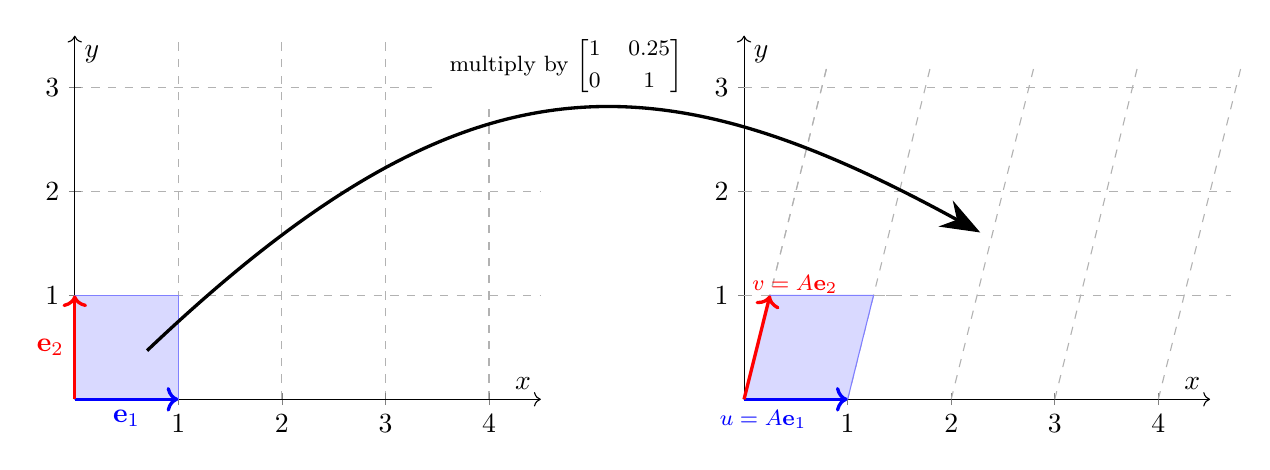
\begin{tikzpicture}
      % --- Left plot ---
      \begin{axis}[
        name=left,
        at={(0,0)}, anchor=south west,
        axis lines=center,
        xmin=0, xmax=4.5,
        ymin=0, ymax=3.5,
        xtick={1,2,3,4},
        ytick={1,2,3},
        xlabel={$x$}, ylabel={$y$},
        axis line style={->},
        width=7.5cm, height=6.2cm,
        clip=false,
        grid=major,
        major grid style={dashed,draw=gray!60}
        ]
        % unit square + unit vectors
        \addplot[fill=blue!15, draw=blue!50] coordinates {(0,0) (1,0) (1,1) (0,1)} -- cycle;
        \addplot[very thick,->,blue] coordinates {(0,0) (1,0)} node[pos=0.5, below] {$\mathbf e_{1}$};
        \addplot[very thick,->,red]  coordinates {(0,0) (0,1)} node[pos=0.5, left] {$\mathbf e_{2}$};
      \end{axis}

      % --- Right plot ---
      \begin{axis}[
        name=right,
        at={(8.5cm,0)}, anchor=south west, % adjust horizontal gap if desired
        axis lines=center,
        xmin=0, xmax=4.5,
        ymin=0, ymax=3.5,
        xtick={1,2,3,4},
        ytick={1,2,3},
        xlabel={$x$}, ylabel={$y$},
        axis line style={->},
        width=7.5cm, height=6.2cm,
        clip=false
        ]
        
        % Define u = Ae1 and v = Ae2
        \def\ux{.25}\def\uy{1}    % u = (0.25,1)
        \def\vx{1}\def\vy{0}    % v = (1,0)

        % --- Custom "grid" aligned with u and v ---
        % Lines parallel to v, offset by k*u   (images of x = k)
        \foreach \k in {1,2,3}{
          \addplot[thin,gray!60,dashed]
          plot[domain=0:4.7, samples=]
          ({x*\vx},{\k*\uy + x*\vy});
        }

        \foreach \k in {1}{
          \addplot[thin,gray!60,dashed]
          plot[domain=0:1.2, samples=2]
          ({\k*\ux + x*\vx},{\k*\uy + x*\vy});
        }

        
        % Lines parallel to u, offset by k*v   (images of y = k)
        \foreach \k in {0}{
          \addplot[thin,gray!60,dashed]
          plot[domain=0:3.2, samples=2]
          ({\k*\vx + x*\ux},{\k*\vy + x*\uy});
        }
        \foreach \k in {0,1,2,3,4}{
          \addplot[thin,gray!60,dashed]
          plot[domain=0:3.2, samples=2]
          ({\k*\vx + x*\ux},{\k*\vy + x*\uy});
        }

        % image of unit square under A: Ae1=(3,1), Ae2=(1,2)
        \addplot[fill=blue!15, draw=blue!50] coordinates {(0,0) (1,0) (1.25,1) (.25,1)} -- cycle;
        \addplot[very thick,->,blue] coordinates {(0,0) (1,0)}
        node[xshift=4pt,pos=0.6, below left] {{\footnotesize $u=A\mathbf e_{1}$}};
        \addplot[very thick,->,red]  coordinates {(0,0) (.25,1)}
        node[xshift=9pt,yshift=4pt,pos=1]  {{\footnotesize$v=A\mathbf e_{2}$}};
      \end{axis}

      % --- Arching arrow + label between plots ---
      \draw[very thick, -{Stealth[length=5mm]}]
      ([xshift=-5cm,yshift=-4cm]left.north east)
      .. controls ($(left.north east)+(-1,-.2)$) and ($(right.north west)+(-1.2,-.2)$) ..
      ([xshift=3cm,yshift=-2.5cm]right.north west)
      node[pos=0.5, above=1pt, fill=white, xshift=3pt, yshift=1pt]
      {{\footnotesize multiply by $\displaystyle \begin{bmatrix}1&0.25\\[2pt]0&1\end{bmatrix}$}};
    \end{tikzpicture}
  \end{center}
  This transformation is a \demph{horizontal shear}. It does not change the
  height of any point. Points above the $x$-axis get shifted right (because
  $a=0.25$ is positive) and points below the $x$-axis get shifted left. The
  further away from the $x$-axis, the greater the horizontal shift. The
  $x$-axis is not changed at all by this transformation---it is
  \demph{invariant} under the linear transformation. This transformation can
  be undone by $
  \begin{bmatrix}
    1&-0.25\\
    0&1
  \end{bmatrix}
  $, which is the inverse.

  The transformation
  \begin{equation*}
    \begin{bmatrix}
      1&0\\
      b&1
    \end{bmatrix}
  \end{equation*}
  is similar, but effectuates a \demph{vertical shear}.
\end{example}


A square matrix $A$ is said to be an \demph{orthogonal matrix} is $A$ and $A^{\top}$ are
inverses.

The determinant of an orthogonal matrix is alwasy $\pm 1$ because
\begin{equation*}
  1 = \det(I)=\det (A^{\top}A) = \det(A^{\top})\det(A) =\left(\det(A)\right)^{2}.
\end{equation*}
Orthogonal matrices has the property that they \textit{preserve distances},
i.e., that
\begin{equation*}
  \dist(x,y) = \dist(Ax,Ay).
\end{equation*}
In words, if you choose any two points, their distance doesn't change under
the linear transformation---the points may get sent to new coordinates, but
the distance between them doesn't change.

If $A$ is an orthogonal matrix and $\det(A)=1$, then we say that $A$ is a
\demph{rotation}.



\begin{example}[Rotation]
  Let $R_{\theta}:\R^{2}\to \R^{2}$ be a rotation of the plane about origin by
  $\theta$ radians counterclockwise. This linear transformation is represented
  by the matrix
  \begin{equation*}
    R_{\theta}=
    \begin{bmatrix}
      \cos(\theta)& -\sin(\theta)\\
      \sin(\theta)& \cos(\theta)
    \end{bmatrix}    
  \end{equation*}
  Using the trig identities
  \begin{align*}
    \cos(a+b) 
    &= \cos(a)\cos(b) - \sin(a)\sin(b)\\
    \sin(a+b)
    &= \sin(a)\cos(b) + \cos(a)\sin(b)
  \end{align*}
  we can show that
  \begin{equation*}
    R_{a}R_{b}=R_{a+b}
  \end{equation*}
  That says that, eg if you rotate by say $10^{\circ}$ and then by
  $24^{\circ}$, the result is a rotation by $34^{\circ}$.

  Observe that $R_{\theta}^{\top}= R_{-\theta}$. In other words,
  \begin{equation*}
    R_{\theta}^{\top}R_{\theta} = R_{-\theta}R_{\theta}=R_{0}=I
  \end{equation*}
  Therefore $R$ and $R^{\top}$ are inverses.
\end{example}


\newpage
\section{2025-10-27 | Week 10 | Lecture 27}
\begin{center}
  \begin{tcolorbox}[width=0.9\textwidth, colback=white, colframe=black]
    \textit{\textbf{The nexus question of this lecture:} What do linear
      transformations of 2-dimensional space look like?}
  \end{tcolorbox}
\end{center}

\begin{example}[Composing transformations]
  \label{ex:composing-transformations}
  Find a linear transformation that consists of stretching space in the
  direction $\theta=45^{\circ}$ (i.e. $\theta=\pi/4$ radians) by a factor of
  $2$.

  \fl{Answer:} The linear transformation we are looking for is
  \begin{equation*}
    R_{-\frac{\pi}{4}}
    \begin{bmatrix}
      1&0\\
      0&2
    \end{bmatrix}
    R_{\frac{\pi}{4}}
  \end{equation*}
  since this rotates space $45^{\circ}$ counterclockwise, then stretches space vertically by a
  factor of $2$, and rotates space back $45^{\circ}$ clockwise.

  Now,
  \begin{equation*}
    R_{\frac{\pi}{4}}
    =
    \begin{bmatrix}
      \cos(\frac{\pi}{4})&-\sin(\frac{\pi}{4})\\
      \sin(\frac{\pi}{4})& \cos(\frac{\pi}{4})
    \end{bmatrix}
    =
    \begin{bmatrix}
      \frac{\sqrt{2}}{2}& -\frac{\sqrt{2}}{2}\\
      \frac{\sqrt{2}}{2}& \frac{\sqrt{2}}{2}
    \end{bmatrix}
    =
    \frac{1}{\sqrt{2}}
    \begin{bmatrix}
      1&-1\\
      1&1
    \end{bmatrix}
  \end{equation*}
  and
  \begin{equation*}
    R_{-\frac{\pi}{4}} = R_{\frac{\pi}{4}}^{\top} = \frac{1}{\sqrt{2}}
    \begin{bmatrix}
      1&1\\
      -1&1
    \end{bmatrix}
  \end{equation*}
  Doing the matrix multiplication we get:
  \begin{equation*}
    \frac{1}{2}
    \begin{bmatrix}
      3&1\\1&3
    \end{bmatrix}
  \end{equation*}
  This matrix represents the linear transformation which stretches space in
  the direction $\theta=45^{\circ}$.
\end{example}


A matrix $P$ is said to be a \demph{projection} if $P^{2}=P$. The simplest
projection is the identity $I$, but usually projections collapse dimension.
If, in addition, the matrix $P$ is symmetric (that is, if $P=P^{\top}$), then
$P$ is called an \demph{orthogonal projection}. If $P^{\top}\neq P$ it is
called an \demph{}oblique projection.


\begin{example}[Projections]
  Consider the line passing through the origin and the point
  $(c,s)=(\cos(\theta),\sin(\theta))$. Let $P$ be the projection onto the
  $\theta$-line. This is given by the matrix
  \begin{equation*}
    P =
    \begin{bmatrix}
      c^{2}&cs\\cs&s^{2}
    \end{bmatrix}
  \end{equation*}
  This matrix has no inverse, because the linear transformation has no inverse
  (because it collapses dimension). Indeed, $\det P = c^{2}s^{2}- (cs)^{2}=0$

  Points on the $\theta$-line are pojected to themselves. So projecting twice
  is the same as projecting onces, so $P^{2}=P$. This is easy to check using
  $s^{2}+c^{2}=1$:
  \begin{equation*}
    P^{2}
    \begin{bmatrix}
      c^{2}&cs\\
      cs&s^{2}
    \end{bmatrix}
    \begin{bmatrix}
      c^{2}&cs\\
      cs&s^{2}
    \end{bmatrix}
    =
    \begin{bmatrix}
      c^{2}(c^{2}+s^{2})& cs(c^{2}+s^{2})\\
      cs(c^{2}+s^{2})& s^{2}(c^{2}+s^{2})
    \end{bmatrix}
    = P
  \end{equation*}

  The nullspace of $P$ is the line $y=-\frac{c}{s}x$. (picture)


  \textbf{Connection with vector projections:} Recall from calculus class that
  the \demph{vector projection} of $B$ onto $A$ is defined as the vector $C$
  given by
  \begin{equation}\label{eq:vector-projection-formula}
    C 
    = \underbrace{\left( \frac{A\cdot B}{|A|} \right)}_{\text{signed length of C\ }}
    \underbrace{\left( \frac{A}{|A|} \right)  }_{\text{unit vector}}
  \end{equation}
  This corresponds to the picuture
  
  \begin{center}
    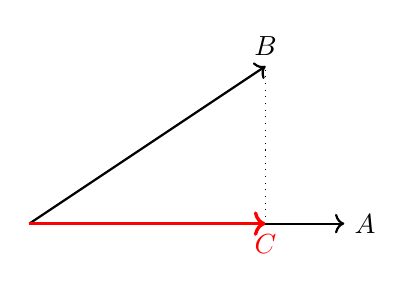
\begin{tikzpicture}
      % Draw vectors
      \draw[->, thick] (0,0) -- (3,2) node[above] { $B $ };%
      \draw[->, thick] (0,0) -- (4,0) node[right] { $A$ };%
      \draw[->, very thick, red] (0,0) -- (3,0) node[below] { $C$ };%
      \draw[dotted] (3,0) -- (3,2) ;%
      % % Label angle
      % \draw (1.2,0) arc[start angle=0, end angle=33.69, radius=1.2cm];%
      % \node at (1.5,0.4) {};%
    \end{tikzpicture}
  \end{center}
  In other words, $C$ is the shadow of $B$ on $A$, if we shine a light
  directly above $B$. This is an orthogonal projection because the dotted line
  is orthogonal to $A$.

  Let's work out an example. Suppose
  \begin{equation*}
    \vec{A} =
    \begin{bmatrix}
      1\\1\\2
    \end{bmatrix}
    \quad \text{and} \quad
    \vec{B}=
    \begin{bmatrix}
      -2\\3\\1
    \end{bmatrix}.
  \end{equation*}
  Then by \cref{eq:vector-projection-formula}, the vector projection is
  \begin{equation*}
    C =
    \begin{bmatrix}
      1/2\\1/2\\1
    \end{bmatrix}.
  \end{equation*}
  \textbf{Can we find a matrix $P$ that effectuates this transformation? That
    is, such that $PB=C$?}

  In general, the matrix for an orthogonal projection can be written as
  \begin{equation}\label{eq:orthogonal-projection-matrix}
    P = U(U^{\top}U)^{-1}U^{\top},
  \end{equation}
  where $U$ is any matrix whose columns form a basis of the subspace onto
  which we are projecting. In the case of the vector projection of $B$ onto
  $A$, we are projecting onto the line spanned by the vecctor $A$. Hence, we
  can take
  \begin{equation*}
    U =
    \begin{bmatrix}
      1\\1\\2
    \end{bmatrix}.
  \end{equation*}
  Now let's compute $P$. First observe that
  \begin{equation*}
    U^{\top}U =
    \begin{bmatrix}
      1&1&2
    \end{bmatrix}
    \begin{bmatrix}
      1\\1\\2
    \end{bmatrix}
    =
    1+1+4=6,
  \end{equation*}
  so
  \begin{equation*}
    (U^{\top}U)^{-1} = \frac{1}{6}.
  \end{equation*}
  Plugging this into \cref{eq:orthogonal-projection-matrix}, we get
  \begin{equation*}
    P =
    \frac{1}{6}
    \begin{bmatrix}
      1\\1\\2
    \end{bmatrix}
    \begin{bmatrix}
      1&1&2
    \end{bmatrix}
    =
    \frac{1}{6}
    \begin{bmatrix}
      1&1&2\\
      1&1&2\\
      2&2&4
    \end{bmatrix}.
  \end{equation*}
  Now we can check that $PB=C$:
  \begin{equation*}
    PB = \frac{1}{6}
    \begin{bmatrix}
      1&1&2\\
      1&1&2\\
      2&2&4
    \end{bmatrix}
    \begin{bmatrix}
      -2\\3\\1
    \end{bmatrix}
    =
    \frac{1}{6}
    \begin{bmatrix}
      -2+3+2\\
      -2+3+2\\
      -4+6+4
    \end{bmatrix}
    = \frac{1}{6}
    \begin{bmatrix}
      3\\
      3\\
      6
    \end{bmatrix}
    =
    \begin{bmatrix}
      1/2\\1/2\\1
    \end{bmatrix}
    =C.
  \end{equation*}
\end{example}

\begin{example}[Reflection]
  Reflection across the $\theta$-line (i.e. the line passing through the
  origin with angle $\theta$) is given by the following matrix:
  \begin{equation*}
    H =
    \begin{bmatrix}
      2c^{2}-1&2cs\\
      2cs&2s^{2}-1
    \end{bmatrix}
  \end{equation*}
  where $c=\cos(\theta)$ and $s=\sin(\theta)$.

  Observe
  \begin{equation*}
    H^{2}=H
  \end{equation*}

  \begin{equation*}
    H = 2P-I
  \end{equation*}

  For example, $\theta=90^{\circ}$ gives
  \begin{equation*}
    H =
    \begin{bmatrix}
      0&1\\
      1&0
    \end{bmatrix}
  \end{equation*}
\end{example}



\newpage
\section{2025-10-29 | Week 10 | Lecture 28}
\begin{center}
  \begin{tcolorbox}[width=0.9\textwidth, colback=white, colframe=black]
    \textit{\textbf{The nexus question of this lecture:} What are eigenvalues
      and eigenvectors and how do we find them?}
  \end{tcolorbox}
\end{center}

One way to understand what a linear linear transformation does is to undertand
which parts of space are invariant --- that is, which parts of space don't
change. 

\subsection{Eigenvalues}


\begin{definition}[Eigenvalue,eigenvector]
  \label{def:eigenvalue-eigenvector}
  If $A$ is an $n\times n$ matrix, an \demph{eigenvector} of $A$ is a nonzero
  column vector $v\in \R^{n}$ such that
  \begin{equation*}
    Av=\lambda v
  \end{equation*}
  for some scalar $\lambda\in \C$. The scalar $\lambda$ is called an \demph{eigenvalue}.
\end{definition}

\begin{example}
  Let
  \begin{equation*}
    A=\frac{1}{2}
    \begin{bmatrix}
      3&1\\1&3
    \end{bmatrix}
  \end{equation*}
  In \cref{ex:composing-transformations}, we say that this transformation
  corresponds to a dilation by a factor of $2$ in the direction of
  $45^{\circ}.$

  By geometric considerations, we can see that the line $y=x$ is invariant
  under this transformation (vectors along this line get scaled by 2 but don't
  jump off the line). Also we see that the line $y=-x$ is invariant (vectors
  along this line don't change at all).

  The vector $v =
  \begin{bmatrix}
    1\\1
  \end{bmatrix}
  $
  lies on the line $y=x$. We see that
  \begin{equation*}
    Av = 2v
  \end{equation*}
  so that $v=
  \begin{bmatrix}
    1\\1
  \end{bmatrix}
  $ is an eigenvector with eigenvalue $2$.

  Similarly, the following vector lies on the line $y=-x$:
  \begin{equation*}
    v=
    \begin{bmatrix}
      1\\-1
    \end{bmatrix}
  \end{equation*}
  It satisfies $Av=1v$. Hence it is an eigenvector with eigenvalue $1$.
\end{example}

\begin{example}
  Let
  \begin{equation*}
    A=
    \begin{bmatrix}
      1&-3\\
      -2&2
    \end{bmatrix}
  \end{equation*}
  has eigenvewctor
  \begin{equation*}
    v=
    \begin{bmatrix}
      -1\\1
    \end{bmatrix}
  \end{equation*}
  with eigenvalue $4$.
\end{example}


\subsection{How do we find eigenvalues?}

\textbf{Idea:} look to the system
$AX =\lambda X$.
This is equivalent to 
\begin{equation*}
  (\lambda I-A)X=0.
\end{equation*}
Since $X\neq 0$ (since by definition eigenvectors must be nonzero), we
conclude that the matrix $\lambda I - A$ is singular, and hence by the key
theorem, $\det(\lambda I -A)=0$. 

\begin{theorem}
  Let $A$ be an $n\times n$ matrix. Then $\lambda\in \R$ is an eigenvalue of
  $A$ if and only if $\det(\lambda I-A)=0$.
\end{theorem}


\begin{definition}
  The \demph{characteristic equation of $A$ } is
  \begin{equation*}
    \det(\lambda I-A)=0.
  \end{equation*}
\end{definition}
When $A$ is an $n\times n$ matrix, the left hand side of the characteristic
equation is a polynomial in the variable $\lambda$ of degree $n$, and is
called the \demph{characteristic polynomial} of $A$.


\begin{example}
  Let
  \begin{equation*}
    A =
    \begin{bmatrix}
      1&-3\\-2&2
    \end{bmatrix}.
  \end{equation*}
  Then the characteristic polynomial of $A$ is
  \begin{align*}
    \det(\lambda I-A) 
    &= \det
      \begin{bmatrix}
        \lambda-1& 3\\
        2& \lambda-2
      \end{bmatrix} \\
    &=(\lambda-1)(\lambda-2)-6\\
    &=\lambda^{2}-3\lambda-4\\
    &(\lambda-4)(\lambda+1)
  \end{align*}
  This is equal to zero if and only if $\lambda=4$ or $\lambda=-1$. Therefore
  the eigenvalues of $A$ are $\lambda=4$ and $\lambda=-1.$ 
\end{example}


\subsection{How do we find eigenvectors?}

\textbf{Idea:} First find the eigenvalues $\lambda$. Then for each eigenvalue
$\lambda$, the eigenvectors are the nontrivial solutions of the homogeneous
ssytem
\begin{equation*}
  (\lambda I-A)X =0.
\end{equation*}
(This is a linear system which we can solve using row reduction.)

In other words, the eigenvectors are the nonzero vectors in the linear
subspace
\begin{equation*}
  NS(\lambda I-A).
\end{equation*}
So we just need to compute a basis of this nullspace, which is called the
\demph{eigenspace}. When we ask to find the eigenvalues, it is always enough
to just compute the basis of the eigenspace.




\begin{example}
  Find the eigenvectors of the matrix
  \begin{equation*}
    A=
    \begin{bmatrix}
      1&-3\\
      -2&2
    \end{bmatrix}
  \end{equation*}
  The equations we need to solve are
  \begin{itemize}
    \item \textbf{When $\lambda=4$:} $4I-A=0$ or
    \begin{equation*}
      \begin{bmatrix}
        3&3\\
        2&2
      \end{bmatrix}
      \begin{bmatrix}
        x\\y
      \end{bmatrix}
      =
      \begin{bmatrix}
        0\\0
      \end{bmatrix}
    \end{equation*}
    Reducing find the nullspace is
    \begin{equation*}
      NS(4I-A) = \left\{y 
        \begin{bmatrix}
          -1\\1
        \end{bmatrix}, \, y\in \R
      \right\} 
    \end{equation*}
    Technically, all vectors in $NS(4I-A)$ are eigenvectors for $\lambda=4$.
    To give a concrete example, we have eigenvector $v=
    \begin{bmatrix}
      -1\\1
    \end{bmatrix}$.
    
    % \item \textbf{When $\lambda=-1$:} $-I-A=0$
    % Here we get a NS generated by a single basis element $
    % \begin{bmatrix}
    %   3\\2
    % \end{bmatrix}
    % $
  \end{itemize}
\end{example}
\newpage
\section{2025-11-03 | Week 11 | Lecture 29}

\begin{example}
  \Fl{Question:} Find the eigenvalues and eigenvectors of
  \begin{equation*}
    A=
    \begin{bmatrix}
      1&-1\\1&1
    \end{bmatrix}
  \end{equation*}
  This is a rotation by $45^{\circ}$ composed with a scaling by $\sqrt{2}$.
  That is, $A=\sqrt{2}R_{45^{\circ}}$.
  
  \Fl{Solution:} The characteristic equation is
  \begin{equation*}
    \det
    \begin{bmatrix}
      \lambda-1&1\\-1&\lambda-1
    \end{bmatrix}
    = (\lambda-1)^{2}+1 = \lambda^{2}-2\lambda +2=0
  \end{equation*}
  This has solutions
  \begin{equation*}
    \lambda=1\pm i
  \end{equation*}
  \begin{itemize}
    \item For $\lambda=1+i$, solve  $((1+i)I-A)X=0$. This has solution
    \begin{equation*}
      \begin{bmatrix}
        x\\y
      \end{bmatrix}
      =
      \begin{bmatrix}
        iy\\y
      \end{bmatrix}
      =
      \begin{bmatrix}
        i\\1
      \end{bmatrix}y
    \end{equation*}
    where $y$ is any complex number. A basis for this is
    \begin{equation*}
      \begin{bmatrix}
        i\\1
      \end{bmatrix}.
    \end{equation*}
    This is the eigenvector
    \item For $\lambda=1-i$, similar calculation gives an eigenvector
    \begin{equation*}
      \begin{bmatrix}
        -i\\1
      \end{bmatrix}
    \end{equation*}
  \end{itemize}
  
\end{example}



\begin{example}
  Find the eigenvals and eigenvectors of
  \begin{equation*}
    \begin{bmatrix}
      2&-1&3\\
      0&-1&0\\
      0&0&-1
    \end{bmatrix}
  \end{equation*}
  First we compute the characteristic polynomial:
  \begin{equation*}
    \det(\lambda I-A) = ... = (\lambda-2)(\lambda+1)^{2}
  \end{equation*}
  This equals zero iff $\lambda=2$ or $\lambda=-1$. These are the
  eigvenvalues.

  To find eigenvectors, we need to find a basis nfor the nullspaces $NS(2I-A)$
  and $NS(-I-A)$.
\end{example}


\newpage
\section{Another example}

\begin{example}[Differentiation of polynomials]
  Consider $P_{3}= \left\{p\in \R[x]: \deg (p) \leq 3\right\} $. 
  Given an element $p\in P_{3}$, we have $p(x)=
  c_{0}+c_{1}x+c_{2}x^{2}+c_{3}x^{3}$. A basis for $P_{3}$ is
  \begin{equation*}
    \beta= \left\{\beta_{1}= 1,\quad \beta_{2}=x, \quad \beta_{3}=x^{2}, \quad \beta_{4}=x^{3}\right\} 
  \end{equation*}

  Let $D = \frac{d}{dt}$. We've already seen that $D: P_{3}\to P_{3}$ is a
  linear transformation (see \cref{ex:derivative-is-a-linear-transformation}).

  \Fl{Question:} What is $[T]_{\beta}^{\beta}$, the matrix of $T$ with
  respect to the basis $\beta$?

  \fl{Idea:} First, we consider how  $D=\frac{d}{dt}$ acts on the vectors
  $\beta_{1},\beta_{2},\beta_{3}$, and write the output in terms of the
  vectors $\beta_{1},\beta_{2},\beta_{3}$. 

  \fl{Solution:} Observe that
  \begin{equation*}
    D\beta_{1} = 0, \quad D\beta_{2}=\beta_{1}, \quad D\beta_{3}=2\beta_{2}, \quad D\beta_{4}=3\beta_{3} 
  \end{equation*}

  The matrix for $\frac{d}{dx}$ with respect to the basis $\beta$ is
  \begin{equation*}
    [D]_{\beta}^{\beta}
    =\begin{bmatrix}
      0&1&0&0\\
      0&0&2&0\\
      0&0&0&3\\
      0&0&0&0
    \end{bmatrix}
  \end{equation*}
  For example, if $p(x)=3+5x-7x^{2}+2x^{3}$, we can write $p$ as
  \begin{equation*}
    p =
    \begin{bmatrix}
      3\\5\\-7\\2
    \end{bmatrix}_{\beta}
  \end{equation*}
  In which case
  \begin{equation*}
    [D]_{\beta}^{\beta}p =\begin{bmatrix}
      0&1&0&0\\
      0&0&2&0\\
      0&0&0&3\\
      0&0&0&0
    \end{bmatrix}
    \begin{bmatrix}
      3\\5\\-7\\2
    \end{bmatrix}_{\beta}
    =
    \begin{bmatrix}
      5\\-14\\6\\0
    \end{bmatrix}_{\beta}
  \end{equation*}
  The ``coordinate vector'' notation on the right hand side means the
  following:
  \begin{equation*}
    \begin{bmatrix}
      5\\-14\\6\\0
    \end{bmatrix}_{\beta}
    =5\beta_{1}-14\beta_{2}+6\beta_{3}+0\beta_{4} = 5-14x+6x^{2}.
  \end{equation*}
  It worked! This is the derivative of $p(x) = 3+5x-7x^{2}+2x^{3}$.


  \fl{What about integration?}
\end{example}


\newpage
\end{document}



